 \documentclass[a4paper,11pt]{amsart}

%     If you need symbols beyond the basic set, uncomment this command.
%\usepackage{amssymb}

%     If your article includes graphics, uncomment this command.
%\usepackage{graphicx}

%     If the article includes commutative diagrams, ...
%\usepackage[cmtip,all]{xy}


%     Update the information and uncomment if AMS is not the copyright
%     holder.
%\copyrightinfo{2009}{American Mathematical Society}

\usepackage{amssymb}
\usepackage{amscd}
\usepackage{amsthm}
%\usepackage[dvips]{graphicx}
\usepackage{amsmath}
\usepackage[all]{xy}
\usepackage{extarrows}
\usepackage{rotating}
\usepackage{tikz-cd}
\usepackage{quiver}
\usepackage{leftidx}
\usepackage{bm}
\usepackage{dynkin-diagrams}
\usepackage{mathrsfs}
%\usepackage{hyperref}
\usepackage{rotating}
\usepackage{upgreek}
\usepackage{thmtools}

%%%%%%

\declaretheorem{theorem} 
\declaretheoremstyle[%
spaceabove=-6pt,%
spacebelow=6pt,%
%headfont=\normalfont\itshape,%
postheadspace=0.5em,%
qed=\qedsymbol,%
headpunct={}
]{mystyle} 
\declaretheorem[name={Proof},style=mystyle,unnumbered,
]{Proof}

%\usepackage[pagebackref]{hyperref}

%\usepackage[backref=page]{hyperref}

%\usepackage[pagebackref=true]{hyperref}
\usepackage{hyperref}

%\renewcommand*{\backref}[1]{}
%\renewcommand*{\backrefalt}[4]{[{\tiny%
%		\ifcase #1 Not cited.%
%		\or Cited on page~#2.%
%		\else Cited on pages #2.%
%		\fi%
%	}]}


\tikzset{
	symbol/.style={
		draw=none,
		every to/.append style={
			edge node={node [sloped, allow upside down, auto=false]{$#1$}}}
	}
}

%\usepackage[breaklinks,colorlinks,linkcolor=black,citecolor=black,urlcolor=black]{hyperref}

\DeclareUnicodeCharacter{2212}{-}
\DeclareUnicodeCharacter{0008}{~}
\DeclareUnicodeCharacter{2011}{~}


\def\mathbi#1{\textbf{\em #1}}

\renewenvironment{proof}{{ \textbf{Proof}.}}{\qed}


\newtheorem{Thm}{Theorem}[section]
\newtheorem{Lem}[Thm]{Lemma}
\newtheorem{lemma}[Thm]{Lemma}
\newtheorem{Def}[Thm]{Definition}
\newtheorem{Cor}[Thm]{Corollary}
\newtheorem{Prop}[Thm]{Proposition}
\newtheorem{Ex1}[Thm]{Example}
\newtheorem{Rem1}[Thm]{Remark}
\newtheorem{Conj}[Thm]{Conjecture}
\newtheorem{assumption}{Assumption}
\newcommand{\Ima}{\mathrm{Im}}
\newcommand{\coker}{\mathrm{coker}}
\newcommand{\cone}{\mathrm{Cone}}
\newcommand{\Hom}{\mathrm{Hom}}
\newcommand{\thick}{\mathrm{thick}}
\newcommand{\add}{\mathrm{add}}
\newcommand{\per}{\mathrm{per}}
\newcommand{\Ext}{\mathrm{Ext}}
\newcommand{\End}{\mathrm{End}}
\newcommand{\obj}{\mathrm{obj}}
\newcommand*{\isoarrow}[1]{\arrow[#1,"\rotatebox{90}{\(\sim\)}"]}
\newcommand{\bijar}[1][]{%
	\ar[#1]
	\ar@<0.7ex>@{}[#1]|-*[@]{\sim}} 

\newcommand{\lG}{\mathbi{L}G^{*}}
\newcommand{\lQ}{\mathbi{L}Q^{*}}
\newcommand{\pvd}{\mathrm{pvd}}
\newcommand*{\corner}{{}{\LARGE{$\ulcorner$}}}
\newcommand{\hten}{\hat{\otimes}}
\newcommand{\cten}{\widehat{\otimes}}
\newcommand{\tor}{\mathrm{Tor}}
\newcommand{\Bd}{\mathrm{Bd}}
\newcommand{\PcAlgc}{\mathrm{PcAlgc}(R)}
\newcommand{\PcAlg}{\mathrm{PcAlg}(R)}
\newcommand{\ind}{\mathrm{ind}}
\newcommand{\copr}{\mathrm{copr}}


\newenvironment{Rem}{\begin{Rem1}\rm}{\end{Rem1}}
\newenvironment{Ex}{\begin{Ex1}\rm}{\end{Ex1}}

\newtheorem{condition}{Conditions}[section]

\setlength{\textwidth}{17.3cm} 
\setlength{\textheight}{25cm}%25 18
\setlength{\topmargin}{-0.0cm} 
\setlength{\oddsidemargin}{-1cm}
\setlength{\evensidemargin}{-1cm}
\setlength{\abovedisplayskip}{3mm}
\setlength{\belowdisplayskip}{3mm}
\setlength{\abovedisplayshortskip}{2mm}
\setlength{\belowdisplayshortskip}{2mm} \normalbaselines
\raggedbottom



% BK's commands


\newcommand{\Si}{\Sigma}
\newcommand{\La}{\Lambda}
\newcommand{\si}{\sigma}
\newcommand{\we}{\wedge}
\newcommand{\ten}{\otimes}
\newcommand{\lten}{\overset{\mathbf{L}}{\ten}}
\newcommand{\lcten}{\widehat{\ten}^{\boldmath{L}}}

\newcommand{\fib}{\mathrm{fib}}
\newcommand{\cof}{\mathrm{cof}}
\newcommand{\RHom}{\mathrm{\mathbf{R}Hom}}
\newcommand{\ra}{\rightarrow}
\newcommand{\la}{\leftarrow}
\newcommand{\iso}{\xrightarrow{_\sim}}
\newcommand{\liso}{\xleftarrow{_{\sim}}}
\newcommand{\id}{\mathbf{1}}
\renewcommand{\qedsymbol}{$\surd$}
\newcommand{\bmgamma}{\bm\Gamma}
\newcommand{\pr}{\mathrm{pr}}
\newcommand{\Gammabf}{\bm\Gamma}
\newcommand{\relGammabf}{\bm\Gamma}%%%%rel
\newcommand{\overGamma}{\overline{\bmgamma}}
\newcommand{\Gr}{\mathrm{Gr}}
\newcommand{\Mod}{\mathrm{Mod}}
\renewcommand{\mod}{\mathrm{mod}}
\newcommand{\coind}{\mathrm{coind}}
\newcommand{\downmapsto}{\rotatebox[origin=c]{-90}{$\scriptstyle\mapsto$}\mkern2mu}
\newcommand{\overc}{\overline{\cc}}


%
% BK's calligraphic letters
%
\newcommand{\ca}{{\mathcal A}}
\newcommand{\cb}{{\mathcal B}}
\newcommand{\cc}{{\mathcal C}}
\newcommand{\cd}{{\mathcal D}}
\newcommand{\ce}{{\mathcal E}}
\newcommand{\cf}{{\mathcal F}}
\newcommand{\cg}{{\mathcal G}}
\newcommand{\ch}{{\mathcal H}}
\newcommand{\ci}{{\mathcal I}}
\newcommand{\ck}{{\mathcal K}}
\newcommand{\cl}{{\mathcal L}}
\newcommand{\cm}{{\mathcal M}}
\newcommand{\cn}{{\mathcal N}}
\newcommand{\co}{{\mathcal O}}
\newcommand{\cp}{{\mathcal P}}
\newcommand{\cR}{{\mathcal R}}
\newcommand{\cq}{{\mathcal Q}}
\newcommand{\cs}{{\mathcal S}}
\newcommand{\ct}{{\mathcal T}}
\newcommand{\cu}{{\mathcal U}}
\newcommand{\cv}{{\mathcal V}}
\newcommand{\cw}{{\mathcal W}}
\newcommand{\cx}{{\mathcal X}}
\newcommand{\cy}{{\mathcal Y}}
\newcommand{\cz}{{\mathcal Z}}

\newcommand{\T}{\mathbb{T}}
\renewcommand{\P}{\mathbb{P}}
\newcommand{\Q}{\mathbb{Q}}
\newcommand{\Z}{\mathbb{Z}}
\newcommand{\C}{\mathbb{C}}
\newcommand{\R}{\mathbb{R}}

\renewcommand{\phi}{\varphi}

\newcommand{\ko}{\;\;, }
\newcommand{\ie}{i.e.~}

\newcommand{\ol}[1]{\overline{#1}}
\newcommand{\ul}[1]{\underline{#1}}
\renewcommand{\hat}[1]{\widehat{#1}}
\renewcommand{\tilde}[1]{\widetilde{#1}}




\begin{document}
	
	% \title[short text for running head]{full title}
	\title[]{Relative cluster categories and Higgs categories\\ with infinite-dimensional morphism spaces}
	
	%    Only \author and \address are required; other information is
	%    optional.  Remove any unused author tags.
	
	%    author one information
	% \author[short version for running head]{name for top of paper}
	
	
	\author{Bernhard Keller and 
		Yilin WU}
	\address{
		Universit\'e Paris Cit\'e\\
		UFR de Math\'ematiques\\
		Institut de Math\'ematiques de Jussieu--Paris Rive Gauche, IMJ-PRG \\
		B\^{a}timent Sophie Germain\\
		75205 Paris Cedex 13\\
		France
	}
	\email{bernhard.keller@imj-prg.fr}
	\urladdr{https://webusers.imj-prg.fr/~bernhard.keller/}
	
	
	
	
%	\address{
%		Department of Mathematics, East China Normal University,
%		Shanghai 200241, China\\
%		and
%		Universit\'e Paris Cit\'e\\
%		UFR de Math\'ematiques\\
%		Institut de Math\'ematiques de Jussieu--Paris Rive Gauche, IMJ-PRG \\
%		B\^{a}timent Sophie Germain\\
%		75205 Paris Cedex 13\\
%		France
%	}
%	\email{wuyilinecnuwudi@gmail.com\\
%		yilin.wu@imj-prg.fr}
\address{
	School of Mathematical Sciences\\
	University of Science and Technology of China\\
    Hefei 230026, Anhui\\
	P. R. China}
\email{wuyilinecnuwudi@gmail.com}
\urladdr{https://webusers.imj-prg.fr/~yilin.wu/}
	%    \subjclass is required.
	%\subjclass[2010]{18G35, 13F60, 16E35}
	
	%\date{\today}
	
	\dedicatory{}
	
	\keywords{Ice quiver with potential, relative Ginzburg algebra, Higgs category, cluster character, quasi-cluster homomorphism}
	
	%    Abstract is required.
\begin{abstract}
Cluster algebras {\em with coefficients} are important since they appear in nature as coordinate algebras of varieties like Grassmannians, double Bruhat cells, unipotent cells, $ \cdots $. The work of 
Geiss--Leclerc--Schröer often yields Frobenius exact categories which allow to categorify such cluster algebras. In previous work, the second-named author has constructed Higgs categories and relative cluster categories in the relative Jacobi-finite setting (arXiv:2109.03707). Higgs categories generalize the Frobenius categories used by Geiss--Leclerc--Schr\"oer.
		 
In this article, we construct the Higgs category and the relative cluster category in the 
relative Jacobi-infinite setting under suitable hypotheses. This covers for example the case
of Jensen--King--Su's Grassmannian cluster category.
As in the relative Jacobi-finite case, 
the Higgs category is no longer exact  but still extriangulated in the sense of Nakaoka-Palu.
We also construct a cluster character refining Plamondon's. 

In the appendix, Chris Fraser and the first-named author categorify quasi-cluster morphisms using 
Frobenius categories. A recent application of this result is due to Matthew Pressland, who uses it to 
prove a conjecture by Muller--Speyer.
\end{abstract}
	
	\dedicatory{{\rm With an appendix by Chris Fraser and Bernhard Keller} \\[0.5cm]
	Dedicated to Professor Henning Krause on the occasion of his 60th birthday}
	
	\maketitle
	%    Text of article.
	
	\setcounter{tocdepth}{1}
	
	\tableofcontents
	
	\section{Introduction}	
Cluster categories were introduced in 2006 by Buan-Marsh-Reineke-Reiten-Todorov
\cite{buanClusterStructures2Calabi2009} in order to categorify acyclic 
cluster algebras  \cite{fominClusterAlgebrasFoundations2002a, fominsergeyTotalPositivityCluster, FominWilliamsZelevinsky16}
without  coefficients. Caldero and Chapoton used the geometry of 
quiver  Grassmannians to define the cluster character~\cite{Caldero-Chapot2006}, i.e. a decategorification map 
which yields a bijection from the set of isomorphism classes of indecomposable objects of the cluster category of a Dynkin quiver to the set of cluster variables in the associated cluster algebra. More generally, for (antisymmetric) cluster algebras
associated with acyclic quivers, Caldero-Keller \cite{Caldero-Keller2008} showed that the
Caldero-Chapoton map induces a bijection between the set of isomorphism classes of indecomposable rigid objects 
and the set of cluster variables.
	
In order generalize the representation-theoretic approach to cluster algebras from acyclic quivers
to quivers with oriented cycles, Derksen--Weyman--Zelevinsky 
\cite{DerksenWeymanZelevinsky08, DerksenWeymanZelevinsky10} extended the
mutation operation from quivers to quivers with potential and their representations. 
In the case where the quiver with potential
is Jacobi-finite, Amiot~\cite{amiotClusterCategoriesAlgebras2009} generalized
the construction of the cluster category~\cite{amiotClusterCategoriesAlgebras2009}. 
The cluster character constructed by Palu in~\cite{paluClusterCharacters2Calabi2008} induces a
bijection \cite{CerulliKellerLabardiniPlamondon2013} from the isoclasses of the 
reachable rigid indecomposables of the 
(generalized) cluster category to the cluster variables of the associated cluster algebra.
Plamondon~\cite{plamondonCategoriesAmasseesAux2011} generalized Amiot's and
Palu's constructions to arbitrary quivers with potential.
	
Cluster algebras with coefficients are of great importance in geometric examples. They appear in nature as coordinate algebras of varieties like Grassmannians, double Bruhat cells, unipotent cells, \ldots\ cf.~for example \cite{Berenstein-Fomin-Zelevinsky2005,GLS2010,scottGrassmanniansClusterAlgebras2006}. The work of Geiss--Leclerc--Schr\"oer provides Frobenius exact categories which allow to categorify such cluster algebras~\cite{GLS2006,GLS2010} in
many cases. In their approach, the Frobenius exact category is a full subcategory of the
category of modules over a certain preprojective algebra. Geiss--Leclerc--Schr\"oer's setting was
axiomatized by Fu--Keller \cite{Fu-Keller2010} using stably $2$-Calabi--Yau Frobenius categories.
They also observed that not all cluster algebras with coefficients admit such a categorification 
(for example, acyclic cluster algebras with principal coefficients do not, cf.~Remark~5.7 of  \cite{Fu-Keller2010}).

In order to extend Geiss--Leclerc--Schr\"oer's approach to larger classes of cluster algebras with coefficients,
the second-named author introduced relative cluster categories and Higgs categories in 
\cite{wuRelativeClusterCategories2021}. However, the setting he considered was restricted
to the case of ice quivers with potential $(Q,F,W)$ whose associated relative Jacobi algebra is
finite-dimensional. In this article, our aim is to construct the associated Higgs category $ \ch(Q,F,W) $
and the relative cluster category $ \cc(Q,F,W) $ under a much weaker assumption~(cf.~Assumption~\ref{assumption}). 
We also construct a canonical cluster character in this setting. Higgs categories generalize the 
Frobenius categories used by Geiss-Leclerc-Schröer. Our cluster character generalizes Plamondon's \cite{plamondonCategoriesAmasseesAux2011} to the relative context. 

Let us state our main results more precisely:	
Let  $(Q,F,W)$ be an ice quiver with potential and $ \relGammabf=\Gammabf(Q,F,W) $ the associated relative Ginzburg algebra (cf.~section~\ref{ss:Ginzburg algebras}).
Let $ e=\sum_{i\in F}e_{i} $ be the idempotent associated with the set of frozen vertices. 
Let $ J(Q,F,W)=H^0(\relGammabf)$ be the corresponding relative Jacobian algebra.
We denote by $ \cp=\add(e\relGammabf) $ the closure under finite direct sums and summands
of $e\relGammabf$ in the perfect derived category $ \per\relGammabf $. The {\em relative cluster
category $\cc(Q,F,W)$} is defined as the idempotent completion of the quotient of $\per\Gammabf$ by the thick subcategory
generated by all simple $H^0(\Gammabf)$-modules associated with non frozen vertices of $Q$.
The {\em Higgs category $\ch(Q,F,W)$} is a certain extension closed full subcategory of $\cc(Q,F,W)$
(cf.~Definition~\ref{Def: Higgs cat}).
Let $ (\overline{Q},\overline{W}) $ be the quiver with potential obtained from $ (Q,F,W) $ by deleting the frozen part $ F $ and $ \mathbf{\Gamma}(\overline{Q},\overline{W}) $ the Ginzburg algebra of $ (\overline{Q},\overline{W}) $. Then we have a dg quotient morphism 
\[
p\colon\relGammabf(Q,F,W)\ra\mathbf{\Gamma}(\overline{Q},\overline{W}).
\]
It induces a triangulated quotient functor $ p^{*}\colon\cc(Q,F,W)\ra\cc(\overline{Q},\overline{W}) $, where $ \cc(\overline{Q},\overline{W}) $ (or $ \overline{\cc} $) is the associated generalized cluster category.
Let  $ \cd(Q,F,W)\subseteq\cc(Q,F,W) $ be the full subcategory of $ \cc(Q,F,W) $ whose objects are the
$ M $ in $ \cc(Q,F,W) $ whose image $ p^{*}(M) $ lies in Plamondon's category $ \cd(\overline{Q},\overline{W}) $ 
(see Subsection~\ref{Subsection: Plamondon's category}). In the following theorem, we abbreviate
$\Gammabf=\Gammabf(Q,F,W)$ and $\ch=\ch(Q,F,W)$.
	
	\begin{Thm}(Theorem~\ref{Thm: main results})
		Let $ (Q,F,W) $ be an ice quiver with potential such that $ \cp=\add(e\relGammabf) $ is functorially finite in $ \add(\relGammabf) $.
		\begin{itemize}
			\item[1)] We have an equivalence of $ k $-categories
			$$ \ch(Q,F,W)/[\cp]\iso\cd(\overline{Q},\overline{W}) .$$
			\item[2)] If $ (\overline{Q},\overline{W}) $ is Jacobi-finite, then $ \ch(Q,F,W) $ is a Frobenius extriangulated category with projective-injective objects $ \cp=\add(e\bmgamma) $ and the equivalence in $ (1) $ preserves the extriangulated structure. Moreover, we have equalities $$ \cd(\overline{Q},\overline{W})=\cc(\overline{Q},\overline{W}) $$ and
			$$ \cd(Q,F,W)=\cc(Q,F,W). $$
			\item[3)] If moreover $ \bmgamma $ is concentrated in degree 0, then the \emph{boundary algebra} $ B\!=\!\! eH^{0}(\relGammabf)e $ is $ \mathrm{fp}_{\infty} $-Gorenstein of injective dimension at most $e$ with respect to $ \relGammabf $ and the Higgs category $ \ch $ is equivalent to the category $ \mathrm{gpr}_{\infty}^{\leqslant3}B $ (cf.~section~\ref{ss:IKW-theorem}). Moreover, $ \bmgamma $ is a canonical cluster-tilting object of $ \ch $ with endomorphism algebra $ \End_{\ch}(\bmgamma)=H^{0}(\relGammabf)=J(Q,F,W) $.
			\item[4)] Let $ \cm=\add(\bmgamma)\subseteq\ch $. Under the assumptions of $ 3) $, the exact sequence of triangulated categories
			$$ 0\ra\pvd_{e}(\bmgamma)\ra\per\bmgamma\ra\cc(Q,F,W)\ra0 $$
			is equivalent to
			$$ 0\ra\ck^{b}_{\ch-ac}(\cm)\ra\ck^{b}(\cm)\ra\cd^{b}(\ch)\ra0. $$
			In particular, the relative cluster category $ \cc(Q,F,W) $ is equivalent to the bounded derived category $ \cd^{b}(\ch) $ of $ \ch $.
		\end{itemize}	
		
	\end{Thm}
%	Here $ \cd(\overline{Q},\overline{W}) $ is Plamondon's category (see Definition~\ref{Def:Plamondon's cat}) and $ \cc(\overline{Q},\overline{W}) $ is the generalized cluster category. 
    
In section~\ref{s:cluster characters},  we generalize Fu-Keller's cluster character to a cluster character
\[
CC=X_{?}\colon\obj(\ch)\ra\mathbb{Q}[x_{r+1},\ldots,x_{n}][x_{1}^{\pm1},x_{2}^{\pm1},\ldots,x_{r}^{\pm1}]
\]
defined for Hom-infinite Higgs categories $\ch$. Thus, the Higgs category yields an additive categorification for cluster algebras with {\em non-invertible} coefficients and the cluster character is a decategorification map.
Let us point out that Grabowski and Pressland will construct a cluster character for certain extriangulated categories 
in their upcoming paper \cite{Grabowsk-Pressland2023}.

Now we assume that $ (\overline{Q},\overline{W}) $ is Jacobi-finite. By definition, the Higgs category $ \ch(Q,F,W) $ is a full subcategory of $ \cc(Q,F,W) $. The following theorem shows that the map $CC$ defined on $\ch(Q,F,W)$
canonically extends to a map
\[
CC_{loc}\colon\cc(Q,F,W)\ra\mathbb{Q}[x_{1}^{\pm1},\ldots,x_{r}^{\pm1},x_{r+1}^{\pm1},\ldots,x_{n}^{\pm1}]
\]
defined on the {\em whole} relative cluster category.
Thus, we can consider the triangulated category $ \cc(Q,F,W) $ as an additive categorification of a cluster algebra
with {\em invertible} coefficients and the map $ CC_{loc} $ as a decategorification map.

\begin{Thm}(Theorem~\ref{Thm: commutative diagram})
	Let $ (Q,F,W) $ be an ice quiver with potential such that $ \cp=\add(e\relGammabf) $ is functorially finite in $ \add(\relGammabf) $. We assume moreover that $ (\overline{Q},\overline{W}) $ is Jacobi-finite.
	Consider the following diagram, where
	$\ol{CC}$ is the cluster character constructed by Plamondon in~\cite{plamondonCategoriesAmasseesAux2011},
	\[
	\begin{tikzcd}
		\ch\arrow[dd,"p^{*}"]\arrow[r,hook]&\cc(Q,F,W)
		%\thick_{\cc}\langle\cp\rangle*\Si^{\mathbb{Z}}\ch
		\arrow[r,dashed,"CC_{loc}"]&\mathbb{Q}[x_{1}^{\pm1},\ldots,x_{r}^{\pm1},x_{r+1}^{\pm1},\ldots,x_{n}^{\pm1}]\arrow[dd,"{x_{i}\mapsto1,}\,\,\forall i>r"] \\
		\\
		\underline{\ch}\arrow[r,"\sim"]&\cc(\overline{Q},\overline{W})\arrow[r,"\overline{CC}"]&\mathbb{Q}[x_{1}^{\pm1},\ldots,x_{r}^{\pm1}].
	\end{tikzcd}	
	\]
	There is a unique map $$ CC_{loc}\colon\cc(Q,F,W)
	%\thick_{\cc}\langle\cp\rangle*\Si^{\mathbb{Z}}\ch
	\to\mathbb{Q}[x_{1}^{\pm1},\ldots,x_{r}^{\pm1},x_{r+1}^{\pm1},\ldots,x_{n}^{\pm1}] $$
	such that the above diagram commutes and 
	\begin{itemize}
		\item[1)] for each triangle in $ \cc(Q,F,W) $
		$$ P\ra X\ra M\ra\Si P $$ with $ P\in\thick_{\cc}(\cp) $,
		%and $ M\in\Si^{\mathbb{Z}}\ch $
		we have 
		$$ CC_{loc}(X)=CC_{loc}(P)\cdot CC_{loc}(M)\, ;$$
		\item[2)] the restriction $ CC_{loc}|_{\ch} $ is the cluster character $ X_{?} $ defined 
		in~Section~\ref{s:cluster characters}.
		%	\item[3)] for each object $ X\in\ch $ 
		%	without non-zero direct summands in $ \cp $, we have
		%	$$ CC_{loc}(X)=x^{\mathrm{g_{fr}}(X)}\cdot\overline{CC}(p^{*}(X)); $$
		\item[3)] for each object $ P $ in $ \thick_{\cc}(\cp)$, we have $ CC_{loc}(P)=x^{[P]} $, where $ [P]\in K_{0}(\per\bmgamma)\simeq\mathbb{Z}^{n} $.
	\end{itemize}
\end{Thm}
%Here $ \mathrm{g_{fr}} $ is the following map
%$$ \ch\hookrightarrow\pr_{\cc}\relGammabf\cap\copr_{\cc}\relGammabf\simeq\pr_{\cd}\relGammabf\cap\copr_{\cd}\relGammabf
%$$  $$\hookrightarrow\per\bmgamma\ra K_{0}(\per\bmgamma)\cong\mathbb{Z}^{n}\xrightarrow{\text{frozen part}}\mathbb{Z}^{n-r} .$$

This article is organized as follows. In Section~\ref{Section: ice quiver} we first recall the definitions of ice quivers with potential and the mutation operations. Then we give the construction of (complete) relative Ginzburg algebras. In Section~\ref{Section: Relative cluster categories and Higgs Categories}, we use Plamondon's technique to 
define the Higgs category. The relationship between the Higgs category and Plamondon's category is explained in Section~\ref{Subsection: Plamondon's category}. 

Let $ (Q,F,W) $ be an ice quiver with potential and $ \mu_{v}(Q,F,W)=(Q',F',W') $ its mutation at a vertex $v$. If $ v $ is an unfrozen vertex, we show that mutation at $ v $ yields an equivalence between the relative cluster categories 
of $(Q,F,W)$ and $(Q',F',W')$ 
(see Proposition~\ref{Prop: mutation at unfrozen}). If $ v $ is a frozen source or frozen sink, 
the mutation at $ v $ yields an equivalence between $ \cd(Q,F,W) $ and $ \cd(Q',F',W') $ 
(see Proposition~\ref{Rem: mutation at frozen}).

Section~\ref{Section: Cluster characters} is devoted to the construction of the cluster character $ CC=X_{?} $
 (with respect to $ \relGammabf $) on $ \ch(Q,F,W) $. We use an argument similar to Plamondon's to show the multiplication formula, cf.~Section~\ref{Subsection: Multiplication formula}. Then we extend our cluster character 
 to a map 
 \[
 CC_{loc}\colon\cc(Q,F,W)\ra\mathbb{Q}[x_{1}^{\pm1},\ldots,x_{r}^{\pm1},x_{r+1}^{\pm1},\ldots,x_{n}^{\pm1}].
 \]
 In Section~\ref{Section: Applications to quasi-cluster homomorphisms}, we show that the 
decategorification of the equivalence associated with the mutation at a frozen source (or sink) is a quasi-cluster isomorphism. In the final section~\ref{s:Postnikov diagrams}, we explain how the class of ice quivers with potential which come from Postnikov diagrams fits into the theory developed in this article. 

In appendix~\ref{appendix}, Chris Fraser and the first-named author use 
Frobenius categorifications (which can often be
constructed using the main results of this paper) to construct quasi-cluster isomorphisms. 
In \cite{presslandMuller-Speyer conjecture}, Matthew Pressland has recently applied these results to prove a 
conjecture by Muller--Speyer \cite[Rem.~4.7]{muller-speyer2017} linking the two canonical cluster structures 
on a positroid variety by a quasi-cluster isomorphism.

%\textcolor{red}{We would like to remark that Pressland~\cite{presslandMuller-Speyer conjecture} recently confirms a phenomenon observed by Muller--Speyer~\cite{muller-speyer2017}, which states that the source and target labelled cluster structures on a positroid variety quasi-coincide when the positroid is connected, by means of categorification.} 
	
\section*{Acknowledgments}
The second-named author thanks his Chinese supervisor Guodong Zhou for the constant support and encouragement during his career in mathematics. He would also like to thank Peigen Cao, Xiaofa Chen, Junyang Liu and Yu Wang for helpful discussions during his stay in Paris. Both authors are grateful to Matthew Pressland for his
interest and feedback.
	
\section*{Notation and conventions}
Throughout this paper, $ k $ will denote an algebraically closed field of characteristic zero. We denote by $ D=\Hom_{k}(−, k) $ the $ k $-dual. All modules are right modules unless stated otherwise.
	
Let $ \ct $ be any triangulated category. For any subcategory $ \ct' $ of $ \ct $, we denote by $ \ind\ct' $ the set of isomorphism classes of indecomposable objects of $ \ct $ contained in $ \ct' $. Denote by $ \add\ct' $ the full subcategory of $ \ct $ whose objects are all direct summands of finite direct sums of objects in $ \ct' $. The subcategory $ \ct' $ is \emph{rigid} if for any two objects $ X $ and $ Y $ of $ \ct' $, we have $ \Hom_{\ct}(X,\Si Y)=0 $.
	
Let $ \cp $ be a subcategory of $ \ct $. We denote by $ [\cp] $ the ideal of morphisms in $ \ct $ factoring through an object of $ \cp $. Then the corresponding additive quotient category with respect to $ \cp $ is denoted by $ \ct/[\cp] $. Denote by $ \mathrm{tri}_{\ct}(\cp) $ the triangulated subcategory of $ \ct $ gennerated by $ \cp $, i.e.\ the smallest triangulated subcategory of $ \ct $ containing $ \cp $.


For collections $ \cx $ and $ \cy $ of objects in $ \ct $. we denote by $ \cx*\cy $ the collection of objects $ Z\in\ct $ appearing in a triangle $ X\ra Z\ra Y\ra\Si X $ with $ X\in\cx $ and $ Y\in\cy $.
	

	\section{Preliminaries}\label{Section: ice quiver}
	
	
	\subsection{Ice quivers with potential}
	\begin{Def}\rm
		A \emph{quiver} is a tuple $ Q=(Q_{0}, Q_{1},s,t) $, where $ Q_{0} $ and $ Q_{1} $ are sets, and $ s, t\colon Q_{1}\ra Q_{0} $ are functions. We think of the elements of $ Q_{0} $ as vertices and of those of $ Q_{1} $ as arrows, so that each $ \alpha\in Q_{1} $ is realised as an arrow $ \alpha\colon s(\alpha)\ra t(\alpha) $. We call $ Q $ \emph{finite} if $ Q_{0} $ and $ Q_{1} $ are finite sets.
	\end{Def}
	\begin{Def}\rm
		Let $ Q $ be a quiver. A quiver $ F=(F_{0}, F_{1}, s', t') $ is a \emph{subquiver} of $ Q $ if it is a quiver such that $ F_{0}\subseteq Q_{0} $, $ F_{1}\subseteq Q_{1} $ and the functions $ s' $ and $ t' $ are the restrictions of $ s $ and $ t $ to $ F_{1} $ . We say $ F $ is a \emph{full subquiver} if $ F_{1}=\{\alpha\in Q_{1}\colon s(\alpha),t(\alpha)\in F_{0} \} $, so that a full subquiver of $ Q $ is completely determined by its set of vertices.	
	\end{Def}
	\begin{Def}\rm
		An \emph{ice quiver} is a pair $ (Q,F) $, where $ Q $ is a finite quiver and $ F $ is a (not necessarily full) subquiver of $ Q $.
		We call $ F_{0} $, $ F_{1} $ and $ F $ the frozen vertices, arrows and subquiver respectively. We also call $ Q_{0}\setminus F_{0} $ and $ Q_{1}\setminus F_{1} $ the unfrozen vertices and arrows respectively.	
	\end{Def}
	
	Let $ k $ be a field. Let $ Q $ be a finite quiver.
	\begin{Def}\rm\label{Def: semisimple algebra of vertices}
		Let $ S $ be the semisimple $ k $-algebra $ \prod_{i\in Q_{0}}ke_{i} $. The vector space $ kQ_{1} $ naturally becomes an $ S $-bimodule. Then the $ \emph{complete path algebra} $ of $ Q $ is the completed tensor algebra
		$$ \widehat{kQ}=\widehat{T_{S}}(kQ_{1}) .$$ It has underlying vector space 
		$$ \prod_{d=0}^{\infty}(kQ_{1})^{\otimes_{S}^{d}} $$ and multiplication given by concatenation. The algebra $ \widehat{kQ} $ becomes a graded pseudocompact $ S $-algebra in the sense of~\cite{Van den Bergh2015}.
	\end{Def}
	
	
	\begin{Def}\rm\cite[Definition 2.8]{presslandMutationFrozenJacobian2020}
		A \emph{potential} on $ Q $ is an element $ W $ in $ H\!H_{0}(\widehat{kQ})=\widehat{kQ}/[\widehat{kQ},\widehat{kQ}] $ expressible as a (possibly infinite) linear combination of homogeneous elements of degree at least 2, such that any term involving a loop has degree at least 3. An \emph{ice quiver with potential} is a tuple $ (Q, F, W) $ in which $ (Q, F) $ is a finite ice quiver and $ W $ is a potential on $ Q $. If $ F=\emptyset $ is the empty quiver, then $ (Q,\emptyset,W)=(Q,W) $ is simply called a \emph{quiver with potential}. We say that $ W $ is \emph{irredundant} if each term of $ W $ includes at least one unfrozen arrow.
	\end{Def}
	
	A potential can be thought of as an infinite formal linear combination of cyclic paths in $ Q $ (of length at least 2), considered up to the equivalence relation on such cycles induced by
	$$ \alpha_{n}\cdots\alpha_{1}\sim\alpha_{n-1}\cdots\alpha_{1}\alpha_{n} .$$
	
	\begin{Def}\rm
		Let $ p=\alpha_{n}\cdots\alpha_{1} $ be a cyclic path, with each $ \alpha_{i}\in Q_{1} $, and let $ \alpha\in Q_{1} $ be any arrow. Then the \emph{cyclic derivative} of $ p $ with respect to $ \alpha $ is
		$$ \partial_{\alpha}p=\Sigma_{\alpha_{i}=\alpha}\alpha_{i-1}\cdots\alpha_{1}\cdots\alpha_{i+1} .$$ We extend $ \partial_{\alpha} $ by linearity and continuity. Then it determines a map $ H\!H_{0}(\widehat{kQ})\ra\widehat{kQ} $. For an ice quiver with potential $ (Q,F,W) $, we define the \emph{relative Jacobian algebra} $ J(Q,F,W) $ (or $ J_{rel} $) as
		$$ \widehat{kQ}/\overline{\langle\partial_{\alpha}W\colon\alpha\in Q_{1}\setminus F_{1}\rangle} .$$
		If $ F=\emptyset $, we call $ J(Q,W)=J(Q,\emptyset,W) $ the \emph{Jacobian algebra} of the quiver with potential $ (Q, W) $. An ice quiver with potential $ (Q,F,W) $ is called \emph{Jacobi-finite} if the relative Jacobian algebra $ J(Q,F,W) $ is finite-dimensional. Otherwise, we say it is \emph{Jacobi-infinite}.
	\end{Def}
	\begin{Def}\rm
	Let $ Q $ be a quiver. An ideal of $ \widehat{kQ} $ is called \emph{admissible} if it is contained in the square of the closed ideal generated by the arrows of $ Q $. We call an ice quiver with potential $ (Q, F, W) $ \emph{reduced} if $ W $ is irredundant and the Jacobian ideal of $ \widehat{kQ} $ determined by $ F $ and $ W $ is admissible. An ice quiver with potential $ (Q, F, W) $ is \emph{trivial} if its relative Jacobian algebra $ J(Q, F, W) $ is a product of copies of the base field $ k $.
	\end{Def}
	
	
	
\subsection{Mutation of ice quivers with potentials}\label{Subsection:mutations}\  

Two ice quivers with potential $ (Q,F,W) $ and $ (Q',F',W') $ are \emph{right equivalent} if $ Q_{0}=Q'_{0} $, $ F_{0}=F'_{0} $ and there exists an $ S $-algebra isomorphism $ \varphi\colon\widehat{kQ}\ra\widehat{kQ'} $ such that
	\begin{itemize}
		\item[(1)] $ \varphi|_{S}=\id_{S} $,
		\item[(2)] $ \varphi(\widehat{kF})=\widehat{kF'} $, where $ \widehat{kF} $ and $ \widehat{kF'} $ are treated in the the natural way as subalgebras of $ \widehat{kQ} $ and $ \widehat{kQ'} $ respectively, and
		\item[(3)] $ \varphi(W) $ equals $ W' $ in $ H\!H_{0}(\widehat{kQ'}) $.
	\end{itemize}
	In that case, the relative Jacobian algebras of the two ice quivers with potential are isomorphic (see~\cite[Proposition 3.10]{presslandMutationFrozenJacobian2020}).
	Let $ (Q,F,W) $ be an ice quiver with potential. By \cite[Theorem 3.6]{presslandMutationFrozenJacobian2020}, there exists a reduced ice quiver with potential $ (Q_{red},F_{red},W_{red}) $ such that $ J(Q,F,W)\cong J(Q_{red},F_{red},W_{red}) $. And $ (Q_{red},F_{red},W_{red}) $ is uniquely determined up to right equivalence by the right equivalence class of $ (Q, F, W) $. We call $ (Q_{red},F_{red},W_{red}) $ the \emph{reduction} of $ (Q,F,W) $.
	\subsubsection{Mutation at unfrozen vertices}
    Let $ v $ be an unfrozen vertex of $ Q $ such that no loops or 2-cycles of $ Q $ are incident with $ v $. The mutation at
    the vertex $ v $ is the new ice quiver with potential $ \mu_{v}(Q,F,W) $ obtained from $ (Q,F,W) $ (see~\cite{presslandMutationFrozenJacobian2020}) in the following way:
    \begin{itemize}
    	\item[(1)] For each pair of arrows $ \alpha\colon u\to v $ and $ \beta\colon v\to w $, add an unfrozen ‘composite' arrow $ [\beta\alpha]\colon u\to w $ to $ Q $.
    	\item[(2)] Reverse each arrow incident with $ v $. This gives a new ice quiver $ (Q',F) $.
    	
    	\item[(3)] Pick a representative $ \widetilde{W} $ of $ W $ in $ kQ $ such that no term of $ W $ begins at $ v $ (which is possible since there are no loops at $ v $). For each pair of arrows $ \alpha,\beta $ as in $ (1) $, replace each occurrence of $ \beta\alpha $ in $ \widetilde{W} $ by $ [\beta\alpha] $, and add the term $ [\beta\alpha]\alpha^{*}\beta^{*} $. This gives a new potential $ W' $.
    \end{itemize}
	The mutation $ \mu_{v}(Q,F,W) $ of $ (Q,F,W) $ at $ v $ is then defined to be the reduction of $ (Q',F,W') $.
	\subsubsection{Mutation at frozen vertices}
    Let $ (Q,F,W) $ be an ice quiver with potential. Let $ v $ be a frozen vertex.
    \begin{Def}\rm
    We say that $ v $ is a \emph{frozen source} of $ Q $ if $ v $ is a source vertex of $ F $ and there are no unfrozen arrows with source $ v $. Similarly, we say that $ v $ is a \emph{frozen sink} of $ Q $ if $ v $ is a sink vertex of $ F $ and there are no unfrozen arrows with target $ v $. For two vertices $ i $ and $ j $, we say that they have the \emph{same state} if they are both in $ F_{0} $ or $ Q_{0}\setminus F_{0} $. Otherwise, we say that they have \emph{different states}. Similarly, for two arrows in $ Q $, we say that they have the \emph{same state} if they are both in $ F_{1} $ or $ Q_{1}\setminus F_{1} $. Otherwise, we say that they have \emph{different states}.
\end{Def}
Let $ v $ be a frozen source or a frozen sink. The mutation at the vertex $ v $ is the new ice quiver with potential $ \mu_{v}(Q,F,W) $ obtained from $ (Q,F,W) $ (see~\cite{presslandMutationFrozenJacobian2020,wuCategorificationIceQuiver2021}) in the following way:
	\begin{itemize}
		\item[(1)] For each pair of arrows $ \alpha\colon u\to v $ and $ \beta\colon v\to w $, add an unfrozen ‘composite' arrow $ [\beta\alpha]\colon u\to w $ to $ Q $.
		\item[(2)] Replace each arrow $ \alpha\colon u\to v $ by an arrow $ \alpha^{*}\colon v\to u $ of the same state as $ \alpha $ and each arrow $ \beta\colon v\to w $ by an arrow $ \beta^{*}\colon w\to v $ of the same state as $ \beta $. This gives a new ice quiver $ (Q',F') $.
		\item[(3)] Pick a representative $ \widetilde{W} $ of $ W $ in $ kQ $ such that no term of $ W $ begins at $ v $ (which is possible since there are no loops at $ v $). For each pair of arrows $ \alpha,\beta $ as in $ (1) $, replace each occurrence of $ \beta\alpha $ in $ \widetilde{W} $ by $ [\beta\alpha] $, and add the term $ [\beta\alpha]\alpha^{*}\beta^{*} $. This gives a new potential $ W' $.
	\end{itemize}
	The mutation $ \mu_{v}(Q,F,W) $ of $ (Q,F,W) $ at $ v $ is then defined to be the reduction of $ (Q',F',W') $. 
	
	

\subsection{Complete relative Ginzburg dg algebras}
\label{ss:Ginzburg algebras}
	\begin{Def}\rm
		Let $ (Q,F,W) $ be a finite ice quiver with potential. Let $ \widetilde{Q} $ be the graded quiver with the same vertices as $ Q $ and whose arrows are
		\begin{itemize}
			\item the arrows of $ Q $,
			\item an arrow $ a^{*}\colon j\to i $ of degree $ -1 $ for each arrow $ a $ of $ Q $ not belonging to $ F $,
			\item a loop $ t_{i}\colon i\to i $ of degree $ -2 $ for each vertex $ i $ of $ Q $ not belonging to $ F $.
		\end{itemize}
		
		Define the \emph{completed relative Ginzburg dg algebra} $ \bm{\Gamma}(Q,F,W) $ as the dg algebra whose underlying graded space is the completed graded path algebra $ \widehat{k\widetilde{Q}} $. Its differential is the unique $ k $-linear continuous endomorphism of degree 1 which satisfies the Leibniz rule
		\begin{align*}
			\xymatrix{
				d(uv)=d(u)v+(-1)^{p}ud(v)
			}
		\end{align*}
		for all homogeneous $ u $ of degree $ p $ and all $ v $, and takes the following values on the arrows of $ \widetilde{Q} $:
		\begin{itemize}
			\item $ d(a)=0 $ for each arrow $ a $ of $ Q $,
			\item $d(a^{*})=\partial_{a}W$ for each arrow $ a $ of $ Q $ not belonging to $ F $,
			\item $ d(t_{i})=e_{i}(\sum_{a\in Q_{1}}[a,a^{*}])e_{i} $ for each vertex $ i $ of $ Q $ not belonging to $ F $ where $ e_{i} $ is the lazy path corresponding to the vertex $ i $.
		\end{itemize}
		
	\end{Def}

\begin{Def}\rm
	Let $ F $ be any finite quiver. Let $  \widetilde{F} $ be the graded quiver with the same vertices as $ F $ and whose arrows are
	\begin{itemize}
		\item the arrows of $ F $,
		\item an arrow $ \tilde{a}:j\to i $ of degree $ 0 $ for each arrow $ a $ of $ F $,
		\item a loop $ r_{i}:i\to i $ of degree $ -1 $ for each vertex $ i $ of $ F $.
	\end{itemize}
	Define \emph{complete derived preprojective algebra} $ \bm\Pi_{2}(F) $ as the dg algebra whose underlying graded space is the completed graded path algebra $ \widehat{k\widetilde{F}} $. Its differential is the unique $ k $-linear continuous endomorphism of degree 1 which satisfies the Leibniz rule
	\begin{align*}
		\xymatrix{
			d(u\circ v)=d(u)\circ v+(-1)^{p}u\circ d(v)
		}
	\end{align*}
	for all homogeneous $ u $ of degree $ p $ and all $ v $, and takes the following values on the arrows of $ \widetilde{F} $:
	\begin{itemize}
		\item $ d(a)=0 $ for each arrow $ a $ of $ F $,
		\item $d(\tilde{a})=0 $ for each arrow $ a $ in $ F $,
		\item $ d(r_{i})=e_{i}(\sum_{a\in F_{1}}[a,\tilde{a}])e_{i} $ for each vertex $ i $ of $ F $, where $ e_{i} $ is the lazy path corresponding to the vertex $ i $.
	\end{itemize}
\end{Def}
	
	
	\begin{Lem}\rm
		With the above notations, $ J(Q,F,W) $ is isomorphic to $ \mathrm{H}^{0}(\bm{\Gamma}(Q,F,W)) $.
	\end{Lem}
	
	
	
	Let $ (Q,F,W) $ be a finite ice quiver with potential. Since $ W $ can be viewed as an element in $ HC_{0}(\widehat{kQ}) $, the class $ c=B(W) $ is an element in $ HH_{1}(\widehat{kQ}) $, where
	$$ B\colon H\!C_{0}(\widehat{kQ})\ra H\!H_{1}(\widehat{kQ}) $$ is Connes’ connecting map (see~\cite[Section 6.1]{kellerDeformedCalabiYau2011a}).
	
	We denote by $ G\colon\widehat{kF}\hookrightarrow\widehat{kQ} $ the canonical dg inclusion. Let $ H\!H_{0}(G) $ be the 0-th Hochschild homology of $ G $ (see~\cite[Section 2.4]{wuRelativeClusterCategories2021}). Then $ \xi=(0,c) $ is an element of $ H\!H_{0}(G) $. Applying the relative deformed 3-Calabi--Yau completion of $ G\colon kF\hookrightarrow kQ $ with respect to $ \xi $, we get the following dg functor (see~\cite[Section 7.2]{wuRelativeClusterCategories2021} and~\cite[Section 4]{wuCategorificationIceQuiver2021})
	$$ \bm{G}_{rel}\colon\bm{\Pi}_{2}(F)\ra\bm{\Gamma}(Q,F,W) .$$
	
	We call it \emph{Ginzburg functor} (see~\cite[Section 4]{wuCategorificationIceQuiver2021}). In the notations of~\cite[Section 4]{wuCategorificationIceQuiver2021}, it is given explicitly as follows:
	\begin{itemize}
		\item $ \bm G_{rel}(i)=i $ for each frozen vertex $ i\in F_{0} $,
		\item $ \bm G_{rel}(a)=a $ for each arrow $ a\in F_{1} $,
		\item $ \bm G_{rel}(\tilde{a})=-\partial_{a}W $ for each arrow $ a\in F_{1} $,
		\item $ \bm G_{rel}(r_{i})=e_{i}(\sum_{a\in Q_{1}\setminus F_{1}}[a,a^{*}])e_{i} $ for each frozen vertex $ i\in F_{0} $.
	\end{itemize}
	
	Let $ e=\sum_{i\in F}e_{i} $ be the idempotent associated with the set of frozen vertices and $ \pvd_{e}(\bm\bmgamma) $ the full subcategory of $ \mathrm{pvd}(\bm\bmgamma) $
	whose objects are dg modules $ M $whose restriction to $ e\relGammabf e $ is acyclic. In another words, $ \mathrm{pvd}_{e}(\bm\bmgamma) $ is equal to 
	$$ \thick_{\cd(\relGammabf)}\langle S_{i}\,|\,i\in Q_{0}\setminus F_{0}\rangle ,$$ i.e. the thick subcategory of $ \cd(\relGammabf) $ generated by all unfrozen simple modules.
	\begin{Prop}\label{Prop:relative 3-CY}\cite[Corollary 3.13]{wuRelativeClusterCategories2021}
		For any dg module $ N $ and any dg module $ M $ in $ \pvd_{e}(\relGammabf) $, there is a canonical isomorphism
		$$ \Hom_{\cd(\relGammabf)}(M,N)\cong D\Hom_{\cd(\relGammabf)}(N,\Si^{3}M) .$$
		
	\end{Prop}
	
	
	
	
	\begin{Prop}\label{Homtopy Cofiber sequence of (Q,F,W)}\cite[Proposition 7.7]{wuRelativeClusterCategories2021}
		Let $ (Q,F,W) $ be a finite ice quiver with potential. Let $ \overline{Q} $ be the quiver obtained from $ Q $ by deleting all vertices in $ F $ and all arrows incident with vertices in $ F $. Let $ \overline{W} $ be the potential on $ \overline{Q} $ obtained by deleting all cycles passing through vertices of $ F $ in $ W $. Then $$ \bm{\Pi}_{2}(F)\xrightarrow{\bm G_{rel}} \bm{\Gamma}(Q,F,W)\to \bm{\Gamma}(\overline{Q},\overline{W}) $$ is a
		homotopy cofiber sequence of dg categories, where $ \bm{\Gamma}(\overline{Q},\overline{W}) $ is the Ginzburg algebra (see \cite[Section 6]{kellerDeformedCalabiYau2011a}) associated with the quiver with potential $ (\overline{Q},\overline{W}) $.
	\end{Prop}
	
	For simplicity of notation, we write $ \bmgamma $ instead of $ \bmgamma(Q,F,W) $ and use $ \overGamma $ for $ \bm{\Gamma}(\overline{Q},\overline{W}) $. 
	
	Denote by $ p:\bmgamma\ra\overGamma $ the canonical quotient functor. Then $ p $ induces the usual triple of adjoint functors $ (p^{*},p_{*},p^{!}) $ between $ \cd(\overGamma) $ and $ \cd(\bmgamma) $, where $ p_{*} $ is the restriction functor, $ p^{*}=?\,\lten_{\bmgamma}\overGamma $ and $ p^{!}=\RHom_{\bmgamma}(\overGamma,?) $.
	
	
	\begin{Prop}
		Let $ e=\sum_{i\in F}e_{i} $ be the idempotent associated with the set of frozen vertices. We have an exact sequence of triangulated categories
		$$ \per(e\mathbf{\Gamma}_{rel}e)\ra\per(\mathbf{\Gamma}_{rel})\xrightarrow{p^{*}}\per(\mathbf{\Gamma}(\overline{Q},\overline{W})) .$$
	\end{Prop}
	\begin{proof}
		This follows from the lemma below based on~\cite[Theorem 3.1]{drinfeldDGQuotientsDG2004}.
	\end{proof}
	
	
	\begin{Lem}
		Let $ \ca $ be a dg category and $ \cb $ a full dg subcategory. Suppose that the functor $$ p^{*}\colon\add (H^{0}(\ca))\ra\add (H^{0}(\ca/\cb)) $$ is essentially surjective. Then we have an equivalence of triangulated categories
		$$ \per\ca/\per\cb\iso\per\ca/\cb,$$ where $ \ca/\cb $ is the Drinfeld dg quotient (see~\cite{drinfeldDGQuotientsDG2004}) of $ \ca $ by $ \cb $. 
	\end{Lem}
\begin{proof}
	The perfect derived category $ \per(\ca/\cb) $ is generated, as triangulated category, by the retracts of the representable functor $ (\ca/\cb)(?,x) $, $ x\in\ca $. By~\cite[Theorem 3.1]{drinfeldDGQuotientsDG2004}, the triangulated functor $ p^{*}\colon\per\ca/\per\cb\ra\per\ca/\cb $ is an equivalence up to direct summands. To show that it is dense, it suffices to check that its image contains the retract of the representable functor $ (\ca/\cb)(?,x) $, $ x\in\ca $. Then it follows from our assumption.
\end{proof}
%\begin{Lem}
%	Let $ \ca $ be a connective dg category, i.e. for any two objects $ x,y $ in $ \ca $, the cohomology of $ \ca(x,y) $ is concentrated in non-positive degrees. Let $ \cb $ be a full dg subcategory. Suppose that the functor $ \add H^{0}(\ca)\ra\add H^{0}(\ca/\cb) $ is essentially surjective. Then we have an equivalence of triangulated categories
%	$$ \per\ca/\per\cb\iso\per\ca/\cb,$$ where $ \ca/\cb $ is the Drinfeld dg quotient (see~\cite{drinfeldDGQuotientsDG2004}) of $ \ca $ by $ \cb $. 
%\end{Lem}
%	\begin{proof}
%		\textcolor{red}{????}
%		The Drinfeld dg quotient $ \ca/\cb $ is constructed by formally adding a degree $ -1 $ map $ \epsilon_{x}\in\End_{\ca}(x) $ such that $ d(\epsilon_{x})=\id_{x} $ for each object $ x $ in $ \cb $. Thus, $ \ca/\cb $ is also connective. 
%		
%		The quotient functor $ p:\ca\ra\ca/\cb $ induces a triangulated functor $ p^{*}:\per\ca\ra\per\ca/\cb $. It maps $ \per\cb $ to zero. Therefore, it induces a triangulated functor $ p^{*}:\per\ca/\per\cb\ra\per\ca/\cb .$ By~\cite[Theorem 3.1]{drinfeldDGQuotientsDG2004}, the triangulated functor $ p^{*}:\per\ca/\per\cb\ra\per\ca/\cb $ is an equivalence up to direct summands. Thus, it is enough to show that $ p^{*} $ is dense. 
%		
%		Since $ \ca/\cb $ is connective, there is a canonical co-t-structure $ (\mathrm{per}(\ca/\cb)_{\geqslant0},\mathrm{per}(\ca/\cb)_{\leqslant0}) $ on $ \mathrm{per}(\ca/\cb) $, where $$ \mathrm{per}(\ca/\cb)_{\geqslant0}=\bigcup_{n\geqslant0}\Si^{-n}\mathrm{add}(\ca/\cb)*\cdots*\Si^{-1}\mathrm{add}(\ca/\cb)*\mathrm{add}(\ca/\cb) ,$$
%		$$ \mathrm{per}(\ca/\cb)_{\leqslant0}=\bigcup_{n\geqslant0}\mathrm{add}(\ca/\cb)*\Si\mathrm{add}(\ca/\cb)*\cdots*\Si^{n}\mathrm{add}(\ca/\cb) ,$$ where $ \add(\ca/\cb) $ is the closure in $ \per(\ca/\cb) $ of the set of representable functors $ \ca/\cb(x,?) $, $ x\in\mathcal{A} $, under taking sums and direct factors.
%		
%		
%		
%		
%		Let $ Z $ be an object in $ \mathrm{per}(\ca/\cb) $. By using the canonical co-t-structure on $ \per(\ca/\cb) $, we have a triangle in $ \mathrm{per}(\ca/\cb) $
%		$$ X\rightarrow Z\rightarrow Y\xrightarrow{h} \Si X ,$$ with $ X\in \mathrm{per}(\ca/\cb)_{\geqslant0} $ and $ Y\in \mathrm{per}(\ca/\cb)_{<0} $.
%		
%		We will find objects $ U,V\in \mathrm{per}\ca $ such that $ p^{*}(U)\cong X $ and $ p^{*}(V)\cong Y $. Suppose that $ X $ is in $ \Si^{-n_{0}}\add(\ca/\cb)*\cdots*\Si^{-1}\add(\ca/\cb)*\add(\ca/\cb) $ and $ Y $ is in $ \mathrm{add}(\ca/\cb)*\Si\mathrm{add}(\ca/\cb)*\cdots*\Si^{n_{1}}\mathrm{add}(\ca/\cb) $. If $ n_{0}=0 $ or $ n_{1}=0 $, we are done. So we can assume that $ n_{0}\geqslant1 $ and $ n_{1}\geqslant1 $.
%		
%		For the object $ Y $, there are $ n_{1} $ triangles in $ \mathrm{per}(\ca/\cb) $
%		$$ P_{1}\rightarrow Q_{0}\rightarrow Y\rightarrow\Si P_{1} ;$$
%		$$ P_{2}\rightarrow Q_{1}\rightarrow P_{1}\rightarrow\Si P_{2} ;$$
%		$$\cdots$$
%		$$ P_{n_{1}}\rightarrow Q_{n_{1}-1}\rightarrow P_{n_{1}-1}\rightarrow\Si P_{n_{1}} ,$$ with $ P_{n_{1}},Q_{n_{1}-1},\cdots,Q_{0} \in \mathrm{add}(\ca/\cb) $.
%		
%		By our assumption, the extension functor $ p^{*}:\add(\ca)\ra\add(\ca/\cb) $ is full and dense. We can lift the above triangles into triangles in the category $ \per\ca $. Then there is an object $ V\in\per\ca $ such that $ p^{*}(V)\cong Y $. Similarly, there is an object $ U\in\per\ca $ such that $ p^{*}(U)\cong X $.
%		
%		Since the functor $ p^{*}:\per\ca/\per\cb\ra\per(\ca/\cb) $ is fully faithful, we have an isomorphism
%		$$ p^{*}:\Hom_{\per\ca/\per\cb}(V,\Si U)\iso\Hom_{\per(\ca/\cb)}(Y,\Si X) .$$ Thus, there exists a morphism $ h':V\ra\Si U $ in $ \per\ca/\per\cb $ such that $ p^{*}(h')=h $. We Consider the object $ \Si^{-1}\cone(h')\in\obj(\per\ca/\per\cb)=\obj(\per\ca) $. Then we have $ p^{*}(\Si^{-1}\cone(h'))\cong Z $. We therefore show the denseness of $ p^{*} $.
%	\end{proof}
%	
%
%	
	
	
	\section{Relative cluster categories and Higgs Categories}\label{Section: Relative cluster categories and Higgs Categories}
	Let $ (Q,F,W) $ be an ice quiver with potential. %We assume that $ (Q,F,W) $ is Jacobi-infinite.
	Denote by $ \bm\Gamma $ the associated complete relative Ginzburg dg algebra $  \bm\bmgamma(Q,F,W) $. Let $ e=\sum_{i\in F}e_{i} $ be the idempotent associated with the set of frozen vertices and $ \cp $ the additive subcategory $ \add(e\bmgamma) $ of $ \per\bmgamma $.
	\begin{Def}\rm
		The \emph{relative cluster category} $ \cc(Q,F,W) $ (or $ \cc $) of $ (Q,F,W) $ is defined as the idempotent completion of the Verdier quotient of triangulated categories $$ \mathrm{per}(\bm\Gamma)/\mathrm{pvd}_{e}(\bm\Gamma) .$$
	If $ F=\emptyset $, the \emph{cluster category} associated with $ (Q,W) $ is defined as $ \cc(Q,\emptyset,W) $ and we denote it by $ \cc(Q,W) $.
	\end{Def}
	
	\begin{Rem}
		If $ (Q,F,W) $ is Jacobi-finite, then the Verdier quotient $ \mathrm{per}(\bm\Gamma)/\mathrm{pvd}_{e}(\bm\Gamma) $ is idempotent complete (see~\cite[Corollary 4.15]{wuRelativeClusterCategories2021}) and $ (\overline{Q},\overline{W}) $ is also Jacobi-finite (see~\cite[Proposition 4.20]{wuRelativeClusterCategories2021}). The Verdier quotient $ \mathrm{per}(\bm\Gamma(\overline{Q},\overline{W}))/\mathrm{pvd}(\bm\Gamma(\overline{Q},\overline{W})) $ is also idempotent complete (see~\cite{amiotClusterCategoriesAlgebras2009}).
	\end{Rem}
	
	%For simplicity of the notations, let $ \overline{\bmgamma} $ be the complete Ginzburg algebra $ \bmgamma(\overline{Q},\overline{W}) $ associated with $ (\overline{Q},\overline{W}) $.
	
	We denote by $ \overline{\cd} $ the unbounded derived category of $ \bmgamma(\overline{Q},\overline{W}) $ and by $ \overc $ the cluster category $ \cc(\overline{Q},\overline{W}) $ associated with $ (\overline{Q},\overline{W}) $. 
	%We will also denote by $ \cc $ (respectively, $ \cc $) the relative cluster category associated with $ (Q,F,W) $ (respectively, the cluster category associated with $ (\overline{Q},\overline{W}) $).
	
	\begin{Prop}\cite[Corollary 4.22]{wuRelativeClusterCategories2021}
		We have the following commutative diagram
		\[
		\begin{tikzcd}
			&\thick(\cp)\arrow[r,equal]\arrow[d,hook]&\thick(\cp)\arrow[d,hook]\\
		\pvd_{e}(\bmgamma)\arrow[r,hook]\arrow[d,"\cong"]&\per\bmgamma\arrow[r,two heads,"\pi^{rel}"]\arrow[d,two heads,"p^{*}"]&\cc(Q,F,W)\arrow[d,two heads,"p^{*}"]\\
		\pvd(\overGamma)\arrow[r,hook]&\per\overGamma\arrow[r,two heads,"\pi"]&\cc(\overline{Q},\overline{W}),
		\end{tikzcd}
		\]
		where the columns and rows are exact sequences of triangulated categories.
	\end{Prop}
	
	
	
	\begin{Prop}\cite[Lemma 2.17]{kellerYangDerived equivalences}
		The perfect derived categories $ \per\relGammabf $ and $ \per\overGamma $ are Krull–Schmidt categories.
	\end{Prop}
	
	
	
	
	Let $ \cd^{\leqslant0} $ (and $ \cd^{\geqslant0} $ respectively) be the full subcategory of $ \cd(\bmgamma) $ whose objects are those $ X $ whose homology is concentrated in non-positive (and non-negative, respectively) degrees. Since $ \bmgamma $ is connective, the pair $ (\cd^{\leqslant0},\cd^{\geqslant0}) $ is a canonical $ t $-structure on $ \cd(\bmgamma) $. Similarly, we define $ \overline{\cd}^{\leqslant0} $ and $ \overline{\cd}^{\geqslant0} $. And the pair $ (\overline{\cd}^{\leqslant0},\overline{\cd}^{\geqslant0}) $ is a canonical $ t $-structure on $ \overline{\cd} $.
	
	
	
	On $ \overline{\cd} $, we take the canonical t-structure $ (\overline{\cd}^{\leqslant0},\overline{\cd}^{\geqslant0}) $ with heart $ \heartsuit=\mathrm{Mod}(J(\overline{Q},\overline{W})) $ and on $ \mathcal{D}(e\bmgamma e) $, we take the trivial t-structure  whose left aisle is $ \mathcal{D}(e\bmgamma e) $. 
	
	We denote by $ (i^{*},i_{*},i^{!}) $ the usual triple of adjoint functors between $ \cd(e\bmgamma e) $ and $ \cd(\bmgamma) $ induced by the dg inclusion $ i\colon e\relGammabf e\hookrightarrow\relGammabf $.
	

	\begin{Prop}\label{Relative t-structure}\cite[Corollary 4.4]{wuRelativeClusterCategories2021}
		There is a t-structure in $ \mathcal{D}(\bmgamma) $ obtained by gluing the canonical t-structure on $ \mathcal{D}(\overGamma) $ with the trivial t-structure on $ \mathcal{D}(e\bmgamma e) $ through a recollement diagram. 
		
		We denote by $ (\mathcal{D}_{rel}^{\leqslant n},	\mathcal{D}_{rel}^{\geqslant n}) $ the glued t-structure on $ \cd(\bmgamma) $. For each $ n\in\mathbb{Z} $, 
		\begin{align*}
			\xymatrix{
				\mathcal{D}_{rel}^{\leqslant n}=\{X\in\mathcal{D}(\bmgamma)|H^{l}(p^{*}X)=0,\,\forall l>n\},
			}
		\end{align*}
		\begin{align*}
			\xymatrix{
				\mathcal{D}_{rel}^{\geqslant n}=\{X\in\mathcal{D}(\bmgamma)|i_{*}(X)=0,H^{l}(p^{!}X)\cong H^{l}(X)=0,\,\forall l<n\}
			}
		\end{align*}
		and the heart $ \heartsuit^{rel} $ of this glued $ t $-structure is equivalent to $ \mathrm{Mod}_{e}H^{0}(\relGammabf) $. We will call $ (\mathcal{D}_{rel}^{\leqslant n},	\mathcal{D}_{rel}^{\geqslant n}) $ the \emph{relative t-structure} on $ \mathcal{D}(\bmgamma) $. We illustrate this glued t-structure in the following picture
		\begin{align*}
			\begin{tikzpicture}[scale=1.6]
				\draw [thick,red] (0,1.8)--(5,1.8);
				\draw [thick,blue] (0,0.9)--(5,0.9);
				\draw [thick,blue] (0,0)--(5,0);
				\draw[thick,red](2.5,1.8)--(2.5,0.9);
				\draw[decorate,decoration={brace,amplitude=10pt},xshift=-31pt,yshift=0pt](0,0)--(0,1.8)node [black,midway,xshift=-1cm] {\footnotesize $\cd(\bmgamma)$};
				\draw[decorate,blue,decoration={brace,amplitude=10pt},xshift=-2pt,yshift=0pt](0,0)--(0,0.9)node [black,midway,xshift=-1.1cm] {\footnotesize $\cd(e\bmgamma e)$};
				\draw[decorate,blue,decoration={brace,amplitude=10pt},xshift=-2pt,yshift=0pt](0,0.9)--(0,1.8)node [black,midway,xshift=-0.7cm] {\footnotesize $\overline{\cd}$};
				\draw[pattern=north east lines, pattern color=blue] (0,0) rectangle (5,0.9);
				\draw[pattern=north east lines, pattern color=blue] (0,0.9) rectangle (2.5,1.8);
				\draw[pattern=north west lines, pattern color=red] (2.5,0.9) rectangle (5,1.8);
			\end{tikzpicture}\,,
		\end{align*} 
		where the blue region represents the subcategory $ \cd_{rel}^{\leqslant0} $ and the red region represents the subcategory $ \cd_{rel}^{\geqslant0} $.
		
	\end{Prop}
	
	\begin{Def}\rm\label{Relative truncation functor}
		We define the \emph{relative truncation functor} $ \tau^{rel}_{>n} $ to be the following composition
		$$
		\xymatrix{
			\tau^{rel}_{> n}\colon\mathcal{D}(\relGammabf)\ar[r]^-{p^{*}}&\mathcal{D}(\overGamma)\ar[r]^{\tau_{> n}}&\mathcal{D}(\overGamma)\ar[r]^{p_{*}}&\mathcal{D}(\relGammabf).
		}$$
	\end{Def}
	Thus, for any $ X\in\mathcal{D}(\relGammabf) $, we have a canonical triangle in $ \cd(\relGammabf) $
	$$ \tau_{\leqslant n}^{rel}X\to X\to \tau_{>n}^{rel}\to\Si\tau_{\leqslant n}^{rel}X $$
	such that $ \tau_{\leqslant n}^{rel}X $ belongs to $ \mathcal{D}_{rel}^{\leqslant n} $ and $ \tau^{rel}_{>n}(X)=p_{*}(\tau_{>n}(p^{*}X)) $ belongs to $ \mathcal{D}_{rel}^{\geqslant n+1} $.
	
 	\begin{Cor}\label{Cor: relatove truncation functor}
		If $ (\overline{Q},\overline{W}) $ is Jacobi-finite, the relative $ t $-structure on $ \cd(\bmgamma) $ restricts to the perfect derived category $ \per\bmgamma $. 
	\end{Cor}
    \begin{proof}
    Let $ X $ be an object in $ \per\bmgamma $. Consider the canonical triangle with respect to the relative $ t $-structure on $ \cd(\Gamma) $
    $$ \tau_{\leqslant 0}^{rel}X\ra X\ra\tau_{>0}^{rel}X\ra\Si\tau^{rel}_{\leqslant 0}X .$$
    
    Since $ (\overline{Q},\overline{W}) $ is Jacobi-finite, the perfect derived category $ \per\overGamma $ is Home-finite (see~\cite[Proposition 2.5]{kalckRelativeSingularityCategories2016}). Thus, the space
    $$ H^{l}(\tau_{>0}^{rel}X)=\Hom_{\cd{\overGamma}}(\overGamma,\Si^{l}\tau_{>0}p^{*}X) $$
    equals zero or $ H^{l}(\tau_{>0}p^{*}(X)) $ which is finite-dimensional and vanishes for all $ |l|\geqslant0 $. Thus, the object $ \tau_{>0}^{rel}X $ is in $ \pvd(\bmgamma) $ and so in $ \per\bmgamma $. This shows that the relative $ t $-structure on $ \cd(\relGammabf) $ restricts to $ \per\bmgamma $.
    \end{proof}

\subsection{Silting reduction}
Recall that a full subcategory $ \cp $ of a triangulated category $ \ct $ is \emph{presilting} if $ \Hom_{\ct}(\cp,\Si^{i}\cp)=0 $ for any $ i > 0 $. It is \emph{silting} if in addition $ \ct=\thick\cp $. It is clear that $ \cp=\add(e\bmgamma) $ is a presilting subcategory of $ \per\bmgamma $.

Let $ \cz $ be the following subcategory of $ \per\bmgamma $
$$ \cz={}^{\perp}(\Si^{>0}\cp)\cap(\Si^{<0}\cp)^{\perp}. $$

\begin{Prop}\cite[Lemma 3.4]{iyamaSiltingReductionCalabi2018}\label{Prop:silting reduction-fully faithful}
	The composition $ \cz\subset\per\bmgamma\xrightarrow{p^{*}}\per\overGamma $ induces a fully faithful embedding
	$$ p^{*}\colon\cz/[\cp]\hookrightarrow\per\bmgamma/\thick(\cp)\iso\per\overGamma. $$
\end{Prop}

Similarly, the category $ \cp=\add (e\bmgamma)\subset\cc=\cc(Q,F,W) $ is a presilting subcategory of $ \cc $. Let $ \cy $ be the following subcategory of $ \cc $
$$ \cy=^{\perp}\!(\Si^{>0}\cp)\cap(\Si^{<0}\cp)^{\perp}. $$

\begin{Prop}\cite[Lemma 3.4]{iyamaSiltingReductionCalabi2018}\label{Prop:silting reduction-fully faithful in cc}
	The composition  $ \cy\subset\cc\xrightarrow{p^{*}}\cc(\overline{Q},\overline{W}) $ induces a fully faithful embedding
	$$ p^{*}\colon\cy/[\cp]\hookrightarrow\cc/\thick(\cp)\iso\cc(\overline{Q},\overline{W}). $$
\end{Prop}


\begin{Rem}
	Since $ \cp $ doesn't satisfy the condition $ (P1) $ in \cite[Section 3.1]{iyamaSiltingReductionCalabi2018}, the functor $ p^{*} $ in Proposition~\ref{Prop:silting reduction-fully faithful} and Proposition~\ref{Prop:silting reduction-fully faithful in cc} may not be dense.
\end{Rem}


\subsection{SMC reduction}\label{Section: SMC}
Let $ \cs $ be the subcategory of $ \per\relGammabf $ formed by the modules $ S_{i} $ associated with unfrozen vertices $ i\in Q_{0}\setminus F_{0} $. Then $ \cs $ is a simple-minded collection (\cite[Definition 2.4]{Jin2019}) of $ \pvd_{e}(\bm{\Gamma}) $ and a pre-simple-minded collection of $ \per(\bm{\Gamma}) $.

Consider the following subcategory of $ \per\relGammabf $
$$ \cw=(\Si^{\geqslant0}\cs)^{\perp}\cap{ }^{\perp}(\Si^{\leqslant0}\cs).$$

\begin{Prop}\cite[Theorem 3.1]{Jin2019}\label{Prop: SMC fully faithful}
	The composition $ \cw\subseteq\per(\bm{\Gamma})\xrightarrow{\pi^{rel}}\cc(Q,F,W) $ induces a fully faithful embedding
	$$ \pi^{rel}_{\cw}\colon\cw\hookrightarrow\cc(Q,F,W). $$
\end{Prop}
%\begin{proof}
%Let $ U,V $ be two objects in $ \cw $. We consider the natural map $ \Hom_{\per\bmgamma}(U,V)\ra\Hom_{\cc(Q,F,W)}(U,V) $. 
%
%We first show the injectivity.
%
%Assume that $ f\colon U\ra V $ becomes zero in $ \cc(Q,F,W) $. Then it factors through some $ N\in \pvd_{e}(\bmgamma) $, that is, there exist $ g\in\Hom_{\per\bmgamma}(U,N) $ and $ a\in\Hom_{\per\bmgamma}(N,V) $ such that $ f=ag $. By using the canonical truncation functor on $ \pvd_{e}(\bmgamma) $, we have a triangle
%$ \tau_{\leqslant0}N\xrightarrow{b} N\xrightarrow{c}\tau_{>0}N\ra\Si\tau_{\leqslant0}N. $ 
%
%Since the object $ \tau_{\leqslant0}N $ lies in the smallest extension-closed subcategory of $ \per\bmgamma $ containing $ \Si^{\geqslant0}\cs $, the space $ \Hom_{\per\bmgamma}(\tau_{\leqslant0}N,V) $ vanishes. Hence $ ab=0 $. Then there exists $ d\colon\tau_{>0}N\ra V $ such that $ a=dc $, i,e, we have the following commutative diagram
%\[
%\begin{tikzcd}
%	\tau_{\leqslant0}N\arrow[r,"b"]& N\arrow[r,"c"]\arrow[dr,"a",swap]&\tau_{>0}N\arrow[d,"d"]\\
%	U\arrow[rr,"f",swap]\arrow[ur,"g"]&&V.
%\end{tikzcd}
%\]
%
%Since the object $ U $ lies in the smallest extension-closed subcategory of $ \per\bmgamma $ containing $ \Si^{\leqslant0}\cs $, the space $ \Hom_{\per\bmgamma}(U,\tau_{>0}N) $ vanishes. So $ cg=0 $. Thus $ f=ag=dcg=0 $ in $ \per\bmgamma $.
%
%Next we show the surjectivity.
%
%Let $ h\colon U\ra V $ be a morphism in $ \cc(Q,F,W) $. Assume that it has a representative of the form $ U\xrightarrow{g}T\xleftarrow{s}N $, where $ g\in\Hom_{\per\bmgamma}(U,T) $ and $ s\in\Hom_{\per\bmgamma}(V,T) $, such that the cone of $ s $ lies in $ \pvd_{e}(\bmgamma) $. Take a triangle
%$$ V\xrightarrow{s}T\ra S\xrightarrow{a}\Si V .$$
%
%
%
%
%
%\end{proof}


\begin{Rem}
	Since $ \cs $ doesn't satisfy the condition $ (R1) $ in \cite[Theorem 3.1]{Jin2019}, the functor $ \pi^{rel}_{\cw} $ above may not be dense.
\end{Rem}


\begin{Lem}\label{Lem: stable finite to functorially finite simples}
	If $ (\overline{Q},\overline{W}) $ is Jacobi-finite, then $ \cs $ is functorially finite in $ \per\bmgamma $.
\end{Lem}

\begin{proof}
	Let $ \overline{\cs} $ be the the subcategory of $ \per\overGamma $ formed by all the simple $ \overGamma $-modules. Since $ (\overline{Q},\overline{W}) $ is Jacobi-finite, by a similar argument in~\cite[Lemma 4.18]{wuRelativeClusterCategories2021}, $ \overline{\cs} $ is functorially finite in $ \per\overGamma $. The triple of adjoint functors
	\[
	\begin{tikzcd}
		\cd(\bmgamma)\arrow[r,shift left=2,"p^{*}"]\arrow[r,shift left=-2,"p^{!}",swap]&\cd(\overGamma)\arrow[l,shift left=0,"p_{*}"description]
	\end{tikzcd}
	\]
	induced by $ p:\bmgamma\ra\overGamma $ induces a $ k $-linear equivalence $ p^{*}:\cs\iso\overline{\cs} $.
	
	Let $ X $ be an object of $ \per\bmgamma $. Since $ \overline{\cs} $ is covariantly finite in $ \per\overGamma $, there exists a left $ \overline{\cs} $-morphism $ f':p^{*}(X)\ra S' $ in $ \per\overGamma $. Let $ f $ be the following composition
	$$ f\colon X\xrightarrow{\epsilon_{X}}p_{*}p^{*}X\xrightarrow{p_{*}(f')}p_{*}S' ,$$ where $ \epsilon_{X} $ is the unite of the adjunction $ (p^{*},p_{*}) $. It is easy to check that $ f $ is a left $ \cs $-approximation of $ X $ in $ \per\bmgamma $. Thus, $ \cs $ is covariantly finite in $ \per\bmgamma $.
	
	Dually, we show that $ \cs $ is contravariantly finite in $ \per\bmgamma $.
	
\end{proof}

By the above Lemma, if $ (\overline{Q},\overline{W}) $ is Jacobi-finite, the category $ \cs $ also satisfies the condition $ (R1) $ in~\cite[Theorem 3.1]{Jin2019}.
\begin{Prop}\label{Prop: stable finite to dense}
	If $ (\overline{Q},\overline{W}) $ is Jacobi-finite, the fully faithful embedding functor
	$$ \pi^{rel}_{\cw}\colon\cw\hookrightarrow\cc(Q,F,W). $$ is dense. Therefore we get a $ k $-linear equivalence
	$$ \pi^{rel}_{\cw}\colon\cw\iso\cc(Q,F,Q). $$
\end{Prop}







	
\subsection{Higgs categories}
Let $ \ct $ be any triangulated category. Let $ \ct' $ be a full subcategory of $ \ct $. We denote by $ \pr_{\ct}\ct' $ the full subcategory of $ \ct $ whose objects are cones of morphisms in $ \add\ct' $. Similarly, we denote by $ \copr_{\ct}\ct' $ the full subcategory of $ \ct $ whose objects are those $ X $ such that $ \Si X $ is in $ \pr_{\ct}\ct' $. If $ \ct'=\add T $ for some object $ T\in\ct $, the categories $ \pr_{\ct}\ct' $ and $ \copr_{\ct}\ct' $ will be simply denoted by $ \pr_{\ct}T $ and $ \copr_{\ct}T $ respectively.
\begin{Lem}\cite[Lemma 2.11]{plamondonCategoriesAmasseesAux2011}\label{Lemma: pr is extension closed}
We have 
$$ \pr_{\cd}\bmgamma=\cd^{\leqslant0}\cap{}^{\perp}\cd^{\leqslant-2}\cap\per\bmgamma. $$
Thus, the category $ \pr_{\cd}\bmgamma $ is an extension closed subcategory of $ \per\bmgamma $.
	
\end{Lem}
	
\begin{Prop}\label{Prop:fully faithful of pr}
	The quotient functor $ \pi^{rel}\colon\per\bmgamma\ra\cc $ restricts to an equivalence of $ k $-linear categories $ \pr_{\cd}\bmgamma\iso\pr_{\cc}\bmgamma $.
	\end{Prop}
	\begin{proof}
		Firstly, we show that $ \pi^{rel}\colon\pr_{\cd}\bmgamma\ra\pr_{\cc}\bmgamma $ is fully faithful.
		
		
		Let $ X $ and $ Y $ be two objects in $ \pr_{\cd}\bmgamma $. Hence $ X $ and $ Y $ lie in $ \cd^{\leqslant0}(\bmgamma) $.	Suppose that a morphism $ f\colon X\ra Y $ is sent to zero in $ \cc $, i.e. $ f $ factors as 
		$$ X\xrightarrow{g}M\xrightarrow{h}Y $$ with $ M $ in $ \pvd_{e}(\bmgamma) $. Since $ X=\tau_{\leqslant1}X $, $ g $ factors through $ \tau_{\leqslant1}M $, which is still in $ \pvd_{e}(\bmgamma) $. By Proposition~\ref{Prop:relative 3-CY}, we have an isomorphism
		$$ D\Hom_{\bmgamma}(\tau_{\leqslant1}M,Y)\cong\Hom_{\cd(\bmgamma)}(Y,\Si^{3}\tau_{\leqslant1}M) .$$ The space $ \Hom_{\cd(\bmgamma)}(Y,\Si^{3}\tau_{\leqslant1}M) $ vanishes, since $ Y $ belongs to $ ^{\perp}\cd^{\leqslant-2} $. Thus, the morphism $ f $ is zero. This shows that $ \pi^{rel}\colon\pr_{\cd}\bmgamma\ra\pr_{\cc}\bmgamma $ is faithful. Let $ f'\colon X\ra Y $ be a morphism in $ \pr_{\cc}\bmgamma $. Suppose that it can be represented by the following fraction
		$$ X\xrightarrow{f}Y'\xleftarrow{s}Y ,$$ where the cone of $ s $ is an object $ N $ of $ \pvd_{e}\relGammabf $. Consider the following diagram
		\[
		\begin{tikzcd}
			&Y\arrow[r,equal]\arrow[d,"s"]&Y\arrow[d,"t"]\\
			X\arrow[r,"f"]&Y'\arrow[r,"g"]\arrow[d]&Y''\arrow[d]\\
			\tau_{\leqslant0}N\arrow[r]&N\arrow[r]\arrow[d]&\tau_{\geqslant1}N\arrow[d,"h"]\\
			&\Si Y\arrow[r,equal]&\Si Y
		\end{tikzcd}
		\]
		Since $ N $ is in $ \pvd_{e}\relGammabf $, $ \tau_{\leqslant0}N $ is also in $ \pvd_{e}\relGammabf $.
		Then the space $ \Hom_{\cd(\bmgamma)}(\tau_{\leqslant0}N,\Si Y) $ is isomorphic to $ D\Hom_{\cd(\bmgamma)}(Y,\Si^{2}\tau_{\leqslant0}N) $ because of Proposition~\ref{Prop:relative 3-CY}. And this space vanishes since $ \Hom_{\cd(\relGammabf)}(Y,\cd^{\leqslant-2}) $ vanishes. 
		
		Thus there exists a morphism $ h\colon\tau_{\geqslant1}N\ra\Si Y $ such that the lower right square of the above diagram commutes. We extend $ h $ into a distinguished triangle which is the rightmost column of the diagram. 
		Thus we have a fraction
		$$ X\xrightarrow{gf}Y''\xleftarrow{t}Y $$ which is equal to $$ X\xrightarrow{f}Y'\xleftarrow{s}Y .$$ But the space $ \Hom_{\cd(\relGammabf)}(X,\tau_{\geqslant1}N) $ is zero since $ X $ is in $ \cd^{\leqslant0} $ and $ \tau_{\geqslant1}N $ is in $ \cd^{\geqslant1} $. Therefore, there exists a morphism $ l\colon X\ra Y $ such that $ gf=tl $. It is easy to see that the fraction $$ X\xrightarrow{gf}Y''\xleftarrow{t}Y $$ is the image of $ l\colon X\ra Y $ under the functor $ \pi^{rel}\colon\pr_{\cd}\bmgamma\ra\pr_{\cc}\bmgamma $. Thus, we have shown that $ \pi^{rel}|_{\pr_{\cd}\bmgamma} $ is fully faithful. 
		
		It remains to be shown that it is dense. Let $ Z $ be an object of $ \pr_{\cc}\relGammabf $. Then $ Z $ admits an $ \add\relGammabf $-presentation 
		$$ T_{1}\xrightarrow{f'} T_{0}\ra Z\ra\Si T_{1} $$ in $ \cc $. Since the functor $ \pi^{rel}\colon\pr_{\cd}\bmgamma\ra\pr_{\cc}\bmgamma $ is fully faithful, we can lift the morphism $ f'\colon T_{1}\ra T_{0} $ to a morphism $ f\colon P_{1}\ra P_{0} $ in $ \pr_{\mathcal{D}}\relGammabf $ with $ P_{1} $ and $ P_{0} $ in $ \add\relGammabf $. Its cone is sent to $ Z $ in $ \cc $. This finishes the proof.
	\end{proof}

    \bigskip
    An object $ X $ is in $ \copr_{\cd}\bmgamma $ if and only if $ \Si X $ is in $ \pr_{\cd}\bmgamma $. Therefore we have the following dual statement of Proposition~\ref{Prop:fully faithful of pr}.
	\begin{Cor}\label{Cor:fully faithful of copr}
		The quotient functor $ \pi^{rel}\colon\per\bmgamma\ra\cc $ restricts to an equivalence of $ k $-linear categories $ \copr_{\cd}\bmgamma\iso\copr_{\cc}\bmgamma $.
	\end{Cor}
	
	Let $ \pr^{F}_{\cd}\bmgamma $ be the following subcategory of $ \pr_{\cd}\bmgamma $
	$$ \{\cone(X_{1}\xrightarrow{f} X_{0})\,|\,X_{i}\in \add(\bmgamma)\,\text{and $ \Hom_{\cd}(f, I) $ is surjective for any object $ I\in\cp $}\}. $$
	Clearly, we have $ \pr^{F}_{\cd}\bmgamma=\pr_{\cd}\bmgamma\cap\cz=\pr_{\cd}\bmgamma\cap^{\perp}\!(\Si^{>0}\cp)\cap(\Si^{<0}\cp)^{\perp} $, where $ \cp=\add(e\relGammabf) $.
	
	
	Dually, we define $ \copr_{\cd}^{F}\bmgamma $ as the following subcategory of $ \copr_{\cd}\bmgamma $
	$$ \{\Si^{-1}\cone(X_{0}\xrightarrow{f} X_{1})\,|\,X_{i}\in \add(\bmgamma)\,\text{and $ \Hom_{\cd}(P,f) $ is surjective for any object $ P\in\cp $}\}. $$
	And we have $ \copr^{F}_{\cd}\bmgamma=\copr_{\cd}\bmgamma\cap\cz $.
	
	Similarly, we define subcategories $$ \pr_{\cc}^{F}\bmgamma=\pr_{\cc}\bmgamma\cap\cy $$ and 
	$$ \copr_{\cc}^{F}\bmgamma=\copr_{\cc}\bmgamma\cap\cy $$ of $ \cc $, where $$ \cy=^{\perp}\!(\Si^{>0}\cp)\cap(\Si^{<0}\cp)^{\perp}\subseteq\cc. $$
\begin{Rem}
	It is easy to see that $ \pr_{\cd}\bm{\Gamma} $ is a full subcategory of $ \Si^{-1}\cw $, where $ \cw=(\Si^{\geqslant0}\cs)^{\perp}\cap{}{ }^{\perp}(\Si^{\leqslant0}\cs) $ and $ \cs=\thick(S_{i}\,|\,i\in Q_{0}\setminus F_{0}) $.
\end{Rem}
	\begin{Prop}\label{Prop: equivalence between pr-copr}
		The quotient functor $ \pi^{rel}\colon\per\bmgamma\ra\cc $ induces equivalences of $ k $-linear categories
		$ \pr^{F}_{\cd}\bmgamma\iso\pr_{\cc}^{F}\bmgamma $ and $ \copr^{F}_{\cd}\bmgamma\iso\copr_{\cc}^{F}\bmgamma $. 
		
%		Moreover, it induces an equivalence of $ k $-linear categories $$ \pi^{rel}:\pr^{F}_{\cd}\bmgamma\cap\copr^{F}_{\cd}\bmgamma\iso\pr_{\cc}^{F}\bmgamma\cap\copr_{\cc}^{F}\bmgamma $$
	\end{Prop}
	\begin{proof}
		Let $ X $ be an object of $ \pr_{\cc}^{F}\bmgamma\subseteq\pr_{\cc}\bmgamma $. By Proposition~\ref{Prop:fully faithful of pr}, there is an object $ X'\in\pr_{\cd}\bmgamma $ such that $ \pi^{rel}(X')\cong X $. Since $ \Hom_{\cc}(\Si^{<0}\cp,X)\simeq\Hom_{\cd}(\Si^{<0}\cp,X') $ and $ \Hom_{\cc}(X,\Si^{>0}\cp)\simeq\Hom_{\cd}(X',\Si^{>0}\cp) $, we see that $ X' $ is in $ \pr^{F}_{\cd}\bmgamma\ $. Thus, $ \pi^{rel} $ induces equivalences of $ k $-linear categories $ \pr^{F}_{\cd}\bmgamma\iso\pr_{\cc}^{F}\bmgamma $ and $ \copr^{F}_{\cd}\bmgamma\iso\copr_{\cc}^{F}\bmgamma $.
		
%	Let $ Y $ be an object of $ \pr_{\cc}^{F}\bmgamma\cap\copr_{\cc}^{F}\bmgamma $. There exists objects $ Y_{1}\in\pr^{F}_{\cd}\bmgamma $ and $ Y_{2} $ in $ \copr^{F}_{\cd}\bmgamma $ such that $ \pi^{rel}(Y_{1})=Y $ and $ \pi^{rel}(Y_{2})=Y $.
\end{proof}
	
%\begin{Def}\rm
%		The \emph{relative fundamental domain} $ \cf^{rel} $ is defined as the full category of $ \pr_{\cd}^{F}\bmgamma\cap\copr_{\cd}^{F}\bmgamma $ whose objects are those $ X $ such that $ \Hom_{\cd}(\Si^{-1}\bmgamma,X) $ is a finite dimensional $ J_{rel} $-module. 
%\end{Def}


%???
%\begin{Lem}\cite[Lemma 3.2.15]{plamondonCategoriesAmasseesAux2011}
%Let $ X $ and $ Y $ be objects of $ \pr_{\cd}\bmgamma $. Then the space $ \Hom_{\cc}(X,\Si Y) $ is the colimit of the direct system $ (\Hom_{\cd}(X',\Si Y)) $ taken over all morphisms $ f:X'\ra X $ whose cone is in $ \pvd_{e}(\bmgamma)\cap\cd^{\leqslant0}\cap\cd^{\geqslant0} $ and such that $ X' $ lies in $ \cd^{\leqslant0} $.
%\end{Lem}
%??
%\begin{proof}
%The proof is The proof follows the lines of that~\cite[Lemma 3.2.15]{plamondonCategoriesAmasseesAux2011}.
%There is a natural map
%$$ \varinjlim\Hom_{\cd}(X',\Si Y)\ra\Hom_{\cc}(X,\Si Y) ,$$
%where the colimit is taken over over all morphisms $ f:X'\ra X $ whose cone is in $ \pvd_{e}(\bmgamma)\cap\cd^{\leqslant0}\cap\cd^{\geqslant0} $ and such that $ X' $ lies in $ \cd^{\leqslant0} $.
%Firstly, we prove that it is surjective. Let $ X\xleftarrow{s}X'\xrightarrow{f}\Si Y $ be a morphism in $ \cc $, with $ \cone(s) $ in $ \pvd_{e}(\bmgamma) $. Using the standard truncation functor, we have a triangle in $ \cd $
%$$ \tau_{<0}N\ra N\ra\tau_{\geqslant 0}N\ra\Si\tau_{<0}N .$$
%It is easy to see that $ \tau_{<0}N $ and $ \tau_{\geqslant 0}N $ are still in $ \pvd_{e} (\bmgamma) $. We get a commutative diagram whose rows and columns are triangles
%\[
%\begin{tikzcd}
%	\Si^{-1}\tau_{<0}N\arrow[r,equal]\arrow[d]&\Si^{-1}\tau_{<0}\arrow[d]\\
%	\Si^{-1}N\arrow[d]\arrow[r]&X'\arrow[d]\arrow[r,"s"]&X\arrow[d,equal]\arrow[r]&N\arrow[d]\\
%	\Si^{-1}\tau_{\geqslant 0}N\arrow[r]\arrow[d]&X''\arrow[d]\arrow[r,"t"]&X\arrow[r]&\tau_{\geqslant 0}N\\
%	\tau_{<0}N\arrow[r,equal]&\tau_{<0}N.
%\end{tikzcd}
%\]
%
%By the relative 3-Calabi-Yau property~\ref{Prop:relative 3-CY}, the space $ \Hom_{\cd}(\Si^{-1}\tau_{<0}N,\Si Y) $ is isomorphic to $ D\Hom_{\cd}(Y,\Si\tau_{<0}N) $, and it vanishes since $ \Si\tau_{<0}N $ is in $ \cd^{\leqslant-2} $.
%
%\end{proof}
\bigskip
The following result relates morphisms in the relative cluster category and in the derived category.
\begin{Prop}\cite[Proposition 2.19]{plamondonCategoriesAmasseesAux2011}
	Let $ X $ and $ Y $ be objects of $ \pr_{\cd}\bmgamma $ such that $ \Hom_{\cd}(X,\Si Y) $ is finite-dimensional. Then there is an exact sequence of vector spaces
	$$ 0\ra\Hom_{\cd}(X,\Si Y)\ra\Hom_{\cc}(X,\Si Y)\ra D\Hom_{\cd}(Y,\Si X)\ra0 .$$
\end{Prop}
\begin{proof}
	The proof follows the lines of that~\cite[Proposition 2.19]{plamondonCategoriesAmasseesAux2011}.
\end{proof}
\begin{Def}\rm\cite{wuRelativeClusterCategories2021}\label{Def: Higgs cat}
We define the \emph{Higgs category} $ \ch(Q,F,W) $ (or $ \ch $) as the full subcategory of $ \pr^{F}_{\cc}\bm{\Gamma}\cap\copr^{F}_{\cc}\bmgamma $ whose objects are those $ X $ such that $ \Hom_{\cc}(\Si^{-1}\bmgamma,X) $ is finite-dimensional.
\end{Def}

%Recall that $ \thick_{\cc}\langle\cp\rangle*\Si^{\mathbb{Z}}\ch $ is the full subcategory of $ \cc(Q,F,W) $ defined as
%\begin{equation*}
%	\begin{split}
%		\thick_{\cc}\langle\cp\rangle*\Si^{\mathbb{Z}}\ch&=\{X\in\cc(Q,F,W)\,|\,\text{there is a triangle $ P\ra X\ra H\ra\Si P $ with}\\
%		&\quad\quad\text{$ P\in\thick_{\cc}\langle\cp\rangle $ and $H\in\Si^{\mathbb{Z}}\ch $}\}.
%	\end{split}
%\end{equation*}
%\begin{Def}\rm\label{Defn: categoey D(Q,F,W)}
%	We define the category $ \cd(Q,F,W)\subseteq\cc(Q,F,W) $ as the smallest extension closed subcategory containing $ \thick_{\cc}\langle\cp\rangle*\Si^{\mathbb{Z}}\ch $.
%\end{Def}

Recall that the dg quotient functor $ p\colon\relGammabf(Q,F,W)\ra\mathbf{\Gamma}(\overline{Q},\overline{W}) $ induces the following Verdier quotient
$$ p^{*}\colon\cc(Q,F,W)\twoheadrightarrow\cc(\overline{Q},\overline{W}). $$

\begin{Def}\rm\label{Defn: categoey D(Q,F,W)}
	We define the category $ \cd(Q,F,W)\subseteq\cc(Q,F,W) $ as the full subcategory of $ \cc(Q,F,W) $ whose objects are those objects $ M $ of $ \cc(Q,F,W) $ such that $ p^{*}(M) $ lies in Plamondon's category $ \cd(\overline{Q},\overline{W}) $ (see Subsection~\ref{Subsection: Plamondon's category}). 
\end{Def}
By Proposition~\ref{Prop: plamondon cat is extriangulated}, we see that $ \cd(Q,F,W) $ is an extension closed subcategory of $ \cc(Q,F,W) $. Hence it has an extriangulated structure in the sense of Nakaoka-Palu~\cite{nakaokaExtriangulatedCategoriesHovey2019},
cf.~also \cite{Palu2023}.
\begin{Lem}\label{Lem: Higgs is idempotent complete}
	The Higgs category $ \ch(Q,F,W) $ is idempotent complete.
\end{Lem}
\begin{proof}
	The Higgs category is a full subcategory of $ \pr^{F}_{\cc}\relGammabf\cap\copr^{F}_{\cc}\bmgamma=\pr_{\cc}\relGammabf\cap\copr_{\cc}\bmgamma\cap\cy $, where $ \cy=^{\perp}\!(\Si^{>0}\cp)\cap(\Si^{<0}\cp)^{\perp}\subseteq\cc $. By definition, the relative cluster category $ \cc $ is idempotent complete. Then $ \cy $ is also idempotent complete. 
	
	By Lemma~\ref{Lemma: pr is extension closed} and Proposition~\ref{Prop:fully faithful of pr}, $ \pr_{\cc}\relGammabf $ is idempotent complete. Hence so is $ \copr_{\cc}\relGammabf $. This shows that $ \pr^{F}_{\cc}\relGammabf\cap\copr^{F}_{\cc}\bmgamma $ is idempotent complete. Thus, the Higgs category $ \ch(Q,F,W) $ is idempotent complete.
\end{proof}


\subsection{Modules}\label{Subsction: Modules}
Consider the functors $$ R=\Hom_{\cc}(\Si^{-1}\bmgamma,?)\colon\cc\ra\Mod J_{rel} $$ and $$ G=\Hom_{\cc}(?,\Si\bmgamma)\colon(\cc)^{op}\ra\Mod J_{rel}^{op} ,$$
where $ \Mod J_{rel} $ is the category of right $ J_{rel} $-modules. 

\begin{Prop}\cite[Lemma 3.2]{plamondonCategoriesAmasseesAux2011}\label{Prop: modules}
Let $ X $ and $ Y $ be objects in $ \cc $.
\begin{itemize}
	\item[1)] If $ X $ lies in $ \copr_{\cc}\bmgamma $, then $ R $ induces an isomorphism
	$$ \Hom_{\cc}(X,Y)/[\bmgamma] \ra\Hom_{J_{rel}}(RX,RY). $$
	\item[2)] If $ Y $ lies in $ \pr_{\cc}\bmgamma $, then $ G $ induces an isomorphism
	$$ \Hom_{\cc}(X,Y)/[\bmgamma] \ra\Hom_{J_{rel}^{op}}(GY,GX). $$
	\item[3)] $ R $ induces an equivalence of categories
	$$ \copr_{\cc}\bmgamma/[\bmgamma]\ra\mathrm{mod} J_{rel} ,$$
	where $ \mathrm{mod} J_{rel} $ denotes the category of finitely presented $ J_{rel} $-modules.
	\item[4)] Any finite-dimensional $ J_{rel} $-module can be lifted through $ R $ to an object in $ \pr_{\cc}\bmgamma\cap\copr_{\cc}\bmgamma $. Any short exact sequence of finite-dimensional $ J_{rel} $-modules can be lifted through $ R $ to a triangle of $ \cc $, whose three terms are in $ \pr_{\cc}\bmgamma\cap\copr_{\cc}\bmgamma $.
\end{itemize}
\end{Prop}
\begin{proof}
	The proof follows the lines of that of~\cite[Lemma 3.2]{plamondonCategoriesAmasseesAux2011}. We give the proof of $ (4) $. It is easy to see that we can lift the simple modules at each vertex to an object of $ \pr_{\cc}\bmgamma\cap\copr_{\cc}\bmgamma $. Let $ M $ be a finite dimensional $ J_{rel} $-module. Then $ M $ is nilpotent and it can be obtained from the simple modules by repeated extensions. Thus, it is enough to show this property is preserved under extensions in $ \mathrm{mod}J_{rel} $. 
	
	Let $ 0\ra L\ra M\ra N\ra0 $ be a short exact sequence where $ L $ and $ N $ are finite-dimensional. Suppose that $ L $ and $ M $ admit lifts $ \overline{L} $ and $ \overline{N} $ in $ \pr_{\cc}\bmgamma\cap\copr_{\cc}\bmgamma $, respectively. Let 
	$$ P_{1}^{L}\ra P_{0}^{L}\ra L\ra0\quad\text{and}\quad P_{1}^{N}\ra P_{0}^{N}\ra N\ra0  $$ be projective presentations of $ L $ and $ N $ , respectively. Then we have the following diagram
	\[
	\begin{tikzcd}
		0\arrow[r]&P_{1}^{L}\arrow[r]\arrow[d]&P_{1}^{L}\oplus P_{1}^{N}\arrow[r]\arrow[d]&P_{1}^{N}\arrow[r]\arrow[d]&0\\
		0\arrow[r]&P_{0}^{L}\arrow[r]\arrow[d]&P_{0}^{L}\oplus P_{0}^{N}\arrow[r]\arrow[d]&P_{0}^{N}\arrow[r]\arrow[d]&0\\
		0\arrow[r]&L\arrow[d]\arrow[r]&M\arrow[d]\arrow[r]&N\arrow[d]\arrow[r]&0\\
		&0&0&0,
	\end{tikzcd}
	\]
where the upper two rows are split.
By part $ (3) $, we lift the upper left square to a commutative diagram in $ \add(\Si^{-1}\relGammabf)\subseteq\cc $
\[
\begin{tikzcd}
	T_{1}^{L}\arrow[r]\arrow[d]&T_{1}^{L}\oplus T_{1}^{N}\arrow[d]\\
	T_{0}^{L}\arrow[r]&T_{0}^{L}\oplus T_{0}^{N}.
\end{tikzcd}
\]
The above diagram embeds in a nine-diagram in $ \cc $ as follows
\[
\begin{tikzcd}
	T_{1}^{L}\arrow[r]\arrow[d]&T_{1}^{L}\oplus T_{1}^{N}\arrow[d]\arrow[r]&T_{1}^{N}\arrow[r]\arrow[d]&\Si T_{1}^{L}\\
	T_{0}^{L}\arrow[r]\arrow[d]&T_{0}^{L}\oplus T_{0}^{N}\arrow[r]\arrow[d]&T_{0}^{N}\arrow[r]\arrow[d]&\Si T_{0}^{L}\\
	\overline{L}\arrow[r]\arrow[d]&\overline{M}\arrow[r]\arrow[d]&\overline{N}\arrow[r]\arrow[d]&\Si\overline{L}\\
	\Si T_{1}^{L}\arrow[r]&\Si T_{1}^{L}\oplus\Si T_{1}^{N}\arrow[r]&\Si T_{1}^{N}.
\end{tikzcd}
\]
Thus, $ \overline{M} $ is a lift of $ M $ in $ \pr_{\cc}(\Si^{-1}\relGammabf)=\copr_{\cc}(\relGammabf) $. Since $ \overline{N} $ is in $ \pr_{\cc}\relGammabf $, $ \Si^{-1}\overline{N} $ lies in $ \copr_{\cc}\relGammabf $. By part (1), the morphism $ \Si^{-1}\overline{N}\ra\overline{L} $ is in $ [\relGammabf] $. According to Lemma~\ref{Lem: X,Y,Z lie in pr} below, $ \overline{M} $ is also in $ \pr_{\cc}\relGammabf $.
\end{proof}

\begin{Lem}\cite[Lemma 3.4]{plamondonCategoriesAmasseesAux2011}\label{Lem: X,Y,Z lie in pr}
	Let $ X\ra Y\ra Z\xrightarrow{\epsilon}\Si X $ be a triangle in $ \cc $ such that $ \epsilon $ lies in $ [\relGammabf] $. If two of $ X $, $ Y $ and $ Z $ lie in $ \copr_{\cc}\relGammabf $, so does the third one.
\end{Lem}
\begin{proof}
	The proof of~\cite[Lemma 3.4]{plamondonCategoriesAmasseesAux2011} also works for our situation. 
\end{proof}


\begin{Prop}\label{Higgs is extriangulated}\label{Prop: H is extension closed}
The Higgs category $ \ch(Q,F,W) $ is an extension closed subcategory of $ \cc $. Thus, it becomes an extriangulated category in the sense of Nakaoka-Palu~\cite{nakaokaExtriangulatedCategoriesHovey2019}, cf.~also \cite{Palu2023}.
\end{Prop}
\begin{proof}
	Let $ X\ra Y\ra Z\ra\Si X $ be a triangle in $ \cc $ such that $ X,Z\in\ch(Q,F,W) $. We need to show that $ Y $ also lies in $ \ch(Q,F,W) $.
	
	Applying the functor $ R=\Hom_{\cc}(\Si^{-1}\bmgamma,?)\colon\cc\ra\Mod J_{rel} $, we get a long exact sequence
	$$ \cdots\ra R(X)\ra R(Y)\ra R(Z)\ra\Hom_{\cc}(\relGammabf,\Si^{2}X)=0\ra\cdots .$$
	Since $ X $ lies in $ \pr_{\cc}\relGammabf $, we see that $ \Hom_{\cc}(\relGammabf,\Si^{2}X) $ vanishes. By the definition of the Higgs category, the vector spaces $ R(X) $ and $ R(Z) $ are finite dimensional. Thus, $ R(Y) $ is also finite dimensional. Then by $ 4) $ of Proposition~\ref{Prop: modules}, there exists an object $ Y'\in\ch(Q,F,W) $ such that $ R(Y')\cong R(Y) $. 
	
	We next show that $ Y $ also lies in $ \copr_{\cc}\relGammabf=\pr_{\cc}(\Si^{-1}\relGammabf) $. Let $ \Si^{-1}T_{1}^{X}\ra\Si^{-1}T_{0}^{X}\ra X\ra\Si T_{1}^{X} $ and $ \Si^{-1}T_{1}^{Z}\ra\Si^{-1}T_{0}^{Z}\ra Z\ra\Si T_{1}^{Z} $ be $ \add(\Si^{-1}\relGammabf) $-presentations of $ X $ and $ Z $, respectively. Since $ \Hom_{\cc}(\Si^{-1}T_{0}^{Z},\Si X)=0 $, the composition $ \Si^{-1}T_{0}^{Z}\ra Z\ra\Si X $ factors through $ Y $. This induces a commutative square
	\[
	\begin{tikzcd}
		\Si^{-1}T_{0}^{X}\oplus\Si^{-1}T_{0}^{Z}\arrow[r]\arrow[d]&\Si^{-1}T_{0}^{Z}\arrow[d]\\
		Y\arrow[r]&Z.
	\end{tikzcd}
	\]
	It can be completed into a nine-diagram
	\[
	\begin{tikzcd}
		\Si^{-1}T_{1}^{X}\arrow[r]\arrow[d]&\Si^{-1}T_{1}^{X}\oplus\Si^{-1}T_{1}^{Z}\arrow[r]\arrow[d]&\Si^{-1}T_{1}^{Z}\arrow[d]\arrow[r]&T_{1}^{X}\\
		\Si^{-1}T_{0}^{X}\arrow[r]\arrow[d]&\Si^{-1}T_{0}^{X}\oplus\Si^{-1}T_{0}^{Z}\arrow[r]\arrow[d]&\Si^{-1}T_{0}^{Z}\arrow[d]\arrow[r]&T_{0}^{X}\\
		X\arrow[r]\arrow[d]&Y\arrow[r]\arrow[d]&Z\arrow[d]\arrow[r]&\Si X\\
		T_{1}^{X}&T_{1}^{X}\oplus T_{1}^{Z}&T_{1}^{Z}.
	\end{tikzcd}
	\]
This shows that $ Y $ is in $ \copr_{\cc}\relGammabf $. By $ 3) $ of Proposition~\ref{Prop: modules} and the fact that $ R(Y)\cong R(Y') $, there exist objects $ T $ and $ T' $ in $ \add(\relGammabf) $ such that $ Y\oplus T\cong Y'\oplus T' $ in $ \copr_{\cc}\relGammabf $. By Lemma~\ref{Lem: Higgs is idempotent complete}, the object $ Y $ lies in the Higgs category $ \ch(Q,F,W) $.
	
\end{proof}

\subsection{Mutations induce equivalences}\label{Subsection: Mutations induce equivalences}
Let $ (Q,F,W) $ be an ice quiver with potential. Let $ \bmgamma' $ be the complete relative Ginzburg dg algebra of $ \mu_{v}(Q,F,W)=(Q',F',W') $. For any vertex $ j $ of $ Q $, let $ \bmgamma_{i}=e_{i}\bmgamma $ and $ \bmgamma'_{i}=e_{i}\bmgamma' $. 

\subsubsection{Mutation at unfrozen vertices}\ 


Let $ v $ be an unfrozen vertex of $ Q $ not involved in any oriented cycle of length 2. As seen in Subsection~\ref{Subsection:mutations}, one can mutate $ (Q,F,W) $ at the vertex $ v $. We assume that $ v $ is the source of at least one arrow.

\begin{Thm}\cite[Theorem 5.3]{wuCategorificationIceQuiver2021}
	\begin{itemize}
		\item[1)] There is a triangle equivalence $ \Phi_{+} $ from $ \cd(\bmgamma') $ to $ \cd(\bmgamma) $ sending $ \bmgamma'_{i} $ to $ \bmgamma_{i} $ if $ i\neq v $ and to the cone $ \bmgamma^{*}_{v} $ of the morphism $$ \bmgamma_{v}\longrightarrow\bigoplus_{\alpha\in Q_{1},s(\alpha)=v}\bmgamma_{t(\alpha)} $$ whose components are given by left multiplication by $ \alpha $ if $ i=v $. The functor $ \Phi_{+} $ restricts to triangle equivalences from $ \per\bmgamma' $ to $ \per\bmgamma $ and from $ \pvd(\bmgamma') $ to $ \pvd(\bmgamma) $.
		\item[2)] The following diagram commutes
		\[
		\begin{tikzcd}
			&&\cd(\bm\Gamma'_{rel})\arrow[dd,"\Phi_{+}"]\\
			\cd(\bm\Pi_{2}(F))\arrow[urr,"(\bm{G}'_{rel})^{*}"]\arrow[drr,swap,"(\bm{G}_{rel})^{*}"]&&\\
			&&\cd(\bm\bmgamma).
		\end{tikzcd}
		\]
	\end{itemize}
\end{Thm}


\begin{Rem}\cite[Remark 5.5]{wuCategorificationIceQuiver2021}
If $ v $ is the target of at least one arrow, there is also a triangle equivalence $ \Phi_{-}\colon\cd(\bm\Gamma'_{rel}) \ra\cd(\bm\bmgamma) $ which, for $ j\neq v $, sends the $ \bm\Gamma'_{j} $ to $ \bm\Gamma_{j} $ and for $ j=v $, to the shifted cone 
	$$ \Si^{-1}(\bigoplus_{\beta\in Q_{1};t(\beta)=v}\bm\Gamma_{s(\beta)}\ra \bm\Gamma_{v}),$$ where we have a summand $ \bm\Gamma_{s(\beta)} $ for each arrow $ \beta $ of $ Q $ with target $ i $ and the corresponding component of the morphism is left multiplication by $ \beta $. Moreover, the two equivalences $ \Phi_{+} $ and $ \Phi_{-} $ are related by the twist functor $ t_{S_{v}} $ with respect to the 3-spherical object $ S_{v} $, i.e. $ \Phi_{-}=t_{S_{v}}\circ\Phi_{+} $. For each object $ X $ in $ \cd(\bm{\Gamma}_{rel}) $, the object $ t_{S_{v}}(X) $ is given by the following triangle
	$$ \RHom(S_{v},X)\ten_{k}S_{v}\ra X\ra t_{S_{v}}(X)\ra\Si\RHom(S_{v},X)\ten_{k}S_{v} .$$
\end{Rem}

\bigskip

%We will denote by $ S_{j} $ and $ S'_{j} $ respectively the simple modules over $ \relGammabf $ and $ \relGammabf' $ attached to the vertex $ j $.
%\begin{Lem}\cite[Lemma 3.12]{kellerDerivedEquivalencesMutations2011a}
%	Let $ j $ be a vertex of $ Q $. If $ j=v $, we have an isomorphism in $ \cd(\relGammabf) $
%	$$ \Phi_{+}(S'_{v})\cong\Si S_{v} .$$
%	If $ j\neq v $, then $ \Phi_{+}(S'_{j}) $ is isomorphic in $ \cd(\relGammabf) $ to the cone of the canonical map
%	$$ \Si^{-1}S_{j}\ra\Hom_{\cd(\relGammabf)}(\Si^{-1}S_{j},S_{v})\ten_{k}S_{v}. $$
%\end{Lem}



\begin{Prop}\label{Prop: mutation at unfrozen}
	The functors
	\[
	\begin{tikzcd}
		\Phi_{\pm}\colon\per\bmgamma'\arrow[r,shift left=0.9,"\sim"]\arrow[r,shift right=0.9,"\sim",swap]&\per\bmgamma
	\end{tikzcd}
	\]
	induce equivalences $ \Phi_{\pm}\colon \pvd_{e}\bmgamma'\iso\pvd_{e}\bmgamma $ and 
	\[
	\begin{tikzcd}
		\Phi_{\pm}\colon(\cc)'\coloneqq\cc(Q',F',W')\arrow[r,shift left=0.9,"\sim"]\arrow[r,shift right=0.9,"\sim",swap]&\cc.
	\end{tikzcd}
	\]
	We have $ \Phi_{+}\simeq\Phi_{-}\coloneqq\Phi $ and $ \Phi $ induces an equivalence $ \ch'\coloneqq\ch(Q',F',W')\iso\ch(Q,F,W) $ such that the following diagram commutes
	\[
	\begin{tikzcd}
		\per\bmgamma'\arrow[r,two heads]\arrow[d,shift left=-2,"\Phi_{+}",swap]\arrow[d,shift right=-1,"\Phi_{-}"]&(\cc)'\arrow[d,"\Phi"]&\ch'\arrow[l,symbol=\subset]\arrow[d,"\Phi"]\\
		\per\bmgamma\arrow[r,two heads]&\cc&\ch\arrow[l,symbol=\subset]
	\end{tikzcd}
	\]
\end{Prop}
\begin{proof}
	We know that $ \Phi_{\pm} $ induces triangle equivalences $ \pvd(\relGammabf')\iso\pvd(\relGammabf) .$ It is easy to see that we have identities
	$$ \pvd_{e}(\relGammabf)=\pvd(\relGammabf)\cap(\oplus_{i\in F_{0}}\bmgamma_{i})^{\perp_{\per\relGammabf}} $$
	and
	$$ \pvd_{e}(\relGammabf')=\pvd(\relGammabf')\cap(\oplus_{i\in F'_{0}}\bmgamma'_{i})^{\perp_{\per\relGammabf'}} .$$
	Thus, $ \Phi_{\pm} $ induces equivalences $ \Phi_{\pm}\colon \pvd_{e}\bmgamma'\iso\pvd_{e}\bmgamma $ and 
	\[
	\begin{tikzcd}
		\Phi_{\pm}\colon(\cc)'\coloneqq\cc(\mu_{v}(Q,F,W))\arrow[r,shift left=0.9,"\sim"]\arrow[r,shift right=0.9,"\sim",swap]&\cc.
	\end{tikzcd}
	\]
	
	On the level of objects, when $ j\neq v $, it is clear that $ \Phi_{+}(\bmgamma'_{j})=\Phi_{-}(\bmgamma_{j})=\bmgamma_{j} $.
	When $ j=v $, then $ \Phi_{+}(\bmgamma'_{j}) $ is the cone $ \bmgamma^{*}_{v} $ of the morphism $$ \bmgamma_{v}\longrightarrow\bigoplus_{\alpha\in Q_{1},s(\alpha)=v}\bmgamma_{t(\alpha)} $$ whose components are given by left multiplication by $ \alpha $. Let $ X_{v} $ be this mapping cone. It is easy to see that $ \RHom(S_{v},X_{v})\ten_{k}S_{v} $ belongs to $ \pvd_{e}(\relGammabf) $. Thus, for any vertex $ j\in Q_{0} $, we have an isomorphism
	$$ \Phi_{+}(\bmgamma'_{j})\cong\Phi_{-}(\bmgamma'_{j}) $$
	in the relative cluster category $ \cc $. This shows that $ \Phi_{+}\simeq\Phi_{-} \coloneqq\Phi\colon(\cc)'\ra\cc $.
	
	By \cite[Proposition 2.7]{plamondonCategoriesAmasseesAux2011}, we know that $$ \pr_{\cc}\relGammabf=\pr_{\cc}(\mu_{v}(\relGammabf)), $$
	where $ \mu_{v}(\relGammabf) $ is the $ \relGammabf' $-$ \relGammabf $-bimodule $ 
	\bmgamma^{*}_{v}\oplus\oplus_{j\neq v}\bmgamma_{j} $. Then it is clear that $ \Phi $ induces an equivalence $$ \Phi\colon\pr_{(\cc)'}\relGammabf'\iso\pr_{\cc}(\mu_{v}(\relGammabf)) .$$ Hence, we have an equivalence $ \Phi\colon\pr_{(\cc)'}\relGammabf'\iso\pr_{\cc}\relGammabf $. Similarly, we have an equivalence $$ \Phi\colon\copr_{(\cc)'}\relGammabf'\iso\copr_{\cc}\relGammabf .$$
	
	Let $ \cp'=\add(e'\relGammabf') $ with $ e'=\sum_{i\in F'_{0}}e_{i} $. Then we define $ \cy' $ to be the following full subcategory of $ (\cc)' $
	$$ \cy'={}^{\perp}(\Si^{>0}\cp')\cap(\Si^{<0}\cp')^{\perp}. $$
	
	Hence $ \Phi $ induces an equivalence
	$$ \pr_{(\cc)'}(\relGammabf')\cap\copr_{(\cc)'}(\relGammabf')\cap\cy'\iso\pr_{\cc}\relGammabf\cap\copr_{\cc}\relGammabf\cap\cy .$$
	
	Thus, by the definition of the Higgs category, we have an equivalence
	$$ \Phi\colon\ch'\iso\ch .$$
	
\end{proof}

\subsubsection{Mutation at frozen vertices}\ 


Now let $ v $ be a frozen source. As seen in Subsection~\ref{Subsection:mutations}, one can mutate $ (Q,F,W) $ at $ v $. Write $ (Q',F',W')=\mu_{v}(Q,F,W) $. Let $ \bm\bmgamma=\bm\bmgamma_{rel}(Q,F,W) $ and $ \bm\Gamma'=\bm\bmgamma_{rel}(Q',F',W') $ be the complete relative Ginzburg dg algebras associated to $ (Q,F,W) $ and $ (Q',F',W') $ respectively. For a vertex $ i $, let $ \bm\Gamma_{i}=e_{i}\bm\bmgamma $ and $ \bm\Gamma'_{i}=e_{i}\bm\Gamma' $.

\begin{Thm}\cite[Theorem 6.8]{wuCategorificationIceQuiver2021}\label{Thm: mutation at frozen source}
	We have a triangle equivalence
	$$ \Psi_{+}\colon\cd(\bm\Gamma')\ra\cd(\bm\bmgamma) ,$$
	which sends the $ \bm\Gamma'_{i} $ to $ \mathbf\Gamma_{i} $ for $ i\neq v $ and $ \mathbf\Gamma_{v} $ to the cone
	$$ \cone(\bm\Gamma_{v}\ra\bigoplus_{\alpha}\bm\Gamma_{t(\alpha)}),$$ where we have a summand $ \bm\Gamma_{t(\alpha)} $ for each arrow $ \alpha $ of $ F $ with source $ v $ and the corresponding component of the map is the left multiplication by $ \alpha $. The functor $ \Psi_{+} $ restricts to triangle equivalences from $ \per(\bm\Gamma') $ to $ \per(\bm\bmgamma) $ and from $ \pvd(\bm\Gamma') $ to $ \pvd(\bm\bmgamma) $. Moreover, the following square commutes up to isomorphism
	\begin{equation*}\label{Diagram:left ice mutation}
		\begin{tikzcd}
			\cd(\bm\Pi_{2}(F'))\arrow[r,"G'^{*}"]\arrow[d,swap,"\mathrm{can}"]&\cd(\bm\Gamma')\arrow[d,"\Psi_{+}"]\\
			\cd(\bm\Pi_{2}(F))\arrow[d,swap,"t^{-1}_{S_{v}}"]&\cd(\bm\bmgamma)\arrow[d,equal]\\
			\cd(\bm\Pi_{2}(F))\arrow[r,swap,"G^{*}"]&\cd(\bm\bmgamma),
		\end{tikzcd}
	\end{equation*}
	where $\mathrm{can}$ is the canonical functor induced by an identification between $ \bm\Pi_{2}(F') $ and $ \bm\Pi_{2}(F) $ and $ t^{-1}_{S_{v}} $ is the inverse twist functor with respect to the $ 2 $-spherical object $ S_{v} $, which gives rise to a triangle
	$$ t^{-1}_{S_{v}}(X)\ra X\ra\Hom_{k}(\RHom_{\bm\Pi_{2}(F)}(X,S_{v}),S_{v})\ra\Si t^{-1}_{S_{v}}(X) $$ for each object $ X $ of $ \cd(\bm\Pi_{2}(F)) $.
\end{Thm}

%Mutation at frozen source doesn't change the unfrozen part of $ (Q',F',W') $. After deleting the frozen part, it is equal to $ (\overline{Q},\overline{W}) $. 
%\begin{Cor}\label{Lem: mutation at frozen induces idendity}
%	We have the following commutative diagram of triangulated categories
%	\[
%	\begin{tikzcd}
%		\cc(Q',F',W')\arrow[rr,"\Phi_{+}"]\arrow[dr,"p^{'*}",swap]&&\cc(Q,F,W)\arrow[dl,"p^{*}"]\\
%		&\cc(\overline{Q},\overline{W})&
%	\end{tikzcd}
%	\]
%	
%\end{Cor}
%\begin{proof}
%	By \cite[Theorem 6.8]{wuCategorificationIceQuiver2021}, the equivalence $ \Phi_{+}:\cc(Q',F',W')\ra\cc(Q,F,W) $ is induced by
%	
%	
%	
%\end{proof}



\begin{Prop}\label{Rem: mutation at frozen}
	The triangle equivalence $ \Psi_{+}\colon\per\bmgamma'\ra\per\bmgamma $ induces an equivalence $ \pvd_{e}(\bmgamma')\ra\pvd_{e}(\bmgamma) $. Moreover we have a commutative diagram
	\[
	\begin{tikzcd}
		\per\bm{\Pi}_{2}(F')\arrow[r]\arrow[d,"t^{-1}_{S_{v}}\circ\mathrm{can}",swap]&\per\bmgamma'\arrow[r]\arrow[d,"\Psi_{+}"]&\cc(Q',F',W')\arrow[d,"\Psi_{+}"]\\
		\per\bm{\Pi}_{2}(F)\arrow[r]&\per\bmgamma\arrow[r]&\cc(Q,F,W).
	\end{tikzcd}
	\]												
	The functor $ \Psi_{+}\colon\cc(Q',F',W')\ra\cc(Q,F,W) $ does not take $ \ch' $ to $ \ch $. But it takes $ \cd(Q',F',W') $ to $ \cd(Q,F,W) $. 
\end{Prop}
	\begin{proof}
		The equivalence $ \Psi_{+}:\cd(\bmgamma')\ra\cd(\bmgamma) $ is the derived tensor product (see~\cite[Theorem 6.8]{wuCategorificationIceQuiver2021}) $$ ?\lten_{\bm\Gamma'}U ,$$
		where the $ \bm\Gamma'$-$\bm\Gamma $-bimodule $ U $ is given by 
		$$ U=\displaystyle\bigoplus_{j\neq v}\bm\Gamma_{j}\oplus U_{v} $$ with $ U_{v}=\cone(\bm\Gamma_{v}\xrightarrow{(\alpha)}\displaystyle\bigoplus_{\alpha\in F_{1}:s(\alpha)=v}\bm\Gamma_{t(\alpha)}) $. 
		It is clear that $ \Psi_{+} $ induces an equivalence $ \Psi_{+}\colon\per\bmgamma'\ra\per\bmgamma $.
		By using a similar computation in~\cite[Lemma 3.12]{kellerYangDerived equivalences}, the functor $ \Psi_{+} $ induces an equivalence $ \Psi_{+}\colon\pvd_{e}(\bmgamma')\ra\pvd_{e}(\bmgamma) $. Similarly, the equivalence $ t^{-1}_{S_{v}}\circ\mathrm{can} $ induces an equivalence $$ t^{-1}_{S_{v}}\circ\mathrm{can}\colon\per\bm{\Pi}_{2}(F')\ra\per\bm{\Pi}_{2}(F) .$$
		Thus, we have the following commutative diagram
		\[
		\begin{tikzcd}
			\per\bm{\Pi}_{2}(F')\arrow[r]\arrow[d,"t^{-1}_{S_{v}}\circ\mathrm{can}",swap]&\per\bmgamma'\arrow[r]\arrow[d,"\Psi_{+}"]&\cc(Q',F',W')\arrow[d,"\Psi_{+}"]\\
			\per\bm{\Pi}_{2}(F)\arrow[r]&\per\bmgamma\arrow[r]&\cc(Q,F,W).
		\end{tikzcd}
		\]			
		The object $ \bmgamma'_{v} $ lies in $ \ch'\subseteq\cc(Q',F',W') $. The object $ \Psi_{+}(\bmgamma'_{v}) $ is equal to $ \cone(\bm\Gamma_{v}\xrightarrow{(\alpha)}\displaystyle\bigoplus_{\alpha\in F_{1}:s(\alpha)=v}\bm\Gamma_{t(\alpha)}) $. Since $ v $ is a frozen source, the induce map 
		$$ (\alpha)^{*}\colon\Hom_{\cc}(\displaystyle\bigoplus_{\alpha\in F_{1}:s(\alpha)=v}\bm\Gamma_{t(\alpha)},\bmgamma_{v})\ra\Hom_{\cc}(\bmgamma_{v},\bmgamma_{v}) $$
		is not surjective. This shows that $ \Psi_{+}(\bmgamma'_{v}) $ doesn't lie in $ {}^{\perp}(\Si^{>0}\cp) $. Thus, the functor $ \Psi_{+} $ does not take $ \ch' $ to $ \ch $.
		
		It isn't hard to see that mutation at $ v $ doesn't change the unfrozen part of $ (Q',F',W') $. After deleting the frozen part, the quiver with potential $ (\overline{Q'},\overline{W'}) $ is equal to $ (\overline{Q},\overline{W}) $. The functor $ p^{*}:\cc(Q,F,W)\ra\cc(\overline{Q},\overline{W}) $ is induced by the derived tensor product $ ?\lten_{\bmgamma}\overGamma\colon\per\bmgamma\ra\overGamma $. And $ p'^{*}:\cc(Q',F',W')\ra\cc(\overline{Q},\overline{W}) $ is induced by $ ?\lten_{\bmgamma'}\overGamma $.
		
		Then we have
		\begin{equation*}
			\begin{split}
				(?\lten_{\bmgamma'}U)\lten_{\bmgamma}\overGamma&\cong?\lten_{\bmgamma'}(U\lten_{\bmgamma}\overGamma)\\
				&\cong?\lten_{\bmgamma'}\overGamma.
			\end{split}
		\end{equation*}
		This computation gives us the following commutative square
		\[
		\begin{tikzcd}
			\cc(Q',F',W')\arrow[r,"\Psi_{+}"]\arrow[d,"p'^{*}"]&\cc(Q,F,W)\arrow[d,"p^{*}"]\\
			\cc(\overline{Q'},\overline{W'})\arrow[r,equal]&\cc(\overline{Q},\overline{W}).
		\end{tikzcd}
		\]
		For each object $ M $ of $ \cd(Q',F',W') $, we have $ p^{*}(\Psi_{+}(M))\cong p'^{*}(M)\in\cd(\overline{Q},\overline{W}) $. Thus, $ \Psi_{+} $ takes $ \cd(Q',F',W') $ to $ \cd(Q,F,W) $. 
%		It is clear that we have $ \Psi_{+}(\cp')\subseteq\thick_{\cc}(\cp)*\Si\ch $ and $ \Psi_{+}(\bmgamma'_{i})\in\ch $ for $ i\neq v $. Thus, $ \Psi_{+} $ takes $ \thick_{\cc}(\cp) $ to $ \cd(Q,F,W) $. It is enough to show that $ \Psi_{+} $ maps $ \ch' $ to $ \cd(Q,F,W) $. 
%		
%		Let $ X' $ be an object of $ \ch' $. Assume that $ T'_{1}\ra T'_{0}\ra X'\ra\Si T'_{1} $ is an $ \add\relGammabf' $-presentation of $ X' $. It is easy to check that $ \Psi_{+}(T'_{0}) $ and $ \Psi_{+}(\Si T'_{1}) $ are in $ \cd(Q,F,W) $. Thus, $ \Psi_{+}(X') $ lies in $ \cd(Q,F,W) $.
		
	\end{proof}
	
	\bigskip
\begin{Rem}
	Dually, let $ v $ be a frozen sink. One can mutate $ (Q,F,W) $ at $ v $. Write $ (Q',F',W')=\mu_{v}(Q,F,W) $. Let $ \bm\bmgamma=\bm\bmgamma_{rel}(Q,F,W) $ and $ \bm\Gamma'=\bm\bmgamma_{rel}(Q',F',W') $ be the complete relative Ginzburg dg algebras associated to $ (Q,F,W) $ and $ (Q',F',W') $ respectively. We also have a commutative diagram (see~\cite[Theorem 6.9]{wuCategorificationIceQuiver2021})
	\[
	\begin{tikzcd}
		\per\bm{\Pi}_{2}(F')\arrow[r]\arrow[d,"t_{S_{v}}\circ\mathrm{can}",swap]&\per\bmgamma'\arrow[r]\arrow[d,"\Psi_{-}"]&\cc(Q',F',W')\arrow[d,"\Psi_{-}"]\\
		\per\bm{\Pi}_{2}(F)\arrow[r]&\per\bmgamma\arrow[r]&\cc(Q,F,W).
	\end{tikzcd}
	\]												
	The functor $ \Psi_{-}\colon\cc(Q',F',W')\ra\cc(Q,F,W) $ does not take $ \ch' $ to $ \ch $. But it takes $ \cd(Q',F',W') $ to $ \cd(Q,F,W) $.
	
\end{Rem}



\subsection{Iyama--Kalck--Wemyss--Yang's theorem without the Noetherian hypothesis}
\label{ss:IKW-theorem}
Let $ \ce $ be a Frobenius category and $ \cp\subseteq\ce $ the subcategory of projective-injective objects. For each $ P\in\cp $, we put $ P^{\we}=\cp(?,P)\colon\cp^{op}\ra\Mod k $. We denote by $ \Mod\cp $ the category of right $ \cp $-modules. Then we have a functor
$$ H\colon\ce\ra\Mod\cp $$ which maps $ X $ to $ \ce(?,X)|_{\cp} $.
\begin{Lem}\label{Lemma: P is fp Gro}
\begin{itemize}
	\item[1)] For any object $ X $ in $ \ce $, the right $ \cp $-module $ H(X) $ is pseudo-coherent.
	\item[2)] For any objects $ X\in\ce $ and $ P\in\cp $, we have  $ \Ext_{\cp}^{i}(H(X),P^{\we})=0 $, $ \forall i>0 $.
\end{itemize}
\end{Lem}
\begin{proof}
1) Choose conflations
$$ \Omega^{i} X\rightarrowtail P_{i-1}\twoheadrightarrow \Omega^{i-1} X\quad \text{for $ i\geqslant1 $ with proj-inj $ P_{i-1} $}.$$
Their images under $ \Hom_{\ce}(P,?) $ are exact, $ \forall P\in\cp $. So the following exact sequence
$$ \ra H(P_{i})\ra\cdots\ra H(P_{1})\ra H(P_{0})\ra H(X)\ra0 $$ is a resolution for $ H(X)\in\Mod\cp $.

2) Choose a resolution $ \ldots\ra P_{2}\ra P_{1}\ra P_{0}\ra X\ra0 $ as in $ 1) $. Its image under $ H $ is a resolution of $ H(X) $ in $ \Mod\cp $. Since $ P $ is also injective, the homologies of
\[
\begin{tikzcd}
	\Hom(HP_{0},HP)\arrow[r]\arrow[d,"\simeq"]&\Hom(HP_{1},HP)\arrow[r]\arrow[d,"\simeq"]&\Hom(HP_{2},HP)\arrow[r]\arrow[d,"\simeq"]&\cdots\\
	\Hom(P_{0},P)&\Hom(P_{1},P)&\Hom(P_{2},P)&
\end{tikzcd}
\]
vanish in all degrees $ i>0 $.
\end{proof}	

\bigskip
\bigskip
Let $ \cm\subseteq\ce $ be a full additive subcategory stable under direct factors such that $ \cp\subseteq\cm $ and $ \mathrm{gldim}\cm\leqslant n $. An object $ X $ of $ \Mod\cp $ is called \emph{$ \cm $-pseudo-coherent} if $ X $ is pseudo-coherent and $ \tilde{X}=X\ten_{\cp}\cm $ admits a finitely generated projective resolution.



%
%\begin{Lem}\label{Lemma: fp resolution}
%Let $ X $ be an object of $ \Mod\cp $ such that $ \tilde{X}:=X\ten_{\cp}\cm $ admits a finitely generated $ \cm $-resolution. Then there is a resolution
%$$ 0\ra HM_{n}\xrightarrow{Hd_{n}} HM_{n-1}\xrightarrow{Hd_{n-1}}\cdots\ra HM_{0}\ra X\ra 0 $$ with $ M_{i}\in\cm $ for all $ 0\leqslant i\leqslant n $.
%\end{Lem}
%\begin{proof}
%Choose a projective presentation $ P_{1}^{\we}\ra P_{0}^{\we}\ra X\ra0 $. Then $ \tilde{X}\in\Mod\cm $ is equal to the cokernel of the following map
%$$ \cm(?,P_{1})\ra\cm(?,P_{0})\ra\tilde{X}\ra0 .$$
%Since $ \mathrm{gldim}\cm\leqslant n $, we choose a projective resolution of 
%
%
%$$ 0\ra M_{n}^{\we} \ra M_{n-1}^{\we}\ra\cdots \ra M_{0}^{\we}\ra \tilde{X}\ra0. $$
%Since $ \cm(?,P_{1})\ra\cm(?,P_{0}) $ has projective components, the morphism $ \cm(?,P_{0})\ra\tilde{X} $ fits into a commutative diagram
%\[
%\begin{tikzcd}
%	&&&0\arrow[r]\arrow[d]&\cm(?,P_{1})\arrow[r]\arrow[d]&\cm(?,P_{0})\arrow[r]\arrow[d]&\tilde{X}\arrow[r]\arrow[d,equal]&0\\
%	0\arrow[r]&M_{n}^{\we}\arrow[r]&\cdots\arrow[r]&M_{2}^{\we}\arrow[r]&M_{1}^{\we}\arrow[r]&M_{0}^{\we}\arrow[r]&\tilde{X}\arrow[r]&0.
%\end{tikzcd}
%\]
%Then we deduce that $ \tilde{X}|_{\cp}\cong X $ and that we have an exact sequence in $ \Mod\cp $
%$$ 0\ra HM_{n}\xrightarrow{Hd_{n}} HM_{n-1}\xrightarrow{Hd_{n-1}}\cdots\ra HM_{0}\ra X\ra 0 .$$
%\end{proof}
We say that $ \cp $ is \emph{$\mathrm{fp}_{\infty} $-Gorenstein of dimension at most $ n $
with respect to $\cm$} if $ \Ext^{i}_{\cp}(X,P^{\we})=0 $ for all $ i\geqslant n+1 $ and all $ \cm $-pseudo-coherent $ X\in\Mod\cp $ and similarly for $ \cp^{op} $. Let $ \mathrm{fp}_{\infty}\cp $ be the full subcategory of $ \Mod\cp $ whose objects are the pseudo-coherent $ \cp $-modules. If $ \cp $ is $\mathrm{fp}_{\infty} $-Gorenstein of dimension at most $ n $
with respect to $\cm$, we denote by 
$$ \mathrm{grp}_{\infty}(\cp)=\{X\in\mathrm{fp}_{\infty}\cp\,|\,\Ext_{\cp}^{i}(X,P^{\we})=0\,\,\text{for any $ i>0 $ and $ P\in\cp $}\}, $$
the category of \emph{$\mathrm{fp}_{\infty} $-Gorenstein projective modules $ X $ over $ \cp $} and by $ \mathrm{grp}^{\leqslant n}_{\infty}(\cp) $ the full subcategory of $ \mathrm{grp}_{\infty}(\cp) $ whose objects are the $ \cm $-pseudo-coherent $ \cp $-modules.


\begin{Thm}\label{Thm: structure thm without Noetherian}
	Let $ \ce $ be an idempotent complete Frobenius category with $ \mathrm{proj}\,\ce=\cp $. Assume that there exists a full additive subcategory $ \cm\subseteq\ce $ which is stable under direct factors such that $ \cp\subseteq\cm $ and $ \mathrm{gldim}\cm\leqslant n $.
	The category $ \cp $ is $ \mathrm{fp}_{\infty} $-Gorenstein of dimension at most $ n $ 
	with respect to $\cm$ and the functor $ H\colon\ce\ra\Mod\cp $ induces an equivalence
	$$ \ce\iso\mathrm{grp}^{\leqslant n}_{\infty}(\cp). $$
\end{Thm}
\begin{proof}
	Let $ L $ be a $ \cm $-pseudo-coherent $ \cp $-module. Since the global dimension of $ \cm $ is at most $ n $, there exists a a finitely generated projective resolution in $ \Mod\cm $
	$$ 0\ra L_{n}\ra L_{n-1}\ra\cdots\ra L_{0}\ra\tilde{L}\ra0 .$$
	We restrict this resolution to $ \cp $ and get a finitely generated projective resolution in $ \Mod\cp $ of length $ n $. This shows that $ \Ext^{i}_{\cp}(L,P^{\we})=0 $ for all $ i\geqslant n+1 $. The dual argument shows the situation in $ \Mod\cp^{op} $.
	
	By Lemma~\ref{Lemma: P is fp Gro} and the argument above, the subcategory $ \cp $ is $ \mathrm{fp}_{\infty} $-Gorenstein of dimension at most $ n $. It is obvious that $ H $ is fully faithful. Let $ X $ be an object of $ \mathrm{grp}_{\infty}^{\leqslant n}\cp $. Choose a projective resolution with finitely generated terms
	$$ 0\ra M_{n}^{\we} \ra M_{n-1}^{\we}\ra\cdots \ra M_{0}^{\we}\ra \tilde{X}\ra0. $$
	Then we have a complex
	\begin{equation}\label{Complex in E}
		0\ra M_{n}\xrightarrow{f_{n}}\cdots\xrightarrow{f_{0}}M_{0}
    \end{equation}
	in $ \ce $ with $ M_{i}\in\cm $ such that
	$$ 0\ra HM_{n}\xrightarrow{Hf_{n}} HM_{n-1}\xrightarrow{Hf_{n-1}}\cdots\ra HM_{0}\ra X\ra 0 $$ is exact.
	
	For any object $ P $ of $ \cp $, we have a commutative diagram
	\[
	\begin{tikzcd}
		(M_{0},P)\arrow[r]\arrow[d,"\simeq"]&(M_{1},P)\arrow[r]\arrow[d,"\simeq"]&\cdots\arrow[r]&(M_{n},P)\arrow[r]\arrow[d,"\simeq"]&0\\
		(H(M_{0}),H(P))\arrow[r]&(H(M_{1}),H(P))\arrow[r]&\cdots\arrow[r]&(H(M_{n}),H(P))\arrow[r]&0,
	\end{tikzcd}
	\]
	where the lower sequence is exact since $ X\in \mathrm{grp}_{\infty}^{\leqslant n}\cp $. Thus the upper sequence is also exact.
	
Applying~\cite[Lemma 2.6]{Kalck-Iyama-Wemyss-Yang2014} repeatedly to the complex~(\ref{Complex in E}), 
we get an $ \ce $-acyclic complex in $ \ce $ (i.e. obtained by splicing conflation of $ \ce $)
	$$ 0\ra M_{n}\xrightarrow{f_{n}}\cdots\xrightarrow{f_{0}}M_{0}\ra X'\ra0 $$ and that $ H(X')\cong X $. It follows that $ H $ induces an equivalence
	$$ \ce\iso\mathrm{grp}^{\leqslant n}_{\infty}(\cp). $$
	
	
	
\end{proof}


\section{Relationship with Plamondon's category $ \cd(\overline{Q},\overline{W}) $}\label{Section: Relationship with Plamondon's categor}
Let $ (Q,F,W) $ be an ice quiver with potential. From now on, we make the following technical assumption:
\begin{assumption}\label{assumption}
	The additive subcategory $ \cp=\add(e\relGammabf) $ is functorially finite in $ \add(\relGammabf) $.
\end{assumption}

\begin{Rem}
	The above assumption is equivalent to the following conditions:
	\begin{itemize}
		\item $ \Hom_{\per\bmgamma}(e\relGammabf,e_{i}\relGammabf) $ is a finitely generated right $ \End_{\per\bmgamma}(e\relGammabf) $-module, and
		\item $ \Hom_{\per\bmgamma}(e_{i}\relGammabf,e\relGammabf) $ is a finitely generated left $ \End_{\per\bmgamma}(e\relGammabf) $-module for all vertices $ i\in Q_{0}\setminus F_{0} $.
	\end{itemize}
\end{Rem}
\begin{Rem}
	Suppose $ \add(\bmgamma)=\ct $ is a cluster-titling subcategory in a stably 2-Calabi--Yau Frobenius category $ \ce $ whose subcategory of pro-injectives is $ \cp\subseteq\ct $. Then the above assumption clearly holds. One of our aims is to construct such a Frobenius category $ \ce $ when $ (\overline{Q},\overline{W}) $ is Jacobi-finite. 
\end{Rem}
\begin{Ex}
	The assumption does not hold for the example below.
	\[
	\begin{tikzcd}
		&\color{blue}\boxed{2}\arrow[dr]&\\
		\color{blue}\boxed{1}\arrow[ur,blue]&&3\arrow[ll]&W=0.
	\end{tikzcd}
	\]
\end{Ex}



\subsection{Plamondon's category $ \cd(Q,W) $}\label{Subsection: Plamondon's category}
In~\cite{plamondonCategoriesAmasseesAux2011}, Plamondon generalized Amiot's (\cite{amiotClusterCategoriesAlgebras2009}) construction of generalized cluster categories to the case of any quiver with potential. Let $ (Q,W) $ be any quiver with potential and $ \Gammabf(Q,W) $ the associated Ginzburg algebra. The (generalized) cluster category (see~\cite{amiotClusterCategoriesAlgebras2009}) of $ (Q,W) $ is defined as the idempotent completion of the triangulated quotient
$$ \cc(Q,W)=\per\bmgamma(Q,W)/\pvd(\bmgamma(Q,W)). $$

\begin{Def}\rm\cite[Definition 3.9]{plamondonCategoriesAmasseesAux2011}\label{Def:Plamondon's cat}
The subcategory $ \cd(Q,W) $ is the full subcategory of $ \pr_{\cc}\bmgamma(Q,W)\cap\copr_{\cc}\bmgamma(Q,W) $	 whose objects are those $ X $ such that $ \Ext^{1}_{\cc_{(Q,W)}}(\bmgamma(Q,W),X) $ is finite-dimensional.
\end{Def}
     
In our situation, let $ \overline{Q} $ be the quiver obtained from $ Q $ by deleting all vertices in $ F $ and all arrows incident with vertices in $ F $. Let $ \overline{W} $ be the potential on $ \overline{Q} $ obtained by deleting all cycles passing through vertices of $ F $ in $ W $. Let $ \overGamma $ be the Ginzburg algebra of $ (\overline{Q},\overline{W}) $. Then we have $$ \cd(\overline{Q},\overline{W})=\{X\in\pr_{\cc}\overGamma\cap\copr_{\cc}\overGamma\,|\,\Ext^{1}_{\cc(\overline{Q},\overline{W})}(\overGamma,X)\,\,\text{is finite-dimensional}\} .$$
\begin{Prop}\label{Prop: plamondon cat is extriangulated}
The category $ \cd(\overline{Q},\overline{W}) $ is an extension closed subcategory of $ \cc(\overline{Q},\overline{W}) $. Thus, it becomes an extriangulated category in the sense of Nakaoka-Palu~\cite{nakaokaExtriangulatedCategoriesHovey2019}.
\end{Prop}
\begin{proof}
	It follows from Proposition~\ref{Prop: H is extension closed} for the case when $ F $ is empty.
\end{proof}

\bigskip

Recall that the functor $ p^{*}\colon\per\bmgamma\ra\per\overGamma $ is the extension of scalars along the dg 
quotient functor $ p\colon\bmgamma\ra\overGamma=\bmgamma(\overline{Q},\overline{W}) $.


\begin{Prop}\label{Prop:pr is an equivalence}
	The functor $ p^{*}\colon\per\bmgamma\ra\per\overGamma $ induces an equivalence of $ k $-linear categories
	$$ \pr_{\cd}^{F}\relGammabf/[\cp]\ra\pr_{\overline{\cd}}\overGamma ,$$ where $ \cd=\cd(\bmgamma(Q,F,W)) $ and $ \overline{\cd}=\cd(\bmgamma(\overline{Q},\overline{W})) $.
\end{Prop}
\begin{proof}
	Let $ X $ be an object in $ \pr_{\overline{\cd}}\overGamma\subseteq\per\overline{\bmgamma} $. By definition, $ X $ fits into the following triangle in $ \per\overline{\bmgamma} $
	$$ P_{1}\xrightarrow{\alpha} P_{0}\ra X\ra \Si P_{1} $$ with $ P_{0},P_{1}\in\add\overline{\bmgamma} $. Since we have an equivalence of additive categories
	$$ p^{*}\colon\add\bmgamma/[\cp]\iso\add\overline{\bmgamma} ,$$ there exists a morphism $ \beta'\colon M_{1}\ra M_{0}' $ in $ \add\bmgamma $ such that $ p^{*}(M_{1})=P_{1} $, $ p^{*}(M_{0}')=P_{0} $ and $ p^{*}(\beta')=\alpha $. Let $ \gamma\colon M_{1}\ra Q_{0} $ be a left $ \cp $-approximation of $ M_{1} $. We define $$ (M_{1}\xrightarrow{\beta}M_{0})\coloneqq(M_{1}\xrightarrow{[\beta',\,\gamma]^{t}}M_{0}'\oplus Q_{0}) .$$
	Then we still have $ p^{*}(\beta)=\alpha $. Moreover, $ \Hom(\beta,I) $ is surjective for any object $ I $ in $ \cp $. Thus, the object $ U\coloneqq\cone(\beta) $ is in $ \cf^{rel} $ and $ p^{*}(U)\cong X $. Hence, the functor $ p^{*}\colon\cf^{rel}\ra\cf $ is dense.
	
	
	Next we show that $ p^{*}\colon\pr_{\cd}^{F}\relGammabf\ra\pr_{\overline{\cd}}\overGamma $ is full. Let $ f\colon X\ra Y $ be a morphism in $ \pr_{\overline{\cd}}\overGamma $. We have the following diagram in $ \per\overline{\bmgamma} $
	\[
	\begin{tikzcd}
		P_{1}\arrow[r,"a"]\arrow[d,"g",dashed]&P_{0}\arrow[d,"e",dashed]\arrow[r,"b"]&X\arrow[d,"f"]\arrow[r]&\Si P_{1}\\
		Q_{1}\arrow[r,"c",swap]&Q_{0}\arrow[r,"d",swap]&Y\arrow[r]&\Si Q_{1}
	\end{tikzcd}
	\]
	with $ P_{1},P_{0},Q_{1},Q_{0}\in\add\overline{\bmgamma} $.
	
	Since $ \Hom_{\per\overline{\bmgamma}}(P_{0},\Si Q_{1})=0 $, there exists a morphism $ e\colon P_{0}\ra Q_{0} $ such that $ fb=de $. Then there exists a morphism $ g\colon P_{1}\ra Q_{1} $ such that $ ea=cg $. We lift the above commutative diagram to a commutative diagram in $ \per\bmgamma $. Then we find a morphism $ \beta $ in $ \cf^{rel} $ such that $ p^{*}(\beta)=f $. 
	
	It remains to show that the map $ \pr_{\cd}^{F}\relGammabf/[\cp](M,N)\ra\pr_{\overline{\cd}}\overGamma(p^{*}(M),p^{*}(N)) $ is injective for any $ M,N\in\cf^{rel} $. Assume that a morphism $ \alpha\in\pr_{\cd}^{F}(M,N) $ is zero in $ \per\bmgamma/\thick(\cp)\iso\per\overline{\bmgamma} $. Then it factors through $ \thick(\cp)\cong\per(e\bmgamma e) $, that is, there exist $ T\in\thick(\cp) $, $ u\in\Hom_{\per\bmgamma}(M,T) $, and $ v\in\Hom_{\per\bmgamma}(T,N) $ such that $ \alpha=vu $. 
	
	Since $ e\bmgamma $ is a silting object of $ \thick(\cp) $, the pair $ (\thick(\cp)_{\geqslant0},\thick(\cp)_{\leqslant0}) $ is a bounded co-$ t $-structure (see~\cite[Proposition 2.8]{iyamaSiltingReductionCalabi2018}) on $ \thick(\cp) $, where
	$$ \thick(\cp)_{\geqslant l}= \thick(\cp)_{>l-1}\coloneqq\bigcup_{n\geqslant0}\Si^{-l-n}\cp*\cdots*\Si^{-l-1}\cp*\Si^{-l}\cp $$ and
	$$ \quad\thick(\cp)_{\leqslant l}=\thick(\cp)_{<l+1}\coloneqq\bigcup_{n\geqslant0}\Si^{-l}\cp*\Si^{-l+1}\cp*\cdots*\Si^{-l+n}\cp .$$
	
	Take a triangle
	$$ T_{>0}\xrightarrow{b}T\xrightarrow{c}T_{\leqslant0}\ra\Si T_{>0} $$ with $ T_{>0}\in\thick(\cp)_{>0} $ and $ T_{\leqslant0}\in\thick(\cp)_{\leqslant0} $. Since $ \Hom_{\per\bmgamma}(T_{>0},N)=0 $, we have $ vb=0 $. Thus, there exists $ d\in\Hom_{\per\bmgamma}(T_{\leqslant0},N) $ such that $ v=dc $.
	\[
	\begin{tikzcd}
		T_{>0}\arrow[r,"b"]&T\arrow[r,"c"]\arrow[dr,"v",swap]&T_{\leqslant0}\arrow[d,"d"]\\
		M\arrow[rr,"\alpha",swap]\arrow[ur,"u",swap]&&N
	\end{tikzcd}
	\]
	
	Since $ T_{\leqslant0}\in\thick(\cp)_{\leqslant0} $, we have triangle
	$$ P\ra T_{\leqslant0}\xrightarrow{e}T_{<0}\ra \Si P $$ with $ P\in\cp $ and $ T_{<0}\in\thick(\cp)_{<0} $. Then we have $ ecu=0 $ by $ M\in\add\bmgamma $  and $ T_{<0}\in\thick(\cp)_{<0} $. Thus, $ cu $ factors through $ \cp $ and $ \alpha=dcu=0 $ in $ \pr_{\cd}^{F}\bmgamma/[\cp] $.
	
\end{proof}


\begin{Prop}\label{Prop: equivalences between two pr-copr in D}
	The functor $ p^{*}\colon\per\bmgamma\ra\per\overGamma $ induces an equivalence of $ k $-linear categories
	$$ p^{*}\colon\frac{\pr_{\cd}^{F}\bmgamma\cap\copr_{\cd}^{F}\bmgamma}{[\cp]}\iso\pr_{\overline{\cd}}\overGamma\cap\copr_{\overline{\cd}}\overGamma. $$
\end{Prop}
\begin{proof}
	By Proposition~\ref{Prop:pr is an equivalence}, it is enough to show that the induced functor $$ p^{*}\colon\pr_{\cd}^{F}\bmgamma\cap\copr_{\cd}^{F}\bmgamma\ra\pr_{\overline{\cd}}\overGamma\cap\copr_{\overline{\cd}}\overGamma $$ is dense. Let $ M $ be an object of $ \pr_{\overline{\cd}}\overGamma\cap\copr_{\overline{\cd}}\overGamma $. By Proposition~\ref{Prop:pr is an equivalence}, there exists an object $ X\in\pr_{\cd}^{F}\bmgamma $ such that $ p^{*}(X)\cong M $ in $ \per\overGamma $.
	
	Since $ M $ is also in $ \copr_{\overline{\cd}}\overGamma $, we see that $ \Si M\in\pr_{\overline{\cd}}(\overGamma) $. Again by Proposition~\ref{Prop:pr is an equivalence}, there exists an object $ Y\in\pr_{\cd}^{F}\bmgamma $ such that $ p^{*}(Y)\cong \Si M $ in $ \per\overGamma $.
	
	Thus, we have $ p^{*}(X)\cong p^{*}(\Si^{-1}Y)\cong M $. Notice that $ \pr_{\cd}^{F}\bmgamma $ and $ \copr_{\cd}^{F}\bmgamma $ are subcategories of $ \cz=^{\perp}\!(\Si^{>0}\cp)\cap(\Si^{<0}\cp)^{\perp} $. By Proposition~\ref{Prop:silting reduction-fully faithful}, there exist objects $ P_{0},P_{1}$ in $\cp=\add (e\bmgamma) $ such that $$ X\oplus P_{0}\cong\Si^{-1}Y\oplus P_{1} .$$
	
	Then the object $ X\oplus P_{0} $ belongs to $ \pr_{\cd}^{F}\bmgamma\cap\copr_{\cd}^{F}\bmgamma $ and $ p^{*}(X\oplus P_{0}) \cong M $. This shows that the functor $$ p^{*}\colon\pr_{\cd}^{F}\bmgamma\cap\copr_{\cd}^{F}\bmgamma\ra\pr_{\overline{\cd}}\overGamma\cap\copr_{\overline{\cd}}\overGamma $$ is dense.
\end{proof}





%Recall that the dg quotient functor $ p:\bmgamma(Q,F,W)\ra\bmgamma(\overline{Q},\overline{W}) $ induces a triangulated functor $$ p^{*}:\cc(Q,F,W)\ra\overc=\cc(\overline{Q},\overline{W}) .$$

\bigskip
Similarly, we have the following propositions.
\begin{Prop}\label{Prop: equivalence pr-copr}
	The functor $ p^{*}\colon\cc(Q,F,W)\ra\cc(\overline{Q},\overline{W}) $ induces the following equivalences of $ k $-linear categories
	$$ p^{*}\colon\pr_{\cc}^{F}\relGammabf/[\cp]\ra\pr_{\overline{\cc}}\overGamma\,,\quad p^{*}\colon\frac{\pr^{F}_{\cc}\bmgamma\cap\copr^{F}_{\cc}\bmgamma}{[\cp]}\iso\pr_{\overc}\overGamma\cap\copr_{\overc}\overGamma,$$ 
	where $ \cc=\cc(Q,F,W) $ and $ \overline{\cc}=\cc(\overline{Q},\overline{W}) $.
\end{Prop}


%\begin{Prop}\label{Prop: equivalence pr-copr}
%The functor $ p^{*}:\cc(Q,F,W)\ra\cc(\overline{Q},\overline{W}) $ induces an equivalence of $ k $-linear categories
%    $$ p^{*}:\frac{\pr^{F}_{\cc}\bmgamma\cap\copr^{F}_{\cc}\bmgamma}{[\cp]}\iso\pr_{\overc}\overGamma\cap\copr_{\overc}\overGamma. $$
%\end{Prop}
%\begin{proof}
% It follows from Proposition~\ref{Prop: equivalence between pr-copr} and Proposition~\ref{Prop: equivalences between two pr-copr in D}.
%\end{proof}



\begin{Cor}\label{Cor: equivalence of k-cat}
	We have an equivalence of $ k $-linear categories
	$$ p^{*}\colon\ch/[\cp]\iso\cd(\overline{Q},\overline{W}) .$$
\end{Cor}
\begin{proof}
	It follows from the Lemma below and Proposition~\ref{Prop: equivalence pr-copr}.
\end{proof}

\bigskip


\begin{Lem}\label{Lemma: stable extension}
	Let $ Y $ be an object of $ \pr^{F}_{\cc}\bmgamma\cap\copr^{F}_{\cc}\bmgamma $. 
	For any object $ X $ in 
	\[
	 \cy ={ }^{\perp}(\Si^{>0}\cp)\cap(\Si^{<0}\cp)^{\perp} \subseteq\cc(Q,F,W) ,
	 \]
	 we have $$ \Hom_{\cc}(X,\Si Y)\simeq\Hom_{\cc(\overline{Q},\overline{W})}(p^{*}(X),\Si p^{*}(Y)) .$$ 
\end{Lem}
\begin{proof}
	The category $ \cp=e\bmgamma $ is functorially finite in $ \pr^{F}_{\cc}\bmgamma\cap\copr^{F}_{\cc}\bmgamma $. We take a left $ \cp $-approximation $ f\colon Y\ra P $ of $ Y $. Then we have a triangle in $ \cc $
	$$ Y\xrightarrow{f}P\ra T\ra\Si Y ,$$ with $ p^{*}(T)\cong\Si Y $. Since $ f $ is a left $ \cp $-approximation, we see that $ T $ is in $ \cy $. Applying the functor $ \Hom_{\cc}(X,?) $ to the above triangle, we get a long exact sequence
	$$ \ra\Hom_{\cc}(X,P)\xrightarrow{\Phi}\Hom_{\cc}(X,T)\ra\Hom_{\cc}(X,\Si Y)\ra0. $$
	Thus, by Proposition~\ref{Prop:silting reduction-fully faithful in cc}, we have 
	\begin{equation*}
		\begin{split}
			\Hom_{\cc}(X,\Si Y)&\simeq \Hom_{\cc}(X,T)/\Ima(\Phi)\\
			&\simeq\cy/[\cp](X,T)\\
			&\simeq\Hom_{\cc(\overline{Q},\overline{W})}(p^{*}(X),p^{*}(T))\\
			&\simeq\Hom_{\cc(\overline{Q},\overline{W})}(p^{*}(X),\Si p^{*}(Y)).
		\end{split}
	\end{equation*}
	
\end{proof}


\begin{Prop}\label{Prop: bifunctorial isomorphisms in H}
	We have bifunctorial isomorphisms $ D\Ext^{1}_{\ch}(X,Y)\simeq\Ext^{1}_{\ch}(Y,X) $ for all $ X,Y\in\ch $.
\end{Prop}
\begin{proof}
	It follows from~\cite[Proposition 2.16]{plamondonCategoriesAmasseesAux2011} and Lemma~\ref{Lemma: stable extension}.
\end{proof}





\bigskip


\subsection{The case where $ (\overline{Q},\overline{W}) $ is Jacobi-finite}
Let $ (Q,F,W) $ be an ice quiver with potential. In this subsection, we assume that $ (\overline{Q},\overline{W}) $ is Jacobi-finite. 

By Corollary~\ref{Cor: relatove truncation functor}, the relative $ t $-structure on $ \cd(\bmgamma) $ restricts to the perfect derived category $ \per\bmgamma $. For any object $ X $ of $ \per\bmgamma $, the canonical triangle corresponding to the relative $ t $-structure is given by
$$ \tau_{\leqslant n}^{rel}X\to X\to \tau_{>n}^{rel}\to\Si\tau_{\leqslant n}^{rel}X $$
such that $ \tau_{\leqslant n}^{rel}X\in\per\bmgamma $ belongs to $ \mathcal{D}_{rel}^{\leqslant n} $ and $ \tau^{rel}_{>n}(X)=p_{*}(\tau_{>n}(p^{*}X)) $ belongs to $ \mathcal{D}_{rel}^{\geqslant n+1} $.

Recall that the fundamental domain $ \cf $ (see~\cite[Lemma 2.10]{amiotClusterCategoriesAlgebras2009}) of $ \per\overGamma $ is defined as
$$ \cf=\add\overGamma*\Si\add\overGamma=\pr\overGamma\subseteq\per\overGamma .$$
\begin{Prop}\cite[Proposition 2.9]{amiotClusterCategoriesAlgebras2009}
The projection functor $ \pi\colon\per\overGamma\ra\cc(\overline{Q},\overline{W}) $ induces a $ k $-linear equivalence between $ \cf $ and $ \cc(\overline{Q},\overline{W}) $.	
\end{Prop}

Let $ r $ be a non-negative integer. Let $ \ch\langle r\rangle $ be the full subcategory of $ \cy={}^{\perp}(\Si^{>0}\cp)\cap(\Si^{<0}\cp)^{\perp}\subseteq\cc $ whose objects are those $ X $ such that $ p^{*}(X) $ is isomorphic to $ \Si^{r}Y $ in $ \per\overGamma $ for some object $ Y\in\cf $. By Proposition~\ref{Prop:silting reduction-fully faithful in cc} and Corollary~\ref{Cor: equivalence of k-cat}, we see that $ \ch=\ch\langle 0\rangle $.

\begin{Prop}\label{Prop: denseness of relative truncation}
	Let $ r $ be a positive integer and $ X $ an object of $ \ch\langle r\rangle $. Then there exists an object $ Y $ in $ \ch\langle r-1\rangle $ such that $ \tau^{rel}_{\leqslant-r}Y\cong X $ in $ \cc $.
\end{Prop}
\begin{proof}
	By definition, there exist an object $ Y $ of $ \cf $ such that $ p^{*}(X)\cong \Si^{r}Y $ in $ \per\overGamma $. We set $ Z=\Si^{1-r}p^{*}(X)=\Si Y $. By \cite[Proposition 2.9]{amiotClusterCategoriesAlgebras2009}, there exists a triangle in $ \per\overGamma $
	$$ \Si P_{1}\ra\Si P_{0}\ra Z\ra\Si^{2}P_{1} $$
	with $ P_{0} $ and $ P_{1} $ in $ \add\overGamma $. Denote by $ \nu $ the Nakayama functor on the projectives of $ \mathrm{mod}H^{0}(\overGamma) $. Let $ M' $ be the kernel of the morphism $ \nu H^{0}(P_{1})\ra\nu H^{0}(P_{0}) $. We define $ M $ to be $ \Si^{r-1}p_{*}(M') $. It is easy to see that $ M $ lies in $ \pvd_{e}(\Gammabf)\subseteq \cy=^{\perp}\!(\Si^{>0}\cp)\cap(\Si^{<0}\cp)^{\perp}\subseteq\cc $.
	
	By \cite[Lemma 2.11]{amiotClusterCategoriesAlgebras2009}, we have an isomorphism of functors $$ \Hom_{\per\overGamma}(?,\Si Z)|_{\mathrm{mod}H^{0}(\overGamma)}\simeq\Hom_{\mathrm{mod}H^{0}(\overGamma)}(?,M') .$$
	
	
	
	By the relative 3-Calabi--Yau property (see Proposition~\ref{Prop:relative 3-CY}), we have an isomorphism
	\begin{equation*}
		\begin{split}
			\Hom_{\per\Gammabf}(M,\Si X)\simeq&D\Hom_{\per\Gammabf}(\Si X,\Si^{r+2}p_{*}(M'))\\
			\simeq&D\Hom_{\per\overGamma}(\Si p^{*}X,\Si^{r+2}M')\\
			\simeq&\Hom_{\per\overGamma}( \Si^{r+2}M',\Si^{4}p^{*}(X))\\
			=&\Hom_{\per\overGamma}(p^{*}(M),\Si p^{*}(X)).
		\end{split}
	\end{equation*}
	
	Therefore we have 
	\begin{equation*}
		\begin{split}
			\Hom_{\per\Gammabf}(M,\Si X)\simeq&\Hom_{\per\overGamma}(p^{*}(M),\Si p^{*}(X))\\
			\simeq&\Hom_{\per\overGamma}(\Si^{r-1}M',\Si p^{*}(X))\\
			\simeq&\Hom_{\per\overGamma}(M',\Si^{2-r} p^{*}(X))\\
			\simeq&\Hom_{\per\overGamma}(M',\Si Z).
		\end{split}
	\end{equation*}
	
	Let $ \epsilon $ be the preimage of the identity map on $ M' $ under the isomorphism
	$$ \Hom_{\per\Gammabf}(M,\Si X)\simeq\Hom_{\per\overGamma}(M',\Si Z)|_{\mathrm{mod}H^{0}(\overGamma)}\simeq\Hom_{\mathrm{mod}H^{0}(\overGamma)}(M',M') .$$
	We form the corresponding triangle in $ \per\bmgamma $
	$$ X\ra L\ra M\xrightarrow{\epsilon}\Si X. $$
	Similarly, let $ \epsilon' $ be the preimage of the identity map on $ M' $ under the isomorphism
	$$ \Hom_{\per\overGamma}(M',\Si^{2-r}p^{*}(X))\simeq\Hom_{\mathrm{mod}H^{0}(\overGamma)}(M',M'). $$
	Then we form the corresponding triangle in $ \per\overGamma $
	$$ \Si^{1-r}p^{*}(X)\ra L'\ra M'\ra\Si^{2-r}p^{*}(X). $$
	We see that $ p^{*}(L) $ is isomorphic to $ \Si^{r-1}L' $.
	
	By \cite[Lemma 2.11]{amiotClusterCategoriesAlgebras2009}, the object $ L' $ is in the fundamental domain $ \cf\subseteq\per\overGamma $. So $ L $ is an object of $ \ch\langle r-1\rangle $. Next, we will show that $ \tau^{rel}_{\leqslant -r}L $ is isomorphic to $ X $.
	
	Since $ X\in\cd(\Gammabf)_{rel}^{\leqslant-r} $ and $ \tau^{rel}_{>-r}L\in\cd(\Gammabf)_{rel}^{>-r} $, the space $ \Hom_{\cd(\Gammabf)}(X,\tau^{rel}_{>-r}L) $ vanishes. Hence, we obtain a commutative diagram of triangles
	\[
	\begin{tikzcd}
		\tau^{rel}_{\leqslant-r}L\arrow[r]&L\arrow[r]&\tau^{rel}_{>-r}L\arrow[r]&\Si\tau^{rel}_{\leqslant-r}L\\
		X\arrow[r]\arrow[u,dashed,"\delta_{2}"]&L\arrow[r]\arrow[u,equal]&M\arrow[r]\arrow[u,dashed,"\delta_{1}"]&\Si X\arrow[u,dashed].
	\end{tikzcd}
	\]
	By the octahedral axiom, we have the following commutative diagram
	\begin{align*}
		\xymatrix{
			L\ar[r]\ar@{=}[d]&M\ar[r]\ar[d]^{\delta_{1}}&\Si X\ar[r]\ar[d]^{\delta_{2}[1]}&\Si L\ar@{=}[d]\\
			L\ar[r]&\tau^{rel}_{>-l}(L)\ar[r]\ar[d]&\Si\tau^{rel}_{\leqslant-l}L\ar[r]\ar[d]&\Si L\ar[d]\\
			&\cone(\delta_{1})\ar@{-->}[r]\ar[d]&\Si \cone(\delta_{2})\ar[d]\ar[r]&\Si M\\
			&\Si M\ar[r]&\Si^{2} X
		}
	\end{align*}
and the object $ \cone(\delta_{1}) $ is isomorphic to $ \Si\cone(\delta_{2}) $ in $ \per\Gammabf $.

Since $ \tau^{rel}_{\leqslant-r}L\in\mathcal{D}(\Gammabf)^{\leqslant-r}_{rel} $ and $ X\in\mathcal{D}(\Gammabf)^{\leqslant-r}_{rel} $, the object $ \cone(\delta_{2}) $ is also in $ \mathcal{D}(\Gammabf)^{\leqslant-r}_{rel} $. Thus $ \Si\cone(\delta_{2}) $ is in $ \mathcal{D}(\Gammabf)^{\leqslant-r-1}_{rel} $. On the other hand, $ M $ and $ \tau^{rel}_{>-r}(L) $ are in $ \mathcal{D}_{rel}^{\geqslant-r+1}(\Gammabf) $. Thus $ \cone(\delta_{1}) $ is in $ \mathcal{D}_{rel}^{\geqslant-r}(\Gammabf) $. Hence we can conclude that $ \cone(\delta_{1})\cong \Si\cone(\delta_{2}) $ is zero. 

Thus, the relative truncation $ \tau^{rel}_{\leqslant-r}L $ of $ L $ is isomorphic to $ X $.

\end{proof}

%\begin{Lem}\label{Lemma: P is finitr in per}
%	Under the assumption~\ref{assumption}, the additive subcategory $ \cp=\add(e\relGammabf) $ is functorially finite in $ \per\bmgamma $.
%\end{Lem}
%\begin{proof}
%	It is enough to show that $ \Hom_{\per\bmgamma}(e\bmgamma,\Si^{k}\bmgamma) $ is a finitely generated right $ \End_{\cc}(e\relGammabf) $-module, and
%	$ \Hom_{\per\bmgamma}(\relGammabf,\Si^{k}e\relGammabf) $ is a finitely generated left $ \End_{\cc}(e\relGammabf) $-module for all $ k\in\mathbb{Z}_{\leqslant0} $. 
%	
%	We only prove the first one since the other assertion can be shown similarly. By our assumption~\ref{assumption}, the space $ \Hom_{\per\bmgamma}(e\bmgamma,\bmgamma) $ is a finitely generated right $ \End_{\cc}(e\relGammabf) $-module. Then it suffices to prove the following induction step: if $ \Hom_{\per\bmgamma}(e\bmgamma,\Si^{k}\bmgamma) $ is a finitely generated right $ \End_{\cc}(e\relGammabf) $-module for $ −n\leqslant k\leqslant0 $, then $ \Hom_{\per\bmgamma}(e\bmgamma,\Si^{-n-1}\bmgamma) $ is also finitely generated.
%	
%	We have the triangle in $ \cd(\bmgamma) $ induced by the standard truncations
%	$$ \tau_{\leqslant -n-1}\bmgamma\ra \bmgamma\ra\tau_{>-n-1}\bmgamma\ra\Si\tau_{\leqslant -n-1}\bmgamma .$$
%	It induces the following exact sequence
%	$$ \ldots\ra\Hom_{\cd(\bmgamma)}(e\bmgamma,\Si^{n}\tau_{>-n-1}\bmgamma)\ra\Hom_{\cd(\bmgamma)}(e\bmgamma,\Si^{n+1}\tau_{>-n-1}\bmgamma)\ra\Hom_{\cd(\bmgamma)}(e\bmgamma,\Si^{n+1}\bmgamma)=0 .$$ 
%	????
%	\textcolor{red}{???}
%\end{proof}

%Recall from~\cite[Proposition 2.8]{iyamaSiltingReductionCalabi2018}, there is a bounded co-t-structure $ (\cu_{\geqslant l},\cu_{\leqslant l}) $ on $ \per(e\bmgamma e)=\thick_{\per\bmgamma}(e\bmgamma) $, where
%$$ \cu_{\geqslant l}=\mathcal{S}_{>l-1}\coloneqq\bigcup_{i\geqslant0}\Si^{-l-i}\mathcal{P}*\cdots*\Si^{-l-1}\mathcal{P}*\Si^{-l}\mathcal{P},$$
%$$ \cu_{\leqslant l}=\mathcal{S}_{<l+1}\coloneqq\bigcup_{i\geqslant0}\Si^{-l}\mathcal{P}*\Si^{-l+1}\mathcal{P}\cdots*\Si^{-l+i}\mathcal{P} .$$
%
%\begin{Lem}\cite[Proposition 3.2]{iyamaSiltingReductionCalabi2018}
%	The two pairs $ ({}^{\perp}(\cu_{<0}),\cu_{\leqslant0}) $ and $ (\cu_{\geqslant0},(\cu_{>0})^{\perp}) $ are co-t-structures on $ \per\bmgamma $.
%\end{Lem}
%\begin{Proof}
%	We only prove that $ ({}^{\perp}(\cu_{<0}),\cu_{\leqslant0}) $ is a co-t-structure on $ \per\bmgamma $ since the other assertion can be shown similarly. It is enough to show that any object $ X\in\per\bmgamma $ belongs to $ {}^{\perp}(\cu_{<0})*\cu_{\leqslant0} $. Since $ \Hom_{\per\bmgamma}(X,\Si^{}) $
%	
%	
%	
%	
%	
%\end{Proof}
\begin{Lem}\label{Lem: two triangles in Higgs}
	Let $ X $ be an object of $ \ch $. For any positive integer $ l $, there exist objects an object $ U\in\ch $ and a triangle in $ \cc(Q,F,W) $
	$$ P\xrightarrow{f} X\ra\Si^{l}U\ra\Si P $$ with $ f $ a right $ (\cp*\Si\cp*\cdots\Si^{l-1}\cp) $-approximation, i.e. for each object $ P' $ in $ \cp*\Si\cp*\cdots\Si^{l-1}\cp $, the induced map $ f_{*}:\Hom_{\cc}(P',P)\ra\Hom_{\cc}(P',X) $ is surjective. 
	
	Dually, for any positive integer $ m $, there exist an object $ V\in\ch $ and a triangle in $ \cc(Q,F,W) $
	$$ \Si^{-m-1}V\ra X\xrightarrow{g}Q\ra\Si^{-m}V $$ with $ g $ a left $ (\Si^{-m}\cp*\cdots\Si^{-1}\cp*\cp) $-approximation, i.e. for each object $ Q' $ in $ \Si^{-m}\cp*\cdots\Si^{-1}\cp*\cp $ , the induced map $ g^{*}:\Hom_{\cc}(Q,Q')\ra\Hom_{\cc}(X,Q') $ is surjective.
\end{Lem}
\begin{proof}
  We only show the existences of the first statement since the second one can be shown dually.
  Let $ l $ be a positive integer. By Theorem \ref{Thm: Jacobi-finite to Frobenius} below, the Higgs category $ \ch $ is  a Frobenius extriangulated category with projective-injective objects $ \cp=\add(e\bmgamma) $. Thus, we have the following triangles in $ \cc(Q,F,W) $
  $$ \Omega X\ra P_{0}\ra X\ra\Si\Omega X, $$
  $$ \Omega^{2}X\ra P_{1}\ra \Omega X\ra\Si\Omega^{2}X, $$
  $$ \cdots $$
  $$ \Omega^{l}X\ra P_{l-1}\ra \Omega^{l-1} X\ra\Si\Omega^{l}X, $$
  where for each $ 0\leqslant i\leqslant l-1 $, the object $ P_{i} $ lies in $ \cp $ and $ \Omega^{i+1}X $ lies in $ \ch $.
  
  By the first two triangles and the octahedral axiom, we have
  \[
  \begin{tikzcd}
  	P_{1}\arrow[d,equal]\arrow[r]&\Omega X\arrow[r]\arrow[d]&\Si\Omega^{2}X\arrow[r]\arrow[d]&\Si P_{1}\arrow[d,equal]\\
  	P_{1}\arrow[r]&P_{0}\arrow[r]\arrow[d]&P'_{1}\arrow[r]\arrow[d]&\Si P_{1}\\
  	&X\arrow[r,equal]\arrow[d]&X\arrow[d]\\
  	&\Si\Omega X\arrow[r]&\Si^{2}\Omega X.
  \end{tikzcd}
  \]
  Then we get the following triangle in $ \cc(Q,F,W) $
  $$ P'_{1}\ra X\ra\Si^{2}\Omega X\ra\Si P'_{1} $$
  with $ P'_{1} $ in $ \cp*\Si\cp $.
  
  Repeating this process until the last triangle, we get a triangle in $ \cc(Q,F,W) $
   $$ P'_{l-1}\xrightarrow{f} X\ra\Si^{l}\Omega^{l-1} X\ra\Si P'_{l-1} $$
  with $ P'_{l-1} $ in $ \cp*\Si\cp*\cdots*\Si^{l-1}\cp $. Since $ \Omega^{l-1}X $ lies in $ \ch $, the space $$ \Hom_{\cc}(\cp*\Si\cp*\cdots*\Si^{l-1}\cp,\Si^{l}\ch) $$ vanishes. Thus, for each object $ P' $ in $ \cp*\Si\cp*\cdots\Si^{l-1}\cp $, the induced map $ f_{*}:\Hom_{\cc}(P',P'_{l-1})\ra\Hom_{\cc}(P',X) $ is surjective. 
  
\end{proof}



Recall that an extriangulated category $ \ce $ is \emph{Frobenius} if $ \ce $ has enough projectives and enough injectives and if moreover the projectives coincide with the injectives (see~\cite[Definition 3.2]{liuFrobeniusExangulatedCategories2020}).

\begin{Thm}\label{Thm: Jacobi-finite to Frobenius}
	The Higgs category $ \ch(Q,F,W) $ is a Frobenius extriangulated category with projective-injective objects $ \cp=\add(e\bmgamma) $. In this case, we have equalities $$ \cd(\overline{Q},\overline{W})=\cc(\overline{Q},\overline{W}) $$ 
	and
	$$ \cd(Q,F,W)=\cc(Q,F,W). $$ Moreover, for any object $ X $ of $ \cc(Q,F,W) $, there exist $ l\in\mathbb{Z} $, $ U\in\ch $ and $ P\in\thick_{\cc}\langle\cp\rangle\simeq\per (e\bmgamma e) $ such that we have a triangle in $ \cc $
	\begin{align}\label{triangle in C_rel}
		\xymatrix{
		P\ra X\ra\Si^{l}U\ra \Si P.
		}
	\end{align}
	Dually, there exist $ m\in\mathbb{Z} $, $ V\in\ch $ and $ Q\in\thick_{\cc}\langle\cp\rangle\simeq\per (e\bmgamma e) $ such that we have a triangle in $ \cc $
	\begin{align}\label{triangle in C_rel^op}
		\xymatrix{
			\Si^{m}V\ra X\xrightarrow{g}Q\ra\Si^{m+1}V .
		}
	\end{align}
\end{Thm}
\begin{proof}
	\ 
	
	\emph{Step 1. The Higgs category $ \ch(Q,F,W) $ is a Frobenius extriangulated category with projective-injective objects $ \cp=\add(e\bmgamma) $.}\ 
	
	
	Since $ (\overline{Q},\overline{W}) $ is Jacobi-finite, by \cite[Remark 3.11]{plamondonCategoriesAmasseesAux2011}, we have an equality $$ \cd(\overline{Q},\overline{W})=\cc(\overline{Q},\overline{W}) .$$
	
	Let $ I $ be an object in $ \cp $. For any distinguished triangle in $ \ch $
	$$ X\rightarrow Y\rightarrow Z\stackrel{\delta}{-\rightarrow} ,$$
	the space $ \Hom_{\cc}(\Si^{-1}Z,I)\cong\Hom_{\per\bmgamma}(\Si^{-1}Z,I) $ vanishes. Thus, we have an exact sequence
	$$ \Hom_{\cc}(Y,I)\ra\Hom_{\cc}(X,I)\ra0 .$$ This shows that any object in $ \cp $ is injective.
	
	Let $ X $ be an object of $ \ch $. By definition, we have a triangle in $ \cc $
	$$ X\xrightarrow{f}T_{0}\xrightarrow{g}T_{1}\ra\Si X $$ with $ T_{i}\in\add\bmgamma $. Since the category $ \cp $ is functorially finite in $ \add\bmgamma $, there exists a left $ \cp $-approximation $ T_{0}\xrightarrow{h} I_{0} $, i.e. $ \Hom_{\cc}(h,I) $ is surjective for any $ I\in\cp $. Thus, we get a triangle in $ \cc $
	$$ X\xrightarrow{hf}I_{0}\ra T'_{1}\ra\Si X $$
	with $ I_{0}\in\cp $ and $ T'_{1}\in\cy=^{\perp}\!(\Si^{>0}\cp)\cap(\Si^{<0}\cp)^{\perp} $. Thus $ T'_{1} $ is an object of $ \ch\langle1\rangle $. 
	
	By Proposition~\ref{Prop: denseness of relative truncation}, there exists an object $ I_{1}\in\ch $ such that $ \tau^{rel}_{\leqslant-1}I_{1} $ is isomorphic to $ T'_{1} $ in $ \per\bmgamma $. Thus $ I_{1} $ is isomorphic to $ T'_{1} $ in $ \cc $. We get a triangle in $ \cc $
	$$ X\xrightarrow{hf}I_{0}\ra I_{1}\ra\Si X $$ 
	with $ I_{0},I_{1}\in\ch $. Therefore, $ \ch $ has has enough injectives.
	
	Dually, we show that any object in $ \cp $ is projective and $ \ch $ has enough projectives.
	Thus, the Higgs category $ \ch $ is a Frobenius extriangulated category with projective-injective objects $ \cp=\add(e\bmgamma) $.
	
	By the definition of $ \cd(Q,F,W) $ (see Definition~\ref{Defn: categoey D(Q,F,W)}), it is clear that we have an identity $ \cd(Q,F,W)=\cc(Q,F,W) $.

	
	\emph{Step 2. The existences of triangles~(\ref{triangle in C_rel}) and~(\ref{triangle in C_rel^op}).} 
	
	We only show the existences of the first triangle since the second one can be shown dually. 
	
By using the canonical co-$ t $-structure on $ \per\bmgamma $, we see that $ \per\bmgamma=\mathrm{tri}_{\per\bmgamma}(\add\bmgamma) $, i.e.\ the smallest triangulated subcategory of $ \per\bmgamma $ containing $ \add\bmgamma $. Since $ \pi^{rel}(\add\bmgamma)$ lies in $ \ch $, we have $$ \cc(Q,F,W)=\mathrm{tri}_{\cc}(\ch) .$$ 
	Let $ \ck $ be the full subcategory of $ \cc(Q,F,W) $ whose objects are those $ X $ which satisfy the following condition:
	\begin{itemize}
		\item[] For any $ l\gg0 $, there exist objects $ P\in\thick_{\cc}(\cp) $, $ U\in\ch $ and a triangle in $ \cc(Q,F,W) $
		$$ P\xrightarrow{} X\ra\Si^{l}U\ra\Si P $$ such that $ P $ lies in $ \Si^{k_{1}}\cp*\Si^{k_{2}}*\cdots*\Si^{k_{s}}\cp $ for some integers $ k_{1},k_{2},\cdots,k_{s} $ less than $ l $.
	\end{itemize}
By Lemma~\ref{Lem: two triangles in Higgs}, we have $ \ch\subseteq\ck $. We next show that $ \ck $ is closed under shifts and extensions. It is easy to see that $ \ck $ is closed under shifts. 

We next show that $ \ck $ is closed under extensions. Suppose we are give a triangle $ X'\ra X\ra X''\ra\Si X' $ in $ \cc(Q,F,W) $ with $ X' $ and $ X'' $ in $ \ck $. For any $ l\gg0 $, we have the following triangles in $ \cc(Q,F,W) $
$$ P'\xrightarrow{} X'\ra\Si^{l}U'\ra\Si P' ,$$ 
$$ P''\xrightarrow{} X''\ra\Si^{l}U''\ra\Si P'' $$ 
with $ U' $ and $ U'' $ in $ \ch $ and $ P'\in \Si^{k'_{1}}\cp*\Si^{k'_{2}}*\cdots*\Si^{k'_{s}}\cp $, $ P''\in \Si^{k''_{1}}\cp*\Si^{k''_{2}}*\cdots*\Si^{k''_{r}}\cp $ for some integers $ k'_{1},k'_{2},\cdots,k'_{s},k''_{1},k''_{2},\cdots,k''_{r} $ less than $ l $. 

By using the fact that $ \Hom_{\cc}(P'',\Si^{l+1}U')=0 $ and Proposition~\ref{Prop: H is extension closed}, we get the following diagram
\[
\begin{tikzcd}
	P'\arrow[r]\arrow[d]& X'\arrow[r]\arrow[d]&\Si^{l}U'\arrow[r]\arrow[d]&\Si P'\arrow[d]\\
	P\arrow[r]\arrow[d]& X\arrow[r]\arrow[d]&\Si^{l}U\arrow[r]\arrow[d]&\Si P\arrow[d]\\
	P''\arrow[r]\arrow[d]& X''\arrow[r]\arrow[d]&\Si^{l}U''\arrow[r]\arrow[d]&\Si P''\arrow[d]\\
	\Si P'\arrow[r]&\Si X'\arrow[r]&\Si^{l+1}U'\arrow[r]&\Si^{2} P'.
\end{tikzcd}
\]
This shows that $ X $ also lies in $ \ck $. Hence $ \ck $ is closed under extension. By the above arguments, we have $ \mathrm{tri}_{\cc}(\ch)\subseteq\ck $. Thus the category $ \ck $ is equal to $ \cc(Q,F,W) $.
\end{proof}


\bigskip


By Proposition~\ref{Prop: H is extension closed}, the Higgs category $ \ch=\ch(Q,F,Q) $ is an extriangulated category. The extriangulated structure $ (\ch,\mathbb{E},\mathfrak{s}) $ can be described as follows:
\begin{itemize}
	\item [(1)] For any two objects $ X,Y $ of $ \ch $, the $ \mathbb{E} $-extension space $ \mathbb{E}(X,Y) $ is given by
	$$ \mathbb{E}(X,Y)=\Hom_{\cc}(X,\Si Y) .$$
	\item[(2)] For any $ \delta\in\mathbb{E}(X,Y) $, take a distinguished triangle
	$$ X\xrightarrow{f}Y\xrightarrow{g}Z\xrightarrow{\delta}\Si X $$
	and define $ \mathfrak{s}(\delta)=[X\xrightarrow{f}Y\xrightarrow{g}Z] $. Then $ \mathfrak{s}(\delta) $ does not depend on the choice of the distinguished triangle above.
\end{itemize}




\begin{Prop}\label{Prop: equivalence of k-categories}
    The functor $ p^{*}\colon\cc\ra\cc(\overline{Q},\overline{W}) $ induces an equivalence of triangulated categories
	$$ p^{*}\colon\ch/[\cp]\iso\cd(\overline{Q},\overline{W})=\cc(\overline{Q},\overline{W}) .$$
\end{Prop}
\begin{proof}
	Since $ (\overline{Q},\overline{W}) $ is Jacobi-finite, the Higgs category $ \ch $ is a Frobenius extriangulated category. By \cite[Lemma 3.12]{liuFrobeniusExangulatedCategories2020}, the stable category $ \ch/[\cp] $ also has an extriangulated structure where the distinguished triangles in $ (\ch/[\cp],\overline{\mathbb{E}},\overline{\mathfrak{s}}) $ are the images of distinguished triangles in $ (\ch,\mathbb{E},\mathfrak{s}) $. By Corollary~\ref{Cor: equivalence of k-cat} and Lemma~\ref{Lemma: stable extension}, we get this equivalence of triangulated categories.
\end{proof}

\bigskip


\subsection{Summary of results}

Let $ \ce $ be a Frobenius category and $ \cm $ a full subcategory of $ \ce $ which contains the full subcategory $ \cp $ of $ \ce $ formed by the projective-injective objects. We denote by $ \ck^{b}(\ce)  $ and $ \cd^{b}(\ce) $ respectively the bounded homotopy category and the bounded derived category of $ \ce $. 

We say that a complex $ X\colon\cdots\ra X^{i-1}\ra X^{i}\ra X^{i+1}\ra\cdots $ in $ \ck^{b}(\ce) $ is \emph{$ \ce $-acyclic} if there are conflations $
\begin{tikzcd}
	Z^{i}\arrow[r,tail,"l^{i}"]&X^{i}\arrow[r,two heads,"\pi^{i}"]& Z^{i+1}	
\end{tikzcd} $ such that $ d_{X}^{i}=l^{i+1}\circ\pi^{i} $ for each $ i\in\mathbb{Z} $.

We also denote by $ \ck_{\ce-ac}^{b}(\ce) $, $ \ck^{b}(\cp) $, $ \ck^{b}(\cm) $ and $ \ck^{b}_{\ce-ac}(\cm) $ the full subcategory of $ \ck^{b}(\ce)  $ whose objects are the $ \ce $-acyclic complexes, the complexes of projective objects in $ \ce $, the complexes of objects of $ \cm $ and the $ \ce $-acyclic complexes of objects of $ \cm $ respectively.




Combining Corollary~\ref{Cor: equivalence of k-cat}, Theorem~\ref{Thm: Jacobi-finite to Frobenius} and Theorem~\ref{Thm: structure thm without Noetherian}, we have the following result.

\begin{Thm}\label{Thm: main results}
Let $ (Q,F,W) $ be an ice quiver with potential such that $ \cp=\add(e\relGammabf) $ is functorially finite in $ \add(\relGammabf) $.
\begin{itemize}
	\item[1)] We have an equivalence of $ k $-categories
		$$ \ch(Q,F,W)/[\cp]\iso\cd(\overline{Q},\overline{W}) .$$
	\item[2)] If $ (\overline{Q},\overline{W}) $ is Jacobi-finite, then $ \ch(Q,F,W) $ is a Frobenius extriangulated category with projective-injective objects $ \cp=\add(e\bmgamma) $ and the equivalence in $ 1) $ preserves the extriangulated structure. Moreover, we have equalities 
	$$ \cd(\overline{Q},\overline{W})=\cc(\overline{Q},\overline{W}) $$ and
	$$ \cd(Q,F,W)=\cc(Q,F,W). $$
	\item[3)] If moreover $ \bmgamma $ is concentrated in degree 0, then the \emph{boundary algebra} $ B\!=\!\! eJ_{rel}e $ is $ \mathrm{fp}_{\infty} $-Gorenstein of injective dimension at most $ g\leqslant3 $ with respect to $ \relGammabf $ and the Higgs category $ \ch $ is equivalent to the category $ \mathrm{gpr}_{\infty}^{\leqslant3}B $. Moreover, $ \bmgamma $ is a canonical cluster-tilting object of $ \ch $ with endomorphism algebra $ \End_{\ch}(\bmgamma)=J(Q,F,W) $.
	\item[4)] Let $ \cm=\add(\bmgamma)\subseteq\ch $. Under the condition of $ 3) $, the exact sequence of triangulated categories
	$$ 0\ra\pvd_{e}(\bmgamma)\ra\per\bmgamma\ra\cc(Q,F,W)\ra0 $$
	is equivalent to
	$$ 0\ra\ck^{b}_{\ch-ac}(\cm)\ra\ck^{b}(\cm)\ra\cd^{b}(\ch)\ra0. $$
	In particular, the relative cluster category $ \cc(Q,F,W) $ is equivalent to the bounded derived category $ \cd^{b}(\ch) $ of $ \ch $.
	\end{itemize}	
	
\end{Thm}
\begin{proof}
	$ 1) $, $ 2) $ and $ 3) $ follow from Corollary~\ref{Cor: equivalence of k-cat}, Theorem~\ref{Thm: Jacobi-finite to Frobenius} and Theorem~\ref{Thm: structure thm without Noetherian}, respectively.
	
	Let $ \per\cm $ be the full subcategory of the derived category of modules over $ \cm $ generated by all representable functors and let $ \per_{\underline{\cm}}\cm $ be its full subcategory consisting of complexes whose cohomologies are in $ \mathrm{mod} \underline{\cm}\cong\mathrm{mod}\overGamma $. Here $ \underline{\cm} $ is the additive quotient of $ \cm $ by $ \cp $. 
	By~\cite[Lemma 2]{Palu2009}, we have the following exact sequence
	$$ 0\ra\ck^{b}_{\ch-ac}(\cm)\ra\ck^{b}(\cm)\ra\cd^{b}(\ch)\ra0. $$
	By \cite[Lemma 7]{Palu2009}, the Yoneda equivalence of triangulated categories $ \ck^{b}(\cm)\ra\per\cm\cong\per\bmgamma $ induces a triangle equivalence $$ \ck^{b}_{\ch-ac}(\cm)\ra\per_{\underline{\cm}}\cm\cong\pvd_{e}(\bmgamma).$$ Thus, we finish the proof of $ 4) $.
\end{proof}

	

	
\section{Cluster characters}\label{Section: Cluster characters}
\label{s:cluster characters}
Suppose $ k=\mathbb{C} $. Let $ (Q,F,W) $ be an ice quiver with potential. Let $ \bmgamma $ be the associated complete relative Ginzburg algebra. Let $ Q_{0}=\{1,2,\ldots,n\}\supseteq F_{0}=\{r+1,\ldots,n\} $ for some integer $ 1\leqslant r\leqslant n $. We denote by $ \bmgamma_{i}=e_{i}\bmgamma $ the indecomposable direct summand of $ \bmgamma $ associated with the vertex $ i $. Then $ \cp=\add(e\bmgamma) $ is exactly the additive category $ \add(\bmgamma_{r+1}\oplus\ldots\oplus\bmgamma_{n}) $. For $ 1\leqslant i\leqslant n $, let $ S_{i} $ be the simple $ J_{rel} $-module associated with the vertex $ i $. Let $ e=\sum_{i\in F}e_{i} $ be the idempotent associated with the set of frozen vertices. We assume that $ \cp=\add(e\relGammabf) $ is functorially finite in $ \add(\relGammabf) $. Let $ \ch $ be the Higgs category of $ (Q,F,W) $.
	
\begin{Def}\rm\label{Def: cc map}
A \emph{cluster character} on the Higgs category $ \ch $ with values in $ \mathbb{Q}[x_{r+1},\ldots,x_{n}][x^{\pm1}_{1},x_{2}^{\pm1},\ldots,x_{r}^{\pm1}] $ is a map
$ X_{?}\colon\obj(\ch)\ra\mathbb{Q}[x_{r+1},\ldots,x_{n}][x^{\pm1}_{1},x_{2}^{\pm1},\ldots,x_{r}^{\pm1}] $ such that
\begin{itemize}
\item[1)] we have $ X_{L}=X_{L'} $ if $ L $ and $ L' $ are isomorphic,
\item[2)] we have $ X_{L\oplus M}=X_{L}X_{M} $ for all objects $ L $ and $ M $ and
\item[3)] (multiplication formula) if $ L $ and $ M $ are objects such that $ \Ext_{\ch}^{1}(L,M) $ is one-dimensional (hence $ \Ext_{\ch}^{1}(M,L) $ is one-dimensional) and 
$$ L\ra E\ra M\xrightarrow{+1}\quad \text{and}\quad M\ra E'\ra L\xrightarrow{+1} $$ are non-split triangles, then we have $$ X_{L}X_{M}=X_{E}+X_{E'}.$$
\end{itemize}
\end{Def}


\subsection{Index}\label{Subsection: index}
Let $ X $ be an object of $ \pr_{\cc}\bmgamma $. We define the \emph{index with respect to $ \bmgamma $} of $ X $ as the element of $ K_{0}(\add\relGammabf) $ given by
$$ \ind_{\bmgamma}X=[T_{0}^{X}]-[T_{1}^{X}] ,$$
where $ T_{1}^{X}\ra T_{0}^{X}\ra X\ra\Si T_{1}^{X} $ is an $ (\add\bmgamma) $-presentation of $ X $. If $ \widetilde{X} $ is the preimage of $ X $ under the $ k $-linear equivalence 
$$ \pr_{\cd}\bmgamma\ra\pr_{\cc}\bmgamma $$
induced by $ \pi^{rel} $ (cf.\ Proposition \ref{Prop:fully faithful of pr}), then $ \ind_{\bmgamma}(X) $ identifies with the class of $ \widetilde{X} $ in 
\[
 K_{0}(\add\bmgamma)\iso K_{0}(\per\bmgamma).
 \]
 Thus, it is independent of the choice of presentation.

%As in~\cite{paluClusterCharacters2Calabi2008}, one can show that the index is well-defined, i.e. it does not depend on the choice of a presentation.



\begin{Lem}
	Let $ X $ be an object in $ \pr_{\cc}\bmgamma\cap\copr_{\cc}\bmgamma $ such that $ R(X)=\Ext^{1}_{\cc}(\bmgamma,X) $ is finite-dimensional. Then the sum $ \ind_{\bmgamma}X+\ind_{\bmgamma}\Si X $ only depends on the dimension vector of $ F(X) $.
\end{Lem}
\begin{proof}
	The proof follows the lines of that of~\cite[Lemma 3.6]{plamondonCategoriesAmasseesAux2011}. We leave it to the reader.
\end{proof}

\bigskip


For a dimension vector $ e $, we denote by $ l(e) $ the sum $ \ind_{\bmgamma}X+\ind_{\bmgamma}\Si X $, where $ \underline{\dim}\,R(X)=e $. By the above lemma, this does not depend on the choice of such $ X $. 

\smallskip


The following Lemma will be very useful in the proof of our main result.
\begin{Lem}\label{Lemma:index of triangle}
	Let $ X\xrightarrow{\alpha}Y\xrightarrow{\beta}Z\xrightarrow{\gamma}\Si X $ be a triangle in $ \cc $ with $ X,Z\in\pr_{\cc}\bmgamma $ such that $ \coker(R(\beta)) $ is finite-dimensional. 
	\begin{itemize}
		\item[a)] We have $ Y\in\pr_{\cc}\bmgamma $.
		\item[b)] Let $ C $ be an object of $ \pr_{\cc}\bmgamma\cap\copr_{\cc}\bmgamma $ such that $ R(C)=\coker(R(\beta)) $. Then we have
		\[ 
		\ind_{\bmgamma}X+\ind_{\bmgamma}Z=\ind_{\bmgamma}C+l(C).
		\]
	\end{itemize}
\end{Lem}
\begin{proof}
	The proof in~\cite[Lemma 3.5]{plamondonCategoriesAmasseesAux2011} also works. We leave it to the reader.
\end{proof}

\bigskip

Now we define the map
\begin{align}\label{CC formula for Higgs}
	\xymatrix{
		X_{?}\colon\obj(\ch)\ra\mathbb{Q}[x_{r+1},\ldots,x_{n}][x^{\pm1}_{1},x_{2}^{\pm1},\ldots,x_{r}^{\pm1}]
	}
\end{align}
as follows:
for any object $ M $ of $ \ch $, we put
$$ X_{M}=x^{\ind_{\bmgamma}M}\sum_{e}\chi(\Gr_{e}(RM))x^{-l(e)}, $$
where the sum ranges over all the elements of the Grothendieck group; for a $ J_{rel} $-module $ L $, the notation $ \Gr_{e}(L) $ denotes the projective variety of submodules of $ L $ whose class in the Grothendieck group is $ e $; for an algebraic variety $ V $ over $ \mathbb{C} $, the notation $ \chi(V) $ denotes the Euler characteristic.

\begin{Thm}\label{Thm: relative cc map}
	The map $ X_{?} $ defined above is a cluster character on $ \ch $.
\end{Thm}
We prove this Theorem in the next subsection.


\subsection{Multiplication formula}\label{Subsection: Multiplication formula}
Let $ L $ and $ M $ be objects of $ \ch $ such that $ \dim\Ext_{\ch}^{1}(L,M)=1 $. By Proposition~\ref{Prop: bifunctorial isomorphisms in H}, we also have $ \dim\Ext_{\ch}^{1}(M,L)=1 $. Let
$$ L\xrightarrow{i}E\xrightarrow{p}M\xrightarrow{\epsilon}\Si L $$
and
$$ M\xrightarrow{i'}E'\xrightarrow{p'}L\xrightarrow{\epsilon'}\Si M $$
be non-split triangles in $ \cc $. Recall that $ R $ is the functor $ R=\Ext^{1}_{\cc}(\bmgamma,?)\colon\cc\ra \mathrm{mod}J_{rel} $. For any submodules $ U $ of $ R(L) $ and $ V $ of $ R(M) $, define
$$ G_{U,V}=\{W\in\bigcup_{e}\Gr_{e}(R(E))\,|\,(Ri)^{-1}(W)=U,\,(Rp)(W)=V\} $$
and
$$ G'_{U,V}=\{W\in\bigcup_{e}\Gr_{e}(R(E'))\,|\,(Ri')^{-1}(W)=V,\,(Rp')(W)=U\} .$$

\begin{Prop}
	Let $ U $ and $ V $ as above. Then exactly one of $ G_{U,V} $ and $ G'_{U,V} $ is non-empty.
\end{Prop}
\begin{proof}
	It follows from Lemma~\ref{Lemma: stable extension} and~\cite[Proposition 3.13]{plamondonCategoriesAmasseesAux2011}.
\end{proof}

\smallskip

For any dimension vectors $ e $, $ f $ and $ g $, define the following varieties:
$$ G_{e,f}=\bigcup_{\substack{\underline{\dim}U=e\\
\underline{\dim}V=f}}G_{U,V} $$
$$ G'_{e,f}=\bigcup_{\substack{\underline{\dim}U=e\\
	\underline{\dim}V=f}}G'_{U,V} $$
$$ G_{e,f}^{g}=G_{e,f}\cap\Gr_{g}(R(E)) $$
$$ G'^{g}_{e,f}=G'_{e,f}\cap\Gr_{g}(R(E')). $$

\begin{Lem}\cite[Lemma 3.17]{plamondonCategoriesAmasseesAux2011}\label{Lemma:spli of Gr}
With the notations above, we have
	$$ \chi(\Gr_{e}(R(L)))\cdot\chi(\Gr_{f}(R(M)))=\sum_{g}(\chi(\Gr^{g}_{e,f})+\chi(\Gr'^{g}_{e,f})). $$
\end{Lem}


\begin{Lem}\cite[Lemma 3.18]{plamondonCategoriesAmasseesAux2011}\label{Lemma: e,f,g with cokernel}
	If $ G^{g}_{e,f} $ is not empty, then we have
	$$ \underline{\dim}(\coker R(\Si^{-1}p))=e+f-g .$$
\end{Lem}

\smallskip


\begin{Proof}\textbf{of Theorem~\ref{Thm: relative cc map}.}
It is easy to see that $ X_{?} $ satisfies the first two conditions of Definition~\ref{Def: cc map}. It enough to show the multiplication formula holds. 

Let $ L $ and $ M $ be objects of $ \ch $ such that $ \Ext_{\ch}^{1}(L,M) $ is one-dimensional. Then we have
\begin{equation*}
\begin{split}
X_{L}\cdot X_{M}=&x^{\ind_{\bmgamma}L+\ind_{\bmgamma}M}\sum_{e,f}\chi(\Gr_{e}(RL))\cdot\chi(\Gr_{f}(RM))x^{-l(e+f)}\\
=&x^{\ind_{\bmgamma}L+\ind_{\bmgamma}M-l(e+f)}\sum_{e,f,g}(\chi(\Gr^{g}_{e,f})+\chi(\Gr'^{g}_{e,f})\\	=&x^{\ind_{\bmgamma}L+\ind_{\bmgamma}M-l(\underline{\dim}\,\coker(R(\Si^{-1}p))-l(g)}\sum_{e,f,g}\chi(\Gr^{g}_{e,f})+\\
&x^{\ind_{\bmgamma}L+\ind_{\bmgamma}M-l(\underline{\dim}\,\coker(R(\Si^{-1}p'))-l(g)}\sum_{e,f,g}\chi(\Gr'^{g}_{e,f})\\
=&x^{\ind_{\bmgamma}L+\ind_{\bmgamma}M-l(\underline{\dim}\,\coker(R(\Si^{-1}p))}\sum_{e,f,g}\chi(\Gr^{g}_{e,f})x^{-l(g)}+\\
&x^{\ind_{\bmgamma}L+\ind_{\bmgamma}M-l(\underline{\dim}\,\coker(R(\Si^{-1}p'))}\sum_{e,f,g}\chi(\Gr'^{g}_{e,f})x^{-l(g)}\\
\end{split}
\end{equation*}

\begin{equation*}
\begin{split}
\qquad\qquad\qquad\quad&=x^{\ind_{\bmgamma}E}\sum_{g}\chi(\Gr_{e}(RE))x^{-l(g)}+x^{\ind_{\bmgamma}E'}\sum_{g}\chi(\Gr_{e}(RE'))x^{-l(g)}\\
&=X_{E}+X_{E'}.
\end{split}
\end{equation*}
The second equality is due to Lemma~\ref{Lemma:spli of Gr}. The third one follows from Lemma~\ref{Lemma: e,f,g with cokernel}. The fifth is a consequence of Lemma~\ref{Lemma:index of triangle}. This finishes the proof.
	
\end{Proof}

\subsection{Commutative diagram}
Recall that $ \overline{\bmgamma} $ is the Ginzburg algebra associated with $ (\overline{Q},\overline{W}) $ and $ \cc(\overline{Q},\overline{W}) $ is the corresponding cluster category. The functor $ \ch\ra\cd(\overline{Q},\overline{W}) $ induced by the quotient functor $ p^{*}\colon\cc(Q,F,W)\ra\cc(\overline{Q},\overline{W}) $ induces an equivalence $$ \underline{\ch}\ra\cd(\overline{Q},\overline{W}) .$$ 

For an object $ X $ of $\pr_{\cc_{(\overline{Q},\overline{W})}}\overline{\bmgamma}\subseteq\cd(\overline{Q},\overline{W}) $, the index (see~\cite{plamondonCategoriesAmasseesAux2011}) with respect to $ \overline{\bmgamma} $ is given by
$$ \ind_{\overline{\bmgamma}}X=[U_{0}^{X}]-[U_{1}^{X}]\in K_{0}(\add\overGamma), $$
where $ U_{1}^{X}\ra U_{0}^{X}\ra X\ra\Si U_{1}^{X} $ is an $ \add\overline{\bmgamma} $-presentation of $ X $. As in Subsection~\ref{Subsection: index}, we see that it does not depend on the choice of a presentation.

Let $ \overline{R} $ be the functor $$ \Ext^{1}_{\cc(\overline{Q},\overline{W})}(\overGamma,?)\colon\cd(\overline{Q},\overline{W})\ra \mathrm{mod}J(\overline{Q},\overline{W}) .$$
Let $ X $ be an object in $ \cd(\overline{Q},\overline{W}) $. For a dimension vector $ \underline{\dim}\overline{R}X=e $, denote by $ \overline{l}(e) $ the sum 
$ \overline{l}(e)=\ind_{\overline{\bmgamma}}X+\ind_{\overline{\bmgamma}}\Si X $. By~\cite[Lemma 3.6]{plamondonCategoriesAmasseesAux2011}, $ \overline{l}(e) $ only depends on the dimension vector of $ \overline{R}X $.

In~\cite[Theorem 3.12]{plamondonCategoriesAmasseesAux2011}, Plamondon defined the canonical cluster character $$ \overline{CC}\colon\cd(\overline{Q},\overline{W})\ra\mathbb{Q}[x_{1}^{\pm1},\ldots,x_{r}^{\pm1}] $$ taking $ \overline{\bmgamma_{i}}=e_{i}\bmgamma(\overline{Q},\overline{W}) $ to $ x_{i} $. It is given as follows: for any object $ X $ of $ \cd(\overline{Q},\overline{W}) $, put
$$ \overline{CC}(X)=x^{\ind_{\overline{\bmgamma}}X}\sum_{e}\chi(\Gr_{e}(\overline{R}X))x^{-\overline{l}(e)}, $$
where the sum ranges over all the elements of the Grothendieck group.

%\begin{Def}\rm
%	We identify $ K_{0}(\per\bmgamma) $ with $ \mathbb{Z}^{n} $, then define $ \mathrm{g_{fr}} $ as the following composition of maps
%	$$ \per\bmgamma\ra K_{0}(\per\bmgamma)\cong\mathbb{Z}^{n}\xrightarrow{\text{frozen part}}\mathbb{Z}^{n-r}. $$
%\end{Def}


%$$ \ch\hookrightarrow\pr_{\cc}\relGammabf\cap\copr_{\cc}\relGammabf\simeq\pr_{\cd}\relGammabf\cap\copr_{\cd}\relGammabf$$  $$\hookrightarrow\per\bmgamma\ra K_{0}(\per\bmgamma)\cong\mathbb{Z}^{n}\xrightarrow{\text{frozen part}}\mathbb{Z}^{n-r} .$$
Let $ \cs $ be the subcategory of $ \per\relGammabf $ formed by the modules $ S_{i} $ associated with unfrozen vertices $ i\in Q_{0}\setminus F_{0} $. Consider the following subcategory of $ \per\relGammabf $

$$ \cw=(\Si^{\geqslant0}\cs)^{\perp}\cap{ }^{\perp}(\Si^{\leqslant0}\cs).$$

Since $ (\overline{Q},\overline{W}) $ is Jacobi-finite, by Proposition~\ref{Prop: stable finite to dense}, the following composition 
$$ \cw\hookrightarrow\per\relGammabf\xrightarrow{\pi^{rel}}\cc(Q,F,W) $$ induces a $ k $-linear equivalence
$$ \pi^{rel}_{\cw}\colon\cw\iso\cc(Q,F,W). $$

\begin{Rem}
When the frozen part $ F $ is empty, the category $ \cw $ is equal to 
$$ \Si\cf=\Si\add\,\bmgamma(Q,W)*\Si^{2}\add\,\bmgamma(Q,W) ,$$
i.e.\,the shift of the fundamental domain, see~\cite[Theorem 2.12]{iyama-yang 2020}.
\end{Rem}


\begin{Def}\rm\label{Def: index [P_X]}
	For any object $ X $ of $ \cc(Q,F,W) $, let $ X' $ be a pre-image of $ \Si X $ in $ \cw $ under $ \pi^{rel}_{\cw} $. We define $ [X]^{F} $ to be the image of the class $ -[X'] $ of $ K_{0}(\add\bmgamma) $ under the projection onto $ K_{0}(\add(e\bmgamma)) $ along $ K_{0}(\add(1-e)\bmgamma) $.
\end{Def}

\begin{Rem}\label{Rem:frozen index with per index}
	By Definition~\ref{Def: Higgs cat}, the Higgs category $ \ch $ is a full subcategory of $ \pr_{\cc}\bmgamma \cap\copr_{\cc}\bmgamma $. By Proposition~\ref{Prop:fully faithful of pr} and Corollary~\ref{Cor:fully faithful of copr}, let $ \ch' $ be the pre-image of $ \ch $ under the equivalence $$ \pi_{rel}:\pr_{\cd}\bmgamma \cap\copr_{\cd}\bmgamma\iso\pr_{\cc}\bmgamma \cap\copr_{\cc}\bmgamma .$$
	It is not hard to see that $ \Si\ch' $ is a subcategory of $ \cw $. 
	
	Let $ X $ be an object of $ \ch $. We denote by $ \ind_{\bmgamma}^{F}(X) $ the image of the class $ \ind_{\bmgamma}(X) $ of $ K_{0}(\add\bmgamma) $ under the projection onto $ K_{0}(\add(e\bmgamma)) $ along $ K_{0}(\add(1-e)\bmgamma) $. Then we see that $ \ind_{\bmgamma}^{F}(X) $ is equal to $ [X]^{F} $. Moreover, we have $ [X]^{F}+\ind_{\overline{\bmgamma}}(p^{*}(X))=\ind_{\bmgamma}(X) $.
\end{Rem}



\begin{Thm}\label{Thm: commutative diagram}
Let $ (Q,F,W) $ be an ice quiver with potential such that $ \cp=\add(e\relGammabf) $ is functorially finite in $ \add(\relGammabf) $. We assume that $ (\overline{Q},\overline{W}) $ is Jacobi-finite.
Consider the following diagram
\[
\begin{tikzcd}
\ch\arrow[dd,"p^{*}"]\arrow[r,hook]&\cc(Q,F,W)
%\thick_{\cc}\langle\cp\rangle*\Si^{\mathbb{Z}}\ch
\arrow[r,dashed,"CC_{loc}"]&\mathbb{Q}[x_{1}^{\pm1},\ldots,x_{r}^{\pm1},x_{r+1}^{\pm1},\ldots,x_{n}^{\pm1}]\arrow[dd,"{x_{i}\mapsto1}\,\,\forall i>r"] \\
\\
\underline{\ch}\arrow[r,equal]&\cc(\overline{Q},\overline{W})\arrow[r,"\overline{CC}"]&\mathbb{Q}[x_{1}^{\pm1},\ldots,x_{r}^{\pm1}].
\end{tikzcd}	
\]
There is a unique map $$ CC_{loc}\colon\cc(Q,F,W)
%\thick_{\cc}\langle\cp\rangle*\Si^{\mathbb{Z}}\ch
\to\mathbb{Q}[x_{1}^{\pm1},\ldots,x_{r}^{\pm1},x_{r+1}^{\pm1},\ldots,x_{n}^{\pm1}] $$
such that the above diagram commutes and 
\begin{itemize}
	\item[1)] for each triangle in $ \cc(Q,F,W) $
	$$ P\ra X\ra M\ra\Si P $$ with $ P\in\thick_{\cc}(\cp)$,
	%and $ M\in\Si^{\mathbb{Z}}\ch $
	we have 
	$$ CC_{loc}(X)=CC_{loc}(P)\cdot CC_{loc}(M) .$$
	\item[2)] The restriction $ CC_{loc}|_{\ch} $ is the cluster character $ X_{?} $ defined in~(\ref{CC formula for Higgs}).
%	\item[3)] for each object $ X\in\ch $ 
%	without non-zero direct summands in $ \cp $, we have
%	$$ CC_{loc}(X)=x^{\mathrm{g_{fr}}(X)}\cdot\overline{CC}(p^{*}(X)); $$
	\item[3)] For each object $ P $ in $ \thick_{\cc}(\cp) $, we have $ CC_{loc}(P)=x^{[P]} $, where $ [P]\in K_{0}(\per\bmgamma)\simeq\mathbb{Z}^{n} $.
\end{itemize}
\end{Thm}
\begin{proof}
	Let us show that $ CC_{loc} $ is unique if it exists. Let $ n $ be a positive integer and $ M $ an object of $ \ch $. By our assumption, $ \ch $ is a Frobenius extriangulated category. Therefore, we have the following triangles in $ \cc(Q,F,W) $
	$$ \Omega^{1}(M)\ra P_{1}\ra M\ra\Si\Omega^{1}(M), $$
	$$ \Omega^{2}(M)\ra P_{2}\ra \Omega(M)\ra\Si\Omega^{2}(M), $$
	$$ \cdots $$
	$$ \Omega^{n}(M)\ra P_{n}\ra \Omega^{n-1}(M)\ra\Si\Omega^{n}(M), $$
	where $ P_{i}\in\cp=\add(e\relGammabf) $ and $ \Omega^{i}(M)\in\ch $ for each $ i\in\{1,\ldots,n\} $.
	By the property $ 1) $, we have the following formula
	$$ CC_{loc}(\Si^{-n}M)=CC_{loc}(\Si^{-n}P_{1})\cdot CC_{loc}(\Si^{-n+1}P_{2})\cdots CC_{loc}(\Si^{-1}P_{n})\cdot CC_{loc}(\Omega^{n}(M)). $$
	
	Dually, we have the following triangles in $ \cc(Q,F,W) $
	$$ M\ra I_{1}\ra\Theta^{1}(M)\ra\Si M, $$
	$$ \Theta^{1}(M)\ra I_{2}\ra\Theta^{2}(M)\ra\Si \Theta^{1}(M), $$
	$$ \cdots $$
	$$ \Theta^{n-1}(M)\ra I_{n}\ra\Theta^{n}(M)\ra\Si \Theta^{n-1}(M), $$
	where $ I_{i}\in\cp $ and $ \Theta^{i}(M)\in\ch $ for each $ i\in\{1,\ldots, n\} $. By the properties $ 1) $ and $ 3) $, we have the following formula
	$$ CC_{loc}(\Si^{n}M)=CC_{loc}(\Si^{n}I_{1})\cdot CC_{loc}(\Si^{n-1}I_{2})\cdots CC_{loc}(\Si I_{n})\cdot CC_{loc}(\Theta^{n}(M)). $$

	
Now let $ X $ be an any object of $ \cc(Q,F,W) $.
By Theorem~\ref{Thm: Jacobi-finite to Frobenius}, we have a triangle in $ \cc(Q,F,W) $
$$ P\ra X\ra \Si^{m}M\ra\Si P, $$ where $ m $ is an integer, $ P\in\thick_{\cc}(\cp) $ and $ M\in\ch $. Hence we have a formula
$$ CC_{loc}(X)=CC_{loc}(P)\cdot CC_{loc}(\Si^{m}M). $$
Thus, this shows the uniqueness of $ CC_{loc} $. 

Now it remains to show the existence. For any object $ X $ of $ \cc(Q,F,W) $, we define
$$ CC_{loc}(X)=x^{[X]^{F}}\cdot \overline{CC}(p^{*}(X)), $$ where $ [X]^{F} $ is defined in Definition~\ref{Def: index [P_X]} and $ p^{*} $ is the quotient functor $ \cc(Q,F,W)\ra\cc(\overline{Q},\overline{W}) $. It is clear that $ CC_{loc} $ satisfies condition $ 3) $. For a finite dimensional $ J(\overline{Q},\overline{W}) $-module with dimension vector $ e $, we have $ l(e)=\overline{l}(e) $. And by Remark~\ref{Rem:frozen index with per index}, the map $ CC_{loc} $ also satisfies condition $ 2) $.

Let $$ P\xrightarrow{a} X\ra M\ra\Si P $$ be a triangle in $ \cc(Q,F,W) $ with $ P\in\thick_{\cc}(\cp) $. 
Suppose that $ X' $ is an object of $ \cw $ such that $ \pi^{rel}_{\cw}(X')$ is isomorphic to $ \Si X $ in $ \cc(Q,F,W) $.

Since we have an isomorphism $$ \Hom_{\cw}(\Si P,X')\cong\Hom_{\cc}(\Si P,\Si X) ,$$ there exists a morphism $ a'\colon P\ra X' $ in $ \cw $ such that $ \pi^{rel}_{\cw}(a')=\Si a $. We form a triangle $$ \Si P\xrightarrow{a'}X'\ra M'\ra\Si P $$ in $ \per\relGammabf $. It is easy to see that $ M' $ lies in $ \cw $ and $ \pi^{rel}_{\cw}(M')\cong \Si M $. Then it follows that
$$ [X]^{F}=[P]^{F}+[M]^{F} $$ and $$ CC_{loc}(X)=CC_{loc}(P)\cdot CC_{loc}(M) .$$ Hence $ CC_{loc} $ also satisfies condition $ 1) $.


	
\end{proof}
	
%\begin{Rem}
%	\begin{itemize}
%		\item[1)] The cluster character on $ \ch $
%		$$
%		 X_{?}\colon\obj(\ch)\ra\mathbb{Q}[x_{r+1},\ldots,x_{n}][x^{\pm1}_{1},x_{2}^{\pm1},\ldots,x_{r}^{\pm1}] $$
%		 takes values in $ \cu_{Q}^{+}=\text{upper cluster algebra with non invertible coefficients} $.
%		\item[2)] The cluster character on $ \cc(Q,F,W) $
%		$$ CC_{loc}\colon\cc(Q,F,W)
%		\to\mathbb{Q}[x_{1}^{\pm1},\ldots,x_{r}^{\pm1},x_{r+1}^{\pm1},\ldots,x_{n}^{\pm1}] $$
%		takes values in $ \cu_{Q}=\text{upper cluster algebra with invertible coefficients} $.
%	\end{itemize}
%\end{Rem}
	
\section{Applications to quasi-cluster homomorphisms}\label{Section: Applications to quasi-cluster homomorphisms}

%\textcolor{red}{TO BE ADDING??}
In this section, we first recall the definition of quasi-cluster homomorphism defined by Fraser in~\cite{fraserQuasihomomorphismsClusterAlgebras2016a}. Then our aim is to show that the 
decategorification of the equivalence associated with the mutation at a frozen source (or sink) is a quasi-cluster isomorphism.
%\textcolor{red}{TO BE ADDING??}

\begin{Def}\rm\cite[Definition 1.2]{fraserQuasihomomorphismsClusterAlgebras2016a}
A \emph{labeled r-regular tree}, $ \mathbb{T}_{r} $, is an $ r $-regular tree with edges labeled by integers so that the set of labels emanating from each vertex is $ [1,r]=\{1,2,\ldots,r\} $. We write $ t\xrightarrow{k}t' $ to indicate that vertices $ t $, $ t' $ are joined by an edge with label $ k $. An isomorphism $ \mathbb{T}_{r}\to\overline{\mathbb{T}}_{r} $ of labeled trees sends vertices to vertices and edges to edges, preserving incidences of edges and the edge labels. Such an isomorphism is uniquely determined by its value at a single vertex $ t\in\mathbb{T}_{r} $.
\end{Def}
Let $ (Q,F) $ be a finite ice quiver, where $ Q $ has no oriented cycles of length $ \leqslant2 $. We suppose that $ Q_{0}=\{1,\ldots,n\}\supseteq F_{0}=\{r+1,\ldots, n\} $. We denote by $ \mathbb{P} $ the tropical semifield $ \mathrm{Trop}(x_{r+1},\ldots, x_{n}) $. Let $ \cf $ be the field of fractions of the ring of polynomials in $ r $ indeterminates with coefficients in $ \mathbb{Q}\mathbb{P} $.

\begin{Def}\rm
	A \emph{seed} is a pair $ ((Q,F),\mathbf{x}) $, where $ (Q, F) $ is an ice quiver as above, and $ \mathbf{x}=\{x_{1},\ldots,x_{n}\} $ is a free generating set of the field $ \cf $.
\end{Def}
Given a vertex $ i $ of $ Q_{0}\setminus F_{0} $, the \emph{mutation} of the seed $ ((Q,F),\mathbf{x}) $ at the vertex $ i $ is the pair $ \mu_{i}((Q,F),\mathbf{x}) =((Q',F'),\mathbf{x}')$, where
\begin{itemize}
	\item $ (Q',F') $ is the mutated ice quiver $ \mu_{i}(Q,F) $;
	\item $ \mathbf{x}'=\mathbf{x}\setminus\{x_{i}\}\cup\{x'_{i}\} $, where $ x'_{i} $ is obtained from the \emph{exchange relation}
	$$ x_{i}x'_{i}=\prod_{\alpha\in Q_{1},s(\alpha)=i}x_{t(\alpha)}+\prod_{\alpha\in Q_{1},t(\alpha)=i}x_{s(\alpha)} .$$
\end{itemize}
It is easy to see that the mutation at a fixed vertex is an involution.


Let $ \mathbb{T}_{r} $ be the $ r $-regular labeled tree with root $ t_{0} $. 
\begin{Def}\rm\cite[Definition 1.3]{fraserQuasihomomorphismsClusterAlgebras2016a}
	A collection of seeds in $ \cf $, with one seed $ \Si(t)=((Q(t),F(t)),\mathbf{x}(t)) $ for each $ t\in\mathbb{T}_{r} $, is called a \emph{seed pattern} if, for each edge $ t\xrightarrow{k}t' $, the seeds $ \Si(t) $ and $ \Si(t') $ are related by a mutation in direction $ k $. The seed $ \Si(t_{0}) $ at the root $ t_{0} $ is called the \emph{initial seed} and the seed pattern is denoted by $ \ce $.
\end{Def}

Fix an initial seed $ ((Q,F),\mathbf{x}) $.
\begin{itemize}
	\item The sets $ \mathbf{x}' $ obtained by repeated mutation of the initial seed are the \emph{clusters}.
	\item The elements of the clusters are the \emph{cluster variables}.
	\item %The corresponding \emph{cluster algebra} $ \ca^{+}_Q$ is the $ \mathbb{Z}\mathbb{P} $-subalgebra of $ \cf $ generated by all cluster variables. 
	The corresponding \emph{cluster algebra with invertible coefficients} $\ca_{Q}$ is the $ \mathbb{Z}\mathbb{P} $-subalgebra of $ \cf $ generated by all cluster variables.
	% and $\{x^{-1}_{r+1},\ldots ,x^{-1}_{n}\}$.
\end{itemize}
As in the previous section, we denote by $ \overline{Q} $ the full subquiver of $ Q $ on the non-frozen vertices. Then the associated \emph{cluster algebra without coefficients} is denoted by $ \ca_{\overline{Q}} $. It is a quotient of $ \ca_{Q}/(m-1,\forall m\in\mathbb{P}) $. 

For any $ t\in\mathbb{T}_{r} $, let $ Q(t) $ be the mutated quiver associated with $ t\in\mathbb{T}_{r} $. The associated exchange matrix $ B(t)=(b_{ij}(t)) $ is defined by $$ b_{ij}(t)=|\{i\ra j\,\text{in}\,Q(t)\}|-|\{j\ra i\,\text{in}\,Q(t)\}| $$
and the associated $ r $-tuple of hatted variables $ \{\widehat{y}_{j}(t)\,|\,j=1,\ldots, r\} $ is given by
$$ \widehat{y}_{j}(t)=\prod_{i\in Q_{0}}x_{i}^{b_{ij}(t)} .$$

%\begin{Def}\rm\cite[Definition 2.1]{fraserQuasihomomorphismsClusterAlgebras2016a}
%	Let $ \overrightarrow{k}=(k_{1},\ldots,k_{l}) $ be a sequence of elements of $ \{1,\ldots,r\} $. Such a sequence determines a walk $ t_{0}\xrightarrow{k_{1}}t_{1}\xrightarrow{k_{2}}\cdots\xrightarrow{k_{l}}t_{l} $ in $ \mathbb{T}_{r} $. We say that $ \overrightarrow{k} $ is \emph{contractible} if this walk starts and ends at the same vertex of $ \mathbb{T}_{r} $, i.e. $ t_{l}=t_{0} $. Given two seeds $ \Si $ and $ \Si^{*} $, we write $ \Si\sim\Si^{*} $ if there s a contractible sequence of mutations from $ \Si $ to $ \Si^{*} $, i.e. a contractible sequence $ \overrightarrow{k} $ and seeds $ \Si_{1},\ldots\Si_{l-1} $ such that
%	\[
%	\begin{tikzcd}
%		\Si=\Si_{0}\arrow[r,"\mu_{k_{1}}"]&\Si_{1}\arrow[l]\arrow[r,"\mu_{k_{2}}"]&\Si_{2}\arrow[l]\cdots\Si_{l-1}\arrow[r,"\mu_{k_{l}}"]&\Si_{l}=\Si^{*}\arrow[l].
%	\end{tikzcd}
%	\]
%Clearly, $ \sim $ is an equivalence relation on seeds.
%\end{Def}

Now let $ (Q',F') $ be another ice quiver, where $ Q' $ has no oriented cycles of length $ \leqslant2 $, and $ Q'_{0}=\{1,\ldots, n\}\supseteq F'_{0}=\{r+1,\ldots, n\} $.
The corresponding seed pattern is $ \ce' $. It is built on a second copy of the $ r $-regular tree, $ \mathbb{T}'_{r} $.

\begin{Def}\rm\cite[Definition 3.1]{fraserQuasihomomorphismsClusterAlgebras2016a} \label{def:quasi-cluster homomorphism}
Let $ \ca_{Q} $ and $\ca_{Q'} $ be the associated cluster algebras with invertible coefficients, respectively. A \emph{quasi-cluster homomorphism} $ \varphi\colon\ca_{Q}\ra\ca_{Q'} $ is an algebra morphism such that 
	\begin{itemize}
		\item[a)] $ \varphi(\mathbb{P})\subseteq\mathbb{P}' $ and for each cluster variable $ x $ of $ \ca_{Q} $, there is a cluster variable $ x' $ of $ \ca_{Q'} $ such that $ \varphi(x)\in\mathbb{P}'\cdot x' $;
		\item[b)] the induced algebra morphism $ \overline{\varphi}\colon\ca_{\overline{Q}}\ra\ca_{\overline{Q'}} $ is an isomorphism of cluster algebras taking the initial seed $ (\overline{Q},\overline{x}) $ to a seed $ (\overline{Q’},\overline{x'}) $;
		\item[c)] We have $ \varphi(\widehat{y}_{j}(t_{0}))=\widehat{y'}_{j'}(t') $, where $ j',t' $ satisfy
		$$ \overline{\varphi}(x_{j}(t_{0}))=x'_{j'}(t'),\quad\forall1\leqslant j\leqslant r .$$
	\end{itemize} 
\end{Def}

\begin{Rem}
	In $ c) $, we have used the fact that each cluster $\mathbf{x}(t)=\{x_{j}(t))\,|\,1\leqslant j\leqslant r\} $ uniquely determines a seed $(\mathbf{x}(t), Q(t))$, cf.~\cite{Irelli-Keller-Labardini-Plamondon2013}.
\end{Rem}

%By \cite[Proposition 2.3]{fraserQuasihomomorphismsClusterAlgebras2016a}, an algebra morphism $ \varphi:\ca_{Q}\ra\ca_{Q'} $ is a quasi-cluster homomorphism if an only if $ \varphi $ satisfies the following conditions:
%\begin{itemize}
%	\item[a)] $ \varphi(\mathbb{P})\subseteq\mathbb{P}' $ and for each cluster variable $ x $ of $ \ca_{Q} $, there is a cluster variable $ x' $ of $ \ca_{Q'} $ such that $ \varphi(x)\in\mathbb{P}'\cdot x' $;
%	\item[b)] the induced algebra morphism $ \overline{\varphi}:\ca_{\overline{Q}}\ra\ca_{\overline{Q'}} $ is an isomorphism of cluster algebras taking the initial seed $ (\overline{Q},\overline{x}) $ to a seed $ (\overline{Q},\overline{x'}) $;
%	\item[c)] We have $ \varphi(\widehat{y}_{j}(t_{0}))=\widehat{y'}_{j'}(t') $, where $ j',t' $ are defined by
%	$$ \overline{\varphi}(x_{j}(t_{0}))=x'_{j'}(t'),\quad\forall1\leqslant j\leqslant r .$$
%\end{itemize} 

Let $ (Q,F,W) $ be an ice quiver with potential such that $ \cp=\add(e\relGammabf) $ is functorially finite in $ \add(\relGammabf) $. We assume that $ (\overline{Q},\overline{W}) $ is Jacobi-finite. 


%Let $ (Q',F',W') $ be another ice quiver with potential which satisfies the same conditions. We denote by $ \bmgamma' $ the associated relative Ginzburg algebra of $ (Q',F',W') $.
%
%\begin{Def}\rm 
%	A \emph{quasi-cluster functor} from $ (Q,F,W) $ to $ (Q',F',W') $ is a triangle functor $ F:\cc(Q,F,W)\ra\cc(Q',F',W') $ such that
%	\begin{itemize}
%		\item[1)] $ F $ takes $ \thick(\cp) $ to $ \thick(\cp') $, where $ \cp'=\add((\sum_{i\in F'_{0}}e_{i})\bmgamma') $;
%		\item[2)] The induced functor $ \cc(\overline{Q},\overline{W})\ra\cc(\overline{Q},\overline{W}) $ is a triangle equivalence taking $ \overGamma $ to a cluster-tilting object $ T' $ reachable from $ \overGamma' $;
%		\item[3)] There is a triangle functor $ \tilde{F}:\per\bmgamma\ra\per\bmgamma' $ such that the following square commutes up to isomorphism
%		\[
%		\begin{tikzcd}
%			\per\bmgamma\arrow[r,"\pi_{rel}"]\arrow[d,"\tilde{F}",swap]&\cc(Q,F,W)\arrow[d,"F"]\\
%			\per\bmgamma'\arrow[r,"\pi'_{rel}"]&\cc(Q',F',W')\mathrlap{.}\\
%		\end{tikzcd}
%		\]
%	\end{itemize}
%\end{Def}
%
%\begin{Def}\rm 
%	For an ice quiver with potential $ (Q,F,W) $, let $\mathcal{R}$ be the class of rigid indecomposables reachable (by left and right mutations) 
%	from $\bmgamma$. The \emph{reachable category} $ \mathrm{rch}(Q,F,W) $ is defined as the full subcategory of $ \cc(Q,F,W) $ 
%	obtained as the closure of $\mathcal{R}$  under
%	suspensions and desuspensions, extensions by objects in $ \thick(\cp) $, finite direct sums and direct summands.
%\end{Def}


%
%
%\begin{Thm}
%	If $ F\colon(Q,F,W)\ra(Q',F',W') $ is a quasi-cluster functor and $$ \psi\colon\mathbb{Q}[x_{1}^{\pm1},\ldots,x_{r}^{\pm1},x_{r+1}^{\pm1},\ldots,x_{n}^{\pm1}]\ra\mathbb{Q}[x_{1}^{'\pm1},\ldots,x_{r}^{'\pm1},x_{r+1}^{'\pm1},\ldots,x_{n}^{'\pm1}] $$ is an algebra morphism such that the square
%	\[
%	\begin{tikzcd}
%		\cc(Q,F,W)\arrow[d,"F",swap]\arrow[r,"CC_{loc}"]&\mathbb{Q}[x_{1}^{\pm1},\ldots,x_{r}^{\pm1},x_{r+1}^{\pm1},\ldots,x_{n}^{\pm1}]\arrow[d,"\psi"]\\
%		\cc(Q,F,W)\arrow[r,"CC'_{loc}"]&\mathbb{Q}[x_{1}^{'\pm1},\ldots,x_{r}^{'\pm1},x_{r+1}^{'\pm1},\ldots,x_{n}^{'\pm1}]
%	\end{tikzcd}
%	\]
%	commutes, then we have the following induced commutative diagram
%	\[
%	\begin{tikzcd}
%		\arrow[r]\mathrm{rch}(Q,F,W)\arrow[d,"F"]\arrow[r,"CC_{loc}"]&\ca_{Q}\arrow[d,"\psi"]\\
%		\mathrm{rch}(Q',F',W')\arrow[r,"CC'_{loc}"]&\ca_{Q'}.
%	\end{tikzcd}
%	\]
%	and $ \psi\colon\ca_{Q}\ra\ca_{Q'} $ is a quasi-cluster morphism.
%\end{Thm}
%\begin{proof}
%	
%	
%	
%	
%\end{proof}

\begin{Prop}\label{Prop: decategorification of frozen source}\label{Def: qusi-cluster functor}
	Let $ v\in F_{0} $ be a frozen source and $ (Q',F',W')=\mu_{v}(Q,F,W) $. Then there exists a unique isomorphism $ \psi_{+}\colon\mathbb{Q}[x_{1}^{'\pm1},\ldots,x_{r}^{'\pm1},x_{r+1}^{'\pm1},\ldots,x_{n}^{'\pm1}]\ra\mathbb{Q}[x_{1}^{\pm1},\ldots,x_{r}^{\pm1},x_{r+1}^{\pm1},\ldots,x_{n}^{\pm1}] $ such that the following diagram commutes
	\begin{equation}\label{diagram: frozen--cc maps}
		\begin{tikzcd}
			\arrow[r]\cc(Q',F',W')\arrow[d,"\Psi_{+}"]\arrow[r,"CC'_{loc}"]&\mathbb{Q}[x_{1}^{'\pm1},\ldots,x_{r}^{'\pm1},x_{r+1}^{'\pm1},\ldots,x_{n}^{'\pm1}]\arrow[d,"\psi_{+}"]\\
			\cc(Q,F,W)\arrow[r,"CC_{loc}"]&\mathbb{Q}[x_{1}^{\pm1},\ldots,x_{r}^{\pm1},x_{r+1}^{\pm1},\ldots,x_{n}^{\pm1}].
		\end{tikzcd}
	\end{equation}
\end{Prop}
\begin{proof}
We define an algebra morphism $$ \psi_{+}\colon\mathbb{Q}[x_{1}^{'\pm1},\ldots,x_{r}^{'\pm1},x_{r+1}^{'\pm1},\ldots,x_{n}^{'\pm1}]\ra\mathbb{Q}[x_{1}^{\pm1},\ldots,x_{r}^{\pm1},x_{r+1}^{\pm1},\ldots,x_{n}^{\pm1}] $$ as follows:
\begin{equation*}
	\psi_{+}(x'_{j})=
	\begin{cases}
		x_{j} & \text{if $ j\neq v $}\\
		\frac{\prod_{v\to k\in F_{1}}x_{k}}{x_{v}}& \text{if $ j=v $.}
	\end{cases}       
\end{equation*}
It is clear that $ \psi_{+} $ is an isomorphism. Let $ X $ be an object of $ \cc(Q',F',W') $. By the proof of Proposition~\ref{Rem: mutation at frozen}, we have $ p^{*}(\Psi_{+}(X))=p^{'*}(X) $. Hence we have the following identity
$$ \overline{CC}(p'^{*}(X))=\overline{CC}(p^{*}(\Psi_{+}(X))). $$

The equivalence $ \Psi_{+}:\per\bmgamma'\ra\per\bmgamma $ induces an equivalence between their Grothendieck groups
$$ [\Psi_{+}]: K_{0}(\add\bmgamma')\ra K_{0}(\add\bmgamma) $$ which maps $ [\bmgamma'_{i}] $ to $ \bmgamma_{i} $ for $ i\neq v $ and $ \bmgamma'_{v} $ to $ \displaystyle\sum_{\alpha\in F_{1}:s(\alpha)=v}[\bmgamma_{t(\alpha)}]-[\bmgamma_{v}] $.
This implies that $$ \psi_{+}(x'^{[X]^{F'}})=x^{[\Psi_{+}(X)]^{F}} .$$

According to the proof of Theorem~\ref{Thm: commutative diagram}, we have $$ CC'_{loc}(X)=x'^{[X]^{F'}}\overline{CC}(p'^{*}(X)) $$ and $$ CC_{loc}(\Psi_{+}(X))=x^{[\Psi_{+}(X)]^{F}}\overline{CC}(p^{*}(\Psi_{+}(X)))=x^{[\Psi_{+}(X)]^{F}}\overline{CC}(p'^{*}(X)). $$

Therefore we obtain the equality $ \psi_{+}(CC'_{loc}(X))=CC_{loc}(\Psi_{+}(X)) $. This shows the commutativety of diagram (\ref{diagram: frozen--cc maps}). By the equality $ \phi_{+}\circ CC_{loc}(\bmgamma'_{i})=CC_{loc}\circ\Psi_{+}(\bmgamma'_{i}) $, we see that such map $ \phi_{+} $ is unique.

\end{proof}

\begin{Rem}
Let $\mathcal{R}$ be the class of rigid indecomposables reachable (by left and right mutations) 
from $\bmgamma$. Denote by $ \mathrm{rch}(Q,F,W) $ the full subcategory of $ \cc(Q,F,W) $ 
obtained as the closure of $\mathcal{R}$  under
suspensions and desuspensions, extensions by objects in $ \thick(\cp) $, finite direct sums and direct summands. Similarly, we define $ \mathrm{rch}(Q',F',W')\subseteq\cc(Q',F',W') $.
The commutative diagram~\ref{diagram: frozen--cc maps} induces the following commutative diagram
\[
\begin{tikzcd}
	\arrow[r]\mathrm{rch}(Q',F',W')\arrow[d,"\Psi_{+}"]\arrow[r,"CC'_{loc}"]&\ca_{Q'}\arrow[d,"\psi_{+}"]\\
	\mathrm{rch}(Q,F,W)\arrow[r,"CC_{loc}"]&\ca_{Q}.
\end{tikzcd}
\]
Moreover, $ \psi_{+}\colon\ca_{Q'}\ra\ca_{Q}  $ is a quasi-cluster isomorphism. 
%This shows that $ \Psi_{+} $ is a quasi-cluster functor.
\end{Rem}



We have the dual statement of Proposition~\ref{Prop: decategorification of frozen source} for mutation at a frozen sink.

\begin{Prop}\label{Prop: decategorification of frozen sink}
	Let $ v\in F_{0} $ be a frozen sink and $ (Q',F',W')=\mu_{v}(Q,F,W) $. Then there exists a unique isomorphism 
	$$
		\psi_{-}\colon\mathbb{Q}[x_{1}^{'\pm1},\ldots,x_{r}^{'\pm1},x_{r+1}^{'\pm1},\ldots,x_{n}^{'\pm1}]\ra\mathbb{Q}[x_{1}^{\pm1},\ldots,x_{r}^{\pm1},x_{r+1}^{\pm1},\ldots,x_{n}^{\pm1}]
$$
$$ \qquad\qquad\qquad\,\, x'_{i}\mapsto x_{i},\,\text{if $ i\neq v $};$$
$$ \qquad\qquad\qquad\,\,\,\,\, x'_{v}\mapsto \frac{\prod_{k\to v\in F_{1}}x_{k}}{x_{v}}$$
such that the following diagram commutes
	\begin{equation}\label{diagram: frozen sink--cc maps}
	\begin{tikzcd}
		\arrow[r]\cc(Q',F',W')\arrow[d,"\Psi_{-}"]\arrow[r,"CC'_{loc}"]&\mathbb{Q}[x_{1}^{'\pm1},\ldots,x_{r}^{'\pm1},x_{r+1}^{'\pm1},\ldots,x_{n}^{'\pm1}]\arrow[d,"\psi_{-}"]\\
		\cc(Q,F,W)\arrow[r,"CC_{loc}"]&\mathbb{Q}[x_{1}^{\pm1},\ldots,x_{r}^{\pm1},x_{r+1}^{\pm1},\ldots,x_{n}^{\pm1}].
	\end{tikzcd}
	\end{equation}
	
\end{Prop}
\begin{Rem}
	The commutative diagram~\ref{diagram: frozen sink--cc maps} induces the following commutative diagram
	\[
	\begin{tikzcd}
		\arrow[r]\mathrm{rch}(Q',F',W')\arrow[d,"\Psi_{-}"]\arrow[r,"CC'_{loc}"]&\ca_{Q'}\arrow[d,"\psi_{-}"]\\
		\mathrm{rch}(Q,F,W)\arrow[r,"CC_{loc}"]&\ca_{Q}.
	\end{tikzcd}
	\]
	And $ \psi_{-}\colon\ca_{Q'}\ra\ca_{Q} $ is a quasi-cluster isomorphism. 
	
%This shows that $ \Psi_{-} $ is a quasi-cluster functor.
\end{Rem}

\section{Examples from Postnikov diagrams}
\label{s:Postnikov diagrams}
With each connected Postnikov diagram $D$ in the disc, one can associate a canonical ice quiver with
potential $(Q_D, F_D, W_D)$. The corresponding relative Jacobian algebra $ J_{D}=J(Q_D, F_D, W_D) $ is known as the {\em dimer algebra} of the diagram.
Pressland has shown in \cite{presslandCalabiYauPropertiesPostnikov2019a} that it is
internally $3$-Calabi--Yau in the sense of his earlier work \cite{presslandinternal2017}. As a consequence, he obtains that the category of Gorenstein projective modules over the corresponding boundary algebra yields an additive categorification of the cluster algebra associated with the ice quiver $(Q_D,F_D)$.
Notice that, by a recent result of Galashin--Lam \cite{GalashinLam19}, after inverting the coefficients,
this cluster algebra becomes isomorphic to the homogeneous coordinate algebra of the (open)
positroid variety associated with $D$ in the Grassmannian. In this section, we explain how
this class of ice quivers with potential fits into the theory developed in this article. In particular,
the categories of Gorenstein projective modules studied by Pressland turn out to be examples of
$\Hom$-infinite Higgs categories as constructed in section~\ref{Section: Relative cluster categories and Higgs Categories}.



Let $ D $ be a connected Postnikov diagram in the disc (see~\cite[Definition 2.1]{presslandCalabiYauPropertiesPostnikov2019a}). With $D$, we can associate an ice quiver with 
potential $ (Q_{D} , F_{D}, W_{D}) $ (see~\cite[Definition 2.4]{presslandCalabiYauPropertiesPostnikov2019a}). By \cite[Theorem 3.7]{presslandCalabiYauPropertiesPostnikov2019a} and \cite[Lemma 5.11]{wuCategorificationIceQuiver2021}, the corresponding complete relative Ginzburg algebra $ \bmgamma_{D}=\relGammabf(Q_{D},F_{D},W_{D}) $ is concentrated in degree 0.  From~\cite[Proposition 4.4]{presslandCalabiYauPropertiesPostnikov2019a}, we see that $ J_{D} $ is Noetherian and $ (\overline{Q}_{D},\overline{W}_{D}) $ is Jacobi-finite. Put $ e=\sum_{v\in F_{D}}e_{v} $. The boundary algebra
$B_D$ is defined as $e J_D e$. It inherits the Noetherian property from $ J_D$.

For each vertex $ v $ of $ Q_{D} $, choose a path $ t_{v}:v\ra v $ representing a fundamental cycle (see~\cite[Definition 2.4]{presslandCalabiYauPropertiesPostnikov2019a}). Let $ t=\sum_{v\in Q_{D}}t_{v} $.
The element $t$ is central in $J_D$ so that $J_D$ becomes an algebra over the power series
algebra $Z=\mathbb{C}[[T]]$. By Proposition~2.11 of \cite{presslandCalabiYauPropertiesPostnikov2019a},
for all vertices $v,w$ of $Q_D$, the $Z$-module $e_w J_D e_v$ is free of rank $1$. Thus, the
algebra $J_D$ is a finitely generated free $Z$-module (of rank equal to the square of the number of 
vertices of $Q_D$) and so is the boundary algebra (of rank equal to the square of the number
of frozen vertices in $Q_D$). It follows that for each $P$ in $\add(e\bmgamma_{D}) $ and each
$M$ in $ \add(\relGammabf_{D}) $, the $\End(P)$-modules $\Hom(P,M)$ and $\Hom(M,P)$ are
finitely generated so that the subcategory $ \add(e\bmgamma_{D}) $ is functorially finite in $ \add(\relGammabf_{D}) $.


Thus, the associated ice quiver with potential $ (Q_{D},F_{D},W_{D}) $ satisfies Assumption~\ref{assumption} of section~\ref{Section: Relationship with Plamondon's categor}. Then by Theorem~\ref{Thm: main results}, the corresponding Higgs category $ \ch $ is equivalent to $ \mathrm{gpr}_{\infty}^{\leqslant3}(B_{D})=\mathrm{gpr}(B_{D}) $ which is exactly Pressland's  category in~\cite[Theorem 4.5]{presslandCalabiYauPropertiesPostnikov2019a}. Under this equivalence, the canonical cluster-tilting object $ \bmgamma_{D} $ of $ \ch $ corresponds to the canonical cluster-tilting object $ T=J_{D}e $ of $\mathrm{gpr}(B_{D}) $. Moreover, the relative cluster category $ \cc(Q_{D},F_{D},W_{D}) $ is equivalent to the bounded derived category $ \cd^{b}(\mathrm{gpr}(B_{D})) $ of $ \mathrm{gpr}(B_{D}) $. In particular, by section~1.3 of 
\cite{presslandCalabiYauPropertiesPostnikov2019a}, the category of Cohen-Macaulay modules
introduced by Jensen--King--Su in \cite{jensenCategorificationGrassmannianCluster2016} is
equivalent to a Higgs category and the bounded derived category of their algebra $A$ is
equivalent to a relative cluster category.

Recall from Theorem~6.1 of \cite{presslandCalabiYauPropertiesPostnikov2019a}
that  the Frobenius category $\ch\iso\mathrm{gpr}(B_{D})$ with the cluster-tilting object $T$ is part of
an additive categorification of the cluster algebra associated with the diagram $ D $. The
corresponding cluster character evaluated at an object $ M\in\mathrm{gpr}(B_{D})$
is given by Fu--Keller's \cite{Fu-Keller2010} formula
\begin{equation} \label{eq:Fu-Keller formula}
CC(M)=x^{[FX]}\sum_{d}\chi(\mathrm{Gr}_{d}(\Ext^{1}_{\mathrm{gpr}(B_{D})}(T,M)))x^{-[N]}. 
\end{equation}
Here we denote 
\begin{itemize}
\item[a)] by $F$ be the functor
\[
\Hom_{\mathrm{gpr}(B_{D})}(T,?):\mathrm{gpr}(B_{D})\ra\mathrm{mod}(J_{D}) \; ;
\]
\item[b)] by $ [M] $ the class of a  $J_{D} $-module $ M $ in the Grothendieck group 
$ K_{0}(\per J_{D})\cong K_{0}(\mathrm{proj}J_{D})$, which we identify with $\mathbb{Z}^N$ via
the choice of the basis formed by the classes $[P_i]$, $i\in (Q_D)_0=\{1, \ldots, N\}$ of
the indecomposable projective $J_D$-modules associated with the vertices of $Q_D$\,;
\item[c)] by $[N]$ the class in $K_{0}(\per J_{D})$ of any object $N$ with dimension
vector $d$ (this class is independent of the choice of $ N $ as in the proof of~\cite[Proposition 3.2]{Fu-Keller2010}).
\end{itemize}

Then it isn't hard to see that $ \varphi(Ne) $ is equal to $ X_{N} $ (defined by formula~(\ref{CC formula for Higgs})) for each object $ N\in\ch $ under the equivalence $ \ch\iso\mathrm{grp}(B_{D}):N\mapsto Ne $.

\appendix

\section{Frobenius categorification of quasi-cluster morphisms, by C.~Fraser and B.~Keller}
\label{appendix}

\subsection{Quasi-cluster morphisms} \label{ss:quasi-cluster morphisms}
We recall the notion of quasi-cluster morphism from
\cite{fraserQuasihomomorphismsClusterAlgebras2016a}. Let $Q$ be an ice quiver with
frozen subquiver $F\subseteq Q$. Let us assume that the set of non frozen vertices is
formed by the integers $1$, \ldots, $r$ and the set of frozen vertices by $r+1$, \ldots, $n$.
Let $\T_r$ be the $r$-regular tree with root $t_0$. Let $\ca_Q$ be the cluster algebra
{\em with invertible coefficients} associated with $Q$. Let us write $x_1$, \ldots, $x_n$ for
its initial cluster variables. Let $\P$ be its {\em coefficient group}, \ie the group of Laurent monomials 
 \[
 x_{r+1}^{e_{r+1}} \cdots x_n^{e_n}, e_i \in \Z \ko
 \]
 in the frozen variables. Let $\ol{Q}$ be the full subquiver on the non frozen vertices of $Q$ and
 $\ca_{\ol{Q}}$ the associated cluster algebra without coefficients. For a vertex $t$ of $\T_r$,
 we denote by $Q(t)$ denote the associated iterated mutation of $Q$, by $B(t)=(b_{ij}(t))$ the associated
 exchange matrix and by $x_j(t)$ the associated cluster variables for $1\leq j \leq n$.
 Moreover, for each non frozen vertex $j$, we put
 \[
 \hat{y}_j(t)= \prod_{i\in Q_0} x_i^{b_{ij}(t)}.
 \]
 \begin{lemma} \label{lemma:specialization} The specialization map
 \[
 \Q[x_1^{\pm}, \ldots, x_r^{\pm}, x_{r+1}^{\pm}, \ldots ,x_n^{\pm}] \to \Q[x_1^{\pm}, \ldots, x_r^{\pm}]
 \]
 taking the $x_j$, $j>r$, to $1$ induces a cluster algebra isomorphism from the quotient $\ca_Q/(m-1, m\in \P)$
 onto $\ca_{\ol{Q}}$.
 \end{lemma}
 
 Let $Q'$ be another ice quiver and $\P'$ the associated coefficient group. 
 Slightly simplifying definition~3.1 of \cite{fraserQuasihomomorphismsClusterAlgebras2016a}
 we define a {\em quasi-cluster morphism} $\phi: \ca_Q \to \ca_{Q'}$ to be a $\Q$-algebra morphism such
 that
 \begin{itemize}
 \item[a)] we have $\phi(\P)\subseteq \P'$ and for each cluster variable $x$ of $\ca_Q$, there is a cluster
 variable $x'$ of $\ca_{Q'}$ such that $\phi(x)\subseteq \P' x'$;
 \item[b)] the induced morphism $\ol{\phi}: \ca_{\ol{Q}} \to \ca_{\ol{Q'}}$ is an isomorphism of
 cluster algebras taking the initial seed $(X, \ol{Q})$ to a seed $(X', \ol{Q})$ (with the same quiver $\ol{Q}$);
 \item[c)] we have
 \[
 \phi(\hat{y}_j(t_0)) = \hat{y'}_{j'}(t') \ko
 \]
 where $t'$ and $j'$ are defined by the condition $\ol{\phi}(x_j(t_0)) = x'_{j'}(t')$ for $1 \leq j \leq r$. 
 \end{itemize}
 Notice that thanks to condition b), in condition c), there is a unique cluster $x'_{j'}(t')$, $1 \leq j' \leq r$,
 obtained as the image under $\ol{\phi}$ of the cluster $x_j(t_0)$, $1\leq j\leq r$, and that it
 determines the associated exchange matrix by Corollary~3.6 of \cite{Irelli-Keller-Labardini-Plamondon2013}.
 Let us denote by $\cu_Q$ the {\em upper cluster algebra with invertible coefficients} associated
 with $Q$. We define a {\em quasi-cluster morphism} $f: \cu_Q \to \cu_{Q'}$ to be a ring 
 homomorphism inducing a quasi-cluster morphism $\ca_Q \to \ca_{Q'}$.
 
 As a simple example, consider the ice quiver
 \[
\begin{tikzcd}
	&\color{blue}\boxed{2}\arrow[dr,"a"]\\
	\color{blue}\boxed{3}\arrow[ur,blue,"b"]&&1\arrow[ll,"c"]
\end{tikzcd}
\]
Let us denote the initial cluster variables by $x_1$, $p_1=x_2$ and $p_2=x_3$. Then the only other
cluster variable is
\[
x_1' = \frac{p_1+p_2}{x_1}.
\]
The associated cluster algebra with invertible coefficients is
\[
\ca_Q = \Q[x_1, x_1', p_1^\pm, p_2^\pm]/(x_1 x_1' - p_1-p_2)
\]
and we have $\hat{y}_1 = p_1/p_2$. The associated cluster algebra without coefficients is
\[
\ca_{\ol{Q}}= \Q[x_1, 2/x_1].
\]
Define the algebra automorphism $\sigma: \ca_Q \to \ca_Q$ to send $p_i$ to $1/p_i$, $x_1$
to $x_1'/p_2$ and $x_1'$ to $x_1/p_1$. We have
\[
\hat{y}_1' = \frac{\sigma(p_1)}{\sigma(p_2)} = \frac{1/p_1}{1/p_2} = \frac{p_2}{p_1} = \sigma(\hat{y}_1)
\]
so that $\sigma$ is indeed a quasi-cluster automorphism.

\subsection{Frobenius categorification of cluster algebras with coefficients} \label{ss:Frobenus categorification} 
As before, let $Q$ be an ice quiver.
Denote by $\ca^+_Q$ the cluster algebra with {\em non invertible} coefficients associated with $Q$.
For example, for the quiver 
\[
\begin{tikzcd}
	&\color{blue}\boxed{2}\arrow[dr,"a"]\\
	\color{blue}\boxed{3}\arrow[ur,blue,"b"]&&1\arrow[ll,"c"]
\end{tikzcd}
\]
we have
\[
\ca^+_Q = \Q[x_1, x_1', p_1, p_2]/(x_1 x_1' - p_1-p_2).
\]
Now let $k$ be an algebraically closed field and assume that $(\ce,T)$ is a {\em Frobenius
categorification} of the quiver $Q$. By definition, this means that 
\begin{itemize}
\item[a)] $\ce$ is a $k$-linear Krull--Schmidt Frobenius category which is enriched 
over the monoidal category of pseudo-compact vector spaces, cf.~section~4 of
\cite{Van den Bergh2015};
\item[b)] the stable category $\ul{\ce}$ is $\Hom$-finite and $2$-Calabi--Yau, \ie
we have bifunctorial isomorphisms
\[
D\Hom_{\ul{\ce}}(X,Y) \iso \Hom_{\ul{\ce}}(Y, \Si^2 X)
\]
for $X,Y\in \ul{\ce}$, where $D$ is the duality over the ground field $k$;
\item[c)] $T$ is a basic cluster-tilting object of $\ce$ and we are given an isomorphism
between $Q$ and the quiver of the endomorphism algebra $A$ of $T$ such that the
frozen vertices correspond to the projective-injective indecomposable direct factors of $T$,
the number of frozen arrows from $i$ to $j$ is
\[
\dim \Ext^1_A(S_j, S_i) - \dim \Ext^2_A(S_i, S_j)
\]
and the number of non frozen arrows from $i$ to $j$ is
\[
\dim \Ext^2_A(S_i, S_j)
\]
for all vertices $i$ and $j$.
\item[d)] the basic cluster-tilting objects of $\ce$ determine a cluster structure on $\ce$ in the 
sense of section~I.1 of \cite{buanClusterStructures2Calabi2009}. 
\end{itemize}
By Theorem~I.1.6 of [loc.~cit.], if conditions a)--c) hold, then condition d) holds if no cluster-tilting
object of $\ce$ has loops or $2$-cycles in the quiver of its endomorphism algebra. 
By Prop.~2.19 (v) of \cite{GLS2011},
this holds for many stably $2$-CY categories occuring in Lie theory.

Let us assume that $T$ is basic and that we have numbered its indecomposable direct
factors $T_i$, $1\leq i\leq n$, such that $T_i$ is projective for $i>r$ and non projective for $i\leq r$.
Then, by iterated mutation, with each vertex $t$ of the regular
tree $\T_r$, we associate a basic cluster-tilting object $T(t)$ whose endomorphism algebra
has the quiver $Q(t)$ obtained from $Q(t_0)=Q$ by iterated mutation. 

Let us assume from now on the $k=\C$ is the field of complex numbers. Then with $T$,
we have an associated cluster character $CC=CC_T: \ce \to \cu_Q$ with values in
the upper cluster algebra $\cu_Q$ and defined by the formula~\ref{eq:Fu-Keller formula}.
The following theorem is a combination of results from \cite{Fu-Keller2010} and
\cite{CerulliKellerLabardiniPlamondon2013}.

\begin{Thm} The map $L \mapsto CC(L)$ induces bijections
\begin{itemize}
\item[-] from the set of isoclasses of reachable rigid indecomposables of $\ce$ to the set of
cluster variables of $\ca^+_Q$;
\item[-] from the set of isoclasses of reachable cluster-tilting objects of $\ce$ to the set of clusters of $\ca^+_Q$.
\end{itemize}
\end{Thm}

As an example, let us consider the category $\ce=\mod\La$ of finite-dimensional modules over the
preprojective algebra $\La$ of type $A_2$ given by the quiver
\[
\begin{tikzcd}
	1 && 2
	\arrow["a", curve={height=-12pt}, from=1-1, to=1-3]
	\arrow["b", curve={height=-12pt}, from=1-3, to=1-1]
\end{tikzcd}
\]
with the relations $ab=0$ and $ba=0$.
Then $\ce$ contains four isoclasses of indecomposable objects represented by
the two simple modules $S_1$ and $S_2$ and the two indecomposable projective
modules $P_1$ and $P_2$, where $P_i$ is the projective cover of $S_i$, $i=1,2$. 
The object $T=S_1\oplus P_1 \oplus P_2$ is cluster-tilting. Its endomorphism algebra
is given by the quiver
\[
\begin{tikzcd}
	&\color{blue}\boxed{2}\arrow[dr,"a"]\\
	\color{blue}\boxed{3}\arrow[ur,blue,"b"]&&1\arrow[ll,"c"]
\end{tikzcd}
\]
with the relations $ab=0$, $bc=0$. Here the vertex $1$ corresponds to $S_1$, the vertex
$2$ to $P_1$ and the vertex $3$ to $P_2$. 
Notice that the endomorphism algebra is also the relative Jacobian algebra of the same
quiver endowed with the potential $W=abc$. The cluster character associated with $T$
takes the indecomposables respectively to $x_1$, $x_2$, $p_1$
and $p_2$. The space $\Ext^1_\ce(S_1,S_2)$ is one-dimensional and we have
the associated exchange conflations
\[
S_1 \rightarrowtail P_2 \twoheadrightarrow S_2 \mbox{ and }
S_2 \rightarrowtail P_1 \twoheadrightarrow S_1.
\]
They decategorify to the exchange relation
\[
CC(S_1) CC(S_2) = CC(P_1)+CC(P_2) \mbox{ respectively } x_1 x_2 = p_1 + p_2.
\]
Our first aim in this appendix is to propose a categorical interpretation of
expressions like $1/p_1$, $x_2/p_1$,~\ldots which have monomials
in frozen variables as denominators. We will use objects of the derived category
$\cd^b(\ce)$ for this purpose, cf.~Theorem~\ref{thm:extension} below.




\subsection{On split Grothendieck groups of Frobenius categories} 
Let $\ce$ be a Krull--Schmidt Frobenius category and $\cp\subseteq \ce$ its full subcategory
of projective-injectives. We denote by $K_0^{sp}(\ce)$ the {\em split Grothendieck group}
of $\ce$ which has a basis given by the isomorphism classes of the indecomposables in $\ce$.
Exceptionally, in this section, we will denote by $X \mapsto X[1]$ the suspension
functor of the derived category $\cd^b(\ce)$. We denote by $K_0^{sp}(\cd^b(\ce))$ the
split Grothendieck group of $\cd^b(\ce)$ and by $K_{\ce,\cp}$ its quotient by the subgroup
generated by all elements $[P]-[X]+[Y]$, where $P$, $X$ and $Y$ appear in a triangle
\[
P \to X \to Y \to P[1]
\]
of $\cd^b(\ce)$ and $P$ is isomorphic to a bounded complex of projectives of $\ce$. 

\begin{Prop} \label{prop:extension} The morphism $\phi: K_0^{sp}(\ce) \to K_{\ce,\cp} $ induced
by the canonical functor  $\ce \to \cd^b(\ce)$ is bijective.
\end{Prop}

\begin{proof} We will construct the inverse $\psi$ of $\phi$. Let $\cc^{-,b}(\cp)$ denote the category
of right bounded complexes $X$ with components in $\cp$ which are acylic in all degrees $n\ll 0$,
which means that we have conflations
\[
Z^n(X) \rightarrowtail X^n \twoheadrightarrow Z^{n+1}(X).
\]
The corresponding homotopy category $\ch^{-,b}(\cp)$ is canonically equivalent to 
$\cd^b(\ce)$. Thus it suffices to construct an element $\psi(X)$ in $K_0^{sp}(\ce)$ for
each complex $X$ in $C^{-,b}(\cp)$ such that 
\begin{itemize}
\item[a)] we have $\psi(X)=\psi(X')$ if $X$ and $X'$ are homotopy equivalent;
\item[b)] we have $\psi(P)+\psi(Y)=\psi(X)$ whenever there is a triangle
\[
P \to X \to Y \to P[1]
\]
of $\ch^{-,b}(\cp)$, where $P$ is bounded;
\item[c)] the induced map $\psi: K_{\ce,\cp} \to K_0^{sp}(\ce)$ is inverse to $\phi$.
\end{itemize}

\noindent
{\em 1st step: For each $n\leq 0$, we define $\psi(X)$ for complexes $X$ in $\cc^{-,b}(\ce)$ which have
non zero components only in degrees $\leq n$ and admit a conflation
\[
Z^n(X) \rightarrowtail X^n \twoheadrightarrow Y
\]
as well as conflations
\[
Z^p(X) \rightarrowtail X^p \twoheadrightarrow Z^{p+1}(X)
\]
for all $p\leq n-1$.} In other words, such a complex is a projective resolution of $Y[n]$. For this, we
choose an injective resolution
\[
0 \to Y \to I^0 \to I^1 \to \cdots
\]
From the conflation
\[
Y \rightarrowtail I^0 \twoheadrightarrow \Si Y
\]
we deduce that in $K_{\ce,\cp}$, we have
\[
[Y[1]] = [\Si Y] - [I^0]
\]
and by induction that we have
\[
[X]=[Y[n]] = [\Si^n Y] + (-1)^n \sum_{p=0}^{n-1} (-1)^p [I^p]
\]
in $K_{\ce,\cp}$. Therefore, we define the element $\psi(X)$ of $K_0^{sp}(\ce)$ by
\[
\psi(X)=[\Si^n Y] + (-1)^n \sum_{p=0}^{n-1} (-1)^p [I^p].
\]
It is clear that $\psi(X)$ does not change if we replace $X$ with a homotopic complex
$X'$ concentrated in degrees $\leq n$ and that $\phi(\psi(X))=[X]$.

{\em 2nd step: We define $\psi(X)$ for bounded complexes $X$ with projective components by
\[
\psi(X) = \sum_{p\in\Z} (-1)^p [X^p].
\]
}

{\em 3rd step: We define $\psi(X)$ for general $X$ in $\cc^{-,b}(\cp)$.}
For this, we choose $N\ll 0$ such that $X$ is acyclic in degrees $n\leq N$. We then have a
a triangle
\[
\si_{> N}(X) \to X \to \si_{\leq N}(X) \to (\si_{>N}(X))[1]
\]
and we define
\[
\psi(X) = \psi (\si_{> N}(X)) + \psi(\si_{\leq N}(X))
\]
using the first and the second step. One checks that this element of $K_0^{sp}(\ce)$ does
not depend on the choice of $N$ and that we have properties a), b) and c) above.
\end{proof}

\subsection{Extension of cluster characters to the derived category} Let $\ce$ be a Krull--Schmidt
Frobenius category which is stably $2$-Calabi--Yau. Suppose that 
$CC: \ce \to R$ is a cluster character with values in a commutative domain $R$.
Suppose that the isomorphism classes of the indecomposable projectives of $\ce$ are
represented by objects $P_{r+1}$, \ldots, $P_n$ and put $x_i=CC(P_i)$ for $r+1\leq i\leq n$.
Let $\iota: R \to R_{loc}$ be a ring homomorphism to a domain which makes $x_{r+1}$, \ldots, $x_n$ 
invertible. Let us also denote the canonical functor $\ce \to \cd^b(\ce)$ by $\iota$. 
Let $\pi: R_{loc} \to \ul{R}$ be a ring homomorphism which sends the $\iota(x_i)$ to $1$, $r+1\leq i\leq n$.
Let us also denote by  $\pi: \cd^b(\ce) \to \ul{\ce}$ the canonical triangle functor. 
Let $\ul{CC}: \ul{\ce} \to \ul{R}$ be the cluster character induced by $CC$.

\begin{Thm} \label{thm:extension}
\begin{itemize}
\item[a)] There is a unique map $CC_{loc}: \cd^b(\ce) \to R_{loc}$ such that 
\begin{itemize} 
\item[1)] the following diagram commutes
\[
\begin{tikzcd}
\ce\arrow[d,"\iota"'] \arrow[r,"CC"] & R \arrow[d,"\iota"] \\
\cd^b(\ce) \arrow[d,"\pi"'] \arrow[r,"CC_{loc}"] & R_{loc} \arrow[d,"\pi"]\\
\ul{\ce} \arrow[r,"\ul{CC}"] & \ul{R}
\end{tikzcd}
\]
\item[2)] whenever we have a triangle
\[
P \to X \to Y \to P[1]
\]
of $\cd^b(\ce)$, where $P$ is a bounded complex of projectives, we have 
\[
CC_{loc}(X) = CC_{loc}(P) CC_{loc}(Y).
\]
\end{itemize}
\item[b)] Let $X$ and $Y$ be objects of $\cd^b(\ce)$ such that the space 
$\Ext^1_{\ul{\ce}}(\pi X, \pi Y)$ is one-dimensional.
Let $E$ and $E'$ be the middle terms of triangles
\[
Y \to E \to X \to Y[1] \mbox{ and } X \to E' \to Y \to X[1]
\]
of $\cd^b(\ce)$ whose images in $\ul{\ce}$ are non split. Then we have
\[
CC_{loc}(X) CC_{loc}(Y) = CC_{loc}(E) + CC_{loc}(E').
\]
\end{itemize}
\end{Thm}

\begin{proof} a) We consider $\iota\circ CC$ as a map defined on $K_0^{sp}(\ce)$ with values in the 
multiplicative group of non zero elements of the fraction field of $R_{loc}$. 
By Proposition~\ref{prop:extension}, 
this map admits a unique extension $CC_1$ to $K_{\ce,\cp}$ such that for each triangle
\[
P \to X \to Y \to P[1]
\]
of $\cd^b(\ce)$, where $P$ is a bounded complex of projectives, we have 
\[
CC_1(X) = CC_1(P) CC_1(Y).
\]
An inspection of the proof of Proposition~\ref{prop:extension} shows that
$CC_1$ actually takes values in $R_{loc}$. Thus, if we define $CC_{loc}$
to be the map $X \mapsto CC_1(X)$ from $\cd^b(\ce)$ to $R_{loc}$, then
the top square of the diagram commutes. Moreover, by the definition of
$\ul{CC}$, the outer rectangle commutes. By the surjectivity of
the map $K_0^{sp}(\ce) \to K_{\ce,\cp}$, the bottom square also commutes.

b) Suppose first that $X$ and $Y$ belong to $\ce\subset \cd^b(\ce)$. Then
clearly, the claim holds for $X$ and $Y$. Let us check it for $X[1]$ and $Y[1]$.
Let us choose conflations
\[
X \rightarrowtail IX \twoheadrightarrow \Si X \mbox{ and }
Y \rightarrowtail IY \twoheadrightarrow \Si Y
\]
with injective $IX$ and $IY$. Then we can construct conflations
\[
E \rightarrowtail IY\oplus IX \twoheadrightarrow \Si E \mbox{ and }
E' \rightarrowtail IX \oplus IY \twoheadrightarrow \Si E'.
\]
We have
\[
CC_{loc}(X[1]) = CC(\Sigma X)  CC(IX)^{-1}
\]
and similarly for $CC_{loc}(U)$ for $U\in \{Y, E, E'\}$. This immediately
implies that the formula holds for $X[1]$ and $Y[1]$. By induction, we
obtain it for $X[n]$ and $Y[n]$ for $n\geq 0$. Now let $X$ and $Y$ be
arbitrary objects of $\cd^b(\ce)$. For some $N\ll 0$, we may assume
that $X^p$ is projective for all $p\geq N$ and $X^p=0$ for all $p\leq N-2$
and similarly for $Y$, $E$ and $E'$. Moreover, we may assume that
we have $E^p\cong X^p\oplus Y^p \cong E'^p$ for $p\geq N$ and
that we have conflations
\[
X^{N-1} \rightarrowtail E^{N-1} \twoheadrightarrow Y^{N-1} \mbox{ and }
Y^{N-1} \rightarrowtail E'^{N-1} \twoheadrightarrow X^{N-1}.
\]
Notice that up to suspension, these give rise in the stable category
$\ul{\ce}$ to the images of the chosen triangles linking $X$ and $Y$ in $\cd^b(\ce)$.
By our assumption on the extension groups between $\pi X$ and $\pi Y$, these
conflations are therefore exchange conflations between $X^{N-1}$ and $Y^{N-1}$
in $\ce$. We have the componentwise split conflation of complexes
\[
\si_{\geq N}(X) \rightarrowtail X \twoheadrightarrow X^{N-1}[1-N].
\]
Since $\si_{\geq N}(X)$ is bounded with projective components, we have
\[
CC_{loc}(X) = CC_{loc}(X^{N-1}[1-N]) CC_{loc}(\si_{\geq N}(X))
\]
and similarly for $Y$, $E$ and $E'$. The componentwise split conflations
of complexes 
\[
\si_{\geq N}(Y) \rightarrowtail \si_{\geq N}(E) \twoheadrightarrow \si_{\geq N}(X) \mbox{ and }
\si_{\geq N}(X) \rightarrowtail \si_{\geq N}(E') \twoheadrightarrow \si_{\geq N}(Y)
\]
yield
\[
CC_{loc}(\si_{\geq N}(E)) = CC_{loc}(\si_{\geq N}(X) CC_{loc}(\si_{\geq N}(Y)) =
CC_{loc}(\si_{\geq N}(E')).
\]
Together with the formula for $X^{N-1}[1-N]$ and $Y^{N-1}[1-N]$, this implies
the formula for $X$ and $Y$.
\end{proof}

\begin{Rem} \label{rmk:fractions}
Let $X$ and $X'$ be objects of $\cd^b(\ce)$ whose images in the
stable category $\cd^b(\ce)/\ch^b(\cp) \iso \ul{\ce}$ are isomorphic. By the calculus
of fractions for this Verdier quotient, there are triangles of $\cd^b(\ce)$
\[
P' \to X'' \to X \to P'[1] \mbox{ and } P'' \to X'' \to X' \to P'[1]
\]
such that $P'$ and $P''$ belong to $\ch^b(\cp)$. It follows that we have
\[
CC_{loc}(X') = M \cdot CC_{loc} (X)
\]
for a Laurent monomial $M$ in the $CC_{loc}(P)$, $P\in \cp$.
\end{Rem}

\begin{Ex1} \label{ex:suspensionA2} Let us continue the example from the end of section~\ref{ss:Frobenus categorification}.
With the notations used there, we clearly have $CC(P_1[1])=  1/p_1$. Moreover, the triangle
\[
P_1 \to S_2 \to S_1[1] \to P_2[1]
\]
shows that we have $CC(S_1[1])=x_2/p_2$. In fact, it is not hard to check that we have
a commutative square
\[
\begin{tikzcd} \cd^b(\ce) \ar[r, "CC"] \ar[d, "{[1]}"'] & \ca_Q \ar[d,"\si"]\\
\cd^b(\ce) \ar[r, "CC"] & \ca_Q.
\end{tikzcd}
\]
This can be interpreted by saying that the suspension functor $[1]$ of $\cd^b(\ce)$
categorifies the quasi-cluster automorphism $\si$ of $\ca_Q$.
\end{Ex1}

\subsection{Categorification of quasi-cluster morphisms}
Let $(\ce,T)$ be a Frobenius categorification (cf. section~\ref{ss:Frobenus categorification})
of the ice quiver of $Q$ of a cluster algebra $\ca$ with invertible coefficients. Let $\ca^+$ be
the corresponding cluster algebra with non invertible coefficients and define
$\cu$ and $\cu^+$ to be the corresponding upper cluster algebras.
Let $\Phi: \ce \to \cu^+$ be the cluster character associated with $T$.
Let $\cp\subseteq \ce$ be the full subcategory of the projective-injectives.
Using part 1) of Theorem~\ref{thm:extension} we extend $CC=\Phi$ to a map
$CC_{loc}: \cd^b(\ce) \to \cu$, which we will still denote by $\Phi$. Let $(\ce', T')$
be a Frobenius categorification of the ice quiver $Q'$ of another cluster algebra $\ca'$ with
invertible coefficients. We define the notations $\ca'^+$, $\cu'$, $\cu'^+$, $\Phi'$ and $\cp'$ in the obvious way.


\begin{Thm} \label{thm:categorification} A ring homomorphism $f: \cu \to \cu'$ is a quasi-cluster morphism
if there is a triangle functor $F: \cd^b(\ce) \to \cd^b(\ce')$ such that
\begin{itemize}
\item[1)] $F$ takes $\cp$ to $\ch^b(\cp')\subseteq \cd^b(\ce')$;
\item[2)] the induced functor $\ul{F}: \ul{\ce} \to \ul{\ce'}$ is a triangle equivalence
taking $T$ to a cluster tilting object $T''$ reachable from $T'$;
\item[3)] there is a triangle functor $\tilde{F}: \ch^b(\add(T)) \to \ch^b(\add(T'))$ making the
following square commute (up to isomorphism)
\[
\begin{tikzcd}
\ch^b(\add(T)) \arrow[d,"\tilde{F}"'] \ar[r] & \cd^b(\ce) \ar[d,"F"] \\
\ch^b(\add(T')) \ar[r] & \cd^b(\ce') \ko
\end{tikzcd}
\]
where the horizontal arrows are induced by the inclusions $\add(T) \subseteq \ce$ and
$\add(T')\subseteq \ce'$.
\item[4)] the square
\[
\begin{tikzcd}
\add(T) \arrow[d,"F"'] \arrow[r,"\Phi"] & \cu^+ \arrow[d,"f"] \\
\cd^b(\ce') \arrow[r, "\Phi'"'] & \cu'
\end{tikzcd}
\]
commutes.
\end{itemize}
\end{Thm}

\begin{Rem} We thank Matthew Pressland for suggesting the weak hypothesis 4). 
In \cite{presslandMuller-Speyer conjecture}, he has recently applied this theorem to prove a conjecture by
Muller--Speyer \cite[Rem.~4.7]{muller-speyer2017} linking the two canonical cluster structures on a positroid variety by a quasi-cluster isomorphism.
\end{Rem}

\begin{proof} Since $\cp$ is contained in $\add(T)$, conditions 1) and 4) imply that
$f$ maps frozen variables of $\ca^+$ to Laurent monomials in frozen variables
of $\ca'^+$. Let $T_0$ be an indecomposable summand of $T$ and $x_0\in \ca^+$ the associated
initial cluster variable. By condition 2), there is an indecomposable reachable rigid object $U_0$
which becomes isomorphic to $F T_0$ in $\ul{\ce'}$. By Remark~\ref{rmk:fractions}, we
have $\Phi'(FT_0) = M\cdot \Phi'(U_0)$ for a Laurent monomial $M$ in the frozen
variables of $\ca'^+$. Thus, the image $f(x_0)=f(\Phi(T_0))= \Phi'(FT_0)$, where
we have used condition 4), is a product of the cluster variable $\Phi'(U_0)$ with a Laurent monomial in 
frozen variables. Thanks to part b) of Theorem~\ref{thm:extension}, condition 4) implies
the commutativity of the square
\[
\begin{tikzcd}
\add(T'') \arrow[d,"F"'] \arrow[r,"\Phi"] & \cu^+ \arrow[d,"f"] \\
\cd^b(\ce') \arrow[r, "\Phi'"'] & \cu'^+
\end{tikzcd}
\]
for any cluster-tilting object $T''$ of $\ce$ reachable from $T$. We conclude that
for any cluster variable $x$ of $\ca^+$, its image $f(x)$ is the product of a cluster
variable of $\ca'^+$ with a Laurent monomial in frozen variables. 

Let $\ul{\ca}$ and $\ul{\ca'}$ denote the cluster algebras without coefficients
associated with $\ca^+$ and $\ca'^+$. By Lemma~\ref{lemma:specialization} and
condition 2), the morphism $\ul{f}$ takes the initial seed of $\ul{\ca}$ to
a seed of $\ul{\ca'}$ with the same quiver. Thus, the morphism $\ul{f}$ is
a cluster algebra isomorphism.

It remains to check condition c) of section~\ref{ss:quasi-cluster morphisms}.
After composing $f$ with a cluster isomorphism we may assume that
$\ul{f}$ takes the initial seed of $\ul{\ca}$ to the initial seed of $\ul{\ca'}$.
Let $B=(b_{ij})$ and $B'$ denote the corresponding exchange matrices
with $1 \leq i \leq n$ and $1 \leq j\leq r$, where $n$ is the number of
all and $r<n$ the number of non-frozen initial cluster variables. 
We have to show that $B=B'$. Thanks to the work \cite{Palu2009} of Palu,
we can deduce this from condition 3). Indeed, as shown in [loc.~cit.],
if we put $\cm=\add(T)$, we have a short exact sequence of triangulated
categories
\[
0 \to \ch^b_{ac}(\cm) \to \ch^b(\cm) \to \cd^b(\ce) \to 0 \; ,
\]
where $\ch^b_{ac}(\cm)$ denotes the kernel of the canonical functor
$\ch^b(\cm) \to \cd^b(\ce)$, i.e. the full subcategory whose objects
are the complexes with components in $\cm$ which are acyclic as
complexes over $\ce$. The triangulated category $\ch^b_{ac}(\cm)$
admits a bounded non degenerate $t$-structure whose heart
identifies with the category of finite-dimensional modules over
the stable endomorphism algebra $\End_{\ul{\ce}}(T)$. If
$T_j$ is an indecomposable non projective summand of $T$,
the simple quotient $S_j$ of the projective module $\Hom_{\ul{\ce}}(T, T_j)$
corresponds to the acyclic complex
\[
0 \to T_j \to E \to E' \to T_j \to 0
\]
(with the last copy of $T_j$ in degree $0$) obtained by splicing the
two exchange conflations
\[
T_j^* \rightarrowtail E' \twoheadrightarrow T_j \mbox{ and }
T_j \rightarrowtail E \twoheadrightarrow T_j^*.
\]
Thus, the matrix of the morphism in the Grothendieck groups
induced by the functor $\ch^b_{ac}(\cm) \to \ch^b(\cm)$ in
the bases given by the $[S_j]$ and the $[T_i]$ is $(b_{ij})$.
The triangle functors $\tilde{F}$ and $F$ induce isomorphisms
in the Grothendieck group which are compatible with
the morphism induced by $\ch^b_{ac}(\cm) \to \ch^b(\cm)$
and clearly preserve the bases. Thus, we have $B=B'$ as claimed.
\end{proof}

We keep the notations introduced at the beginning of this section. In the following variant
of the above theorem, we make a slightly stronger assumption in condition 1) but
do not suppose that we are given a ring homomorphism $\ca \to \ca'$ from
the outset.

\begin{Thm} \label{thm:isocategorification} Let $F: \cd^b(\ce) \to \cd^b(\ce')$ be a triangle functor such that
\begin{itemize}
\item[1)] $F$ takes $\cp$ to $\ch^b(\cp')\subseteq \cd^b(\ce')$ and induces an isomorphism $K_0(\cp) \iso K_0(\cp')$.
\item[2)] the induced functor $\ul{F}: \ul{\ce} \to \ul{\ce'}$ is a triangle equivalence
taking $T$ to a cluster tilting object $T''$ reachable from $T'$;
\item[3)] there is a triangle functor $\tilde{F}: \ch^b(\add(T)) \to \ch^b(\add(T''))$ making the
following square commute (up to isomorphism)
\[
\begin{tikzcd}
\ch^b(\add(T)) \arrow[d,"\tilde{F}"'] \ar[r] & \cd^b(\ce) \ar[d,"F"] \\
\ch^b(\add(T'')) \ar[r] & \cd^b(\ce') \ko
\end{tikzcd}
\]
where the horizontal arrows are induced by the inclusions $\add(T) \subseteq \ce$ and
$\add(T'')\subseteq \ce'$.
\end{itemize}
Then there is a unique quasi-cluster isomorphism $f: \ca \iso \ca'$ taking the initial variable $x_i$ to $\Phi'(FT_i)$,
$1\leq i\leq n$.
\end{Thm}

\begin{proof} Let $(Q, (x_i))$ be the inital seed of $\ca$ and $(Q', (x_i'))$ that of $\ca'$.
By condition 2), both have the same number $r$ of non frozen initial cluster variables.
Moreover, the isomorphism 
\[
K_0(F): K_0(\cp) \iso K_0(\cp')
\]
of condition 1) yields an isomorphism
between the groups of Laurent monomials in the frozen variables for $Q$ and $Q'$. 
Put $u_i = \Phi'(FT_i)$. Let $(x''_i)$ be the cluster of $\ca'$ associated with the reachable
cluster-tilting object of $\ce'$ lifting  $FT \in \ul{\ce}'$. Since $FT_i$ and $T''_i$ are isomorphic
in $\ul{\ce'}$, by Remark~\ref{rmk:fractions}, we have $u_i = m_i x''_i$ for $1\leq i\leq r$,
where the $m_i$ are Laurent polynomials in the frozen variables. 
Therefore, the $u_i$, $1\leq i\leq r$, are algebraically independent over the Laurent polynomial algebra in
the frozen variables of $\ca'$. So there is a well-defined algebra morphism 
$f: \cu \to \Q(x'_i, 1\leq i\leq n)$ such that $f(x_i)=u_i$, $1\leq i\leq r$, and
$f$ induces the isomorphism given by $K_0(F)$ in the coefficient groups.
From part b) of Theorem~\ref{thm:extension}, we deduce by induction
that the image under $f$ of each cluster variable of $\ca$ is the product of a cluster
variable of $\ca'$ with a Laurent monomial in the frozen
variables. Thus, the image of each cluster of $\ca$ lies
in $\ca'$ and  $f(\ca)\subseteq \ca'$. We even have $f(\ca)=\ca'$
since $T'$ is reachable from $FT$ in $\ul{\ce}$. 
Thus, we have a ring isomorphism $f: \ca \to \ca'$ 
taking the $x_i$ to the $u_i$, $1\leq i\leq n$. Clearly, it
satisfies the assumptions of Theorem~\ref{thm:categorification}
and thus is a quasi-cluster isomorphism.
\end{proof}


\begin{Ex1}  Let us generalize Example~\ref{ex:suspensionA2}. We use
the notations introduced at the beginning of this section.  Suppose that
the cluster-tilting object $\Si T$ of $\ul{\ce}$ is reachable. For each indecomposable
summand $T_i$ of $T$, we choose an inflation
\[
T_i \rightarrowtail I_i \twoheadrightarrow \Si T_i.
\]
We define
\[
u_i=CC_{loc}(T_i[1]) = CC(\Si T_i) CC(I_i)^{-1} \ko 1 \leq i \leq n.
\]
Clearly the shift functor $\cd^b(\ce) \iso \cd^b(\ce)$ satisfies the
hypotheses of Theorem~\ref{thm:isocategorification}.
Thus, we have a unique quasi-cluster isomorphism
$DT: \ca \iso \ca$ taking $x_i$ to $u_i$, $1\leq i \leq n$. It is called the
{\em twist} or the {\em Donaldson--Thomas transformation} 
of $\ca$.
\end{Ex1}

\subsection*{Acknowledgments} We thank Matthew Pressland for
inspiring discussions and encouragment. We are grateful to
Yilin Wu for comments on a preliminary version of
this appendix. 



	
\bibliographystyle{plain}
\begin{thebibliography}{PTW02}
	
	\bibitem{amiotClusterCategoriesAlgebras2009}
	Claire Amiot,
	\emph{Cluster categories for algebras of global dimension 2 and quivers with potential}, Ann. Inst. Fourier (Grenoble) 59 (2009), no. 6, 2525–2590.
	
	
%	\bibitem{amiotUbiquityGeneralizedCluster2011}
%	Claire Amiot, Idun Reiten, Gordana Todorov,
%	\emph{The ubiquity of generalized cluster categories},
%	Adv. Math. 226 (2011), no. 4, 3813–3849.
	
%	\bibitem{baurDimerModelsCluster2016a}
%	Karin Baur, Alastair King, Bethany Marsh,
%	\emph{Dimer models and cluster categories of Grassmannians}, Proc. Lond. Math. Soc. (3) 113 (2016), no. 2, 213–260.
	
%	\bibitem{broomheadDimerModelsCalabiYau2012}
%	Nathan Broomhead,
%	\emph{Dimer models and Calabi-Yau algebras},
%	Mem. Amer. Math. Soc. 215 (2012), no. 1011, viii+86 pp.
%	
	
	\bibitem{buanClusterStructures2Calabi2009}
	Aslak Bakke Buan, Bethany Marsh, Markus Reineke, Idun Reiten, and Gordana Todorov,
	\emph{Tilting theory and cluster combinatorics}, Advances in mathematics, 204(2):572–618, 2006.
	
	\bibitem{Berenstein-Fomin-Zelevinsky2005}
	Arkady Berenstein, Sergey Fomin, and Andrei Zelevinsky, 
	\emph{Cluster algebras. III. Upper bounds and double Bruhat cells}, Duke Math. J. 126 (2005), no. 1, 1–52.
	
	\bibitem{Van den Bergh2015}
	Michel Van den Bergh, \emph{Calabi-Yau algebras and superpotentials}, Sel. Math. New Ser. 21, 555–603 (2015).
	
	
	\bibitem{Caldero-Chapot2006}
	Philippe Caldero and Fr\'{e}d\'{e}ric Chapoton,
	\emph{Cluster algebras as Hall algebras of quiver representations}, Comment. Math. Helv. 81 (2006), no. 3, pp. 595–616.
	
	\bibitem{CerulliKellerLabardiniPlamondon2013}
	Giovanni Cerulli Irelli, Bernhard Keller, Daniel Labardini-Fragoso, Pierre-Guy Plamondon,
	\emph{Linear independence of cluster monomials for skew-symmetric cluster algebras},
	Compos.~Math.~{\bf 149} (2013), 1753--1764.
	
	\bibitem{Caldero-Keller2008}
	Philippe Caldero and Bernhard Keller,
	\emph{From triangulated categories to cluster algebras}, Invent. math. 172, 169–211 (2008). 
	
\bibitem{DerksenWeymanZelevinsky08} Harm Derksen, Jerzy Weyman and Andrei Zelevinsky,
\emph{Quivers with potentials and their representations. {I}. {M}utations}
Selecta Math. (N.S.) 14 (2008), 59--119.

\bibitem{DerksenWeymanZelevinsky10} Harm Derksen, Jerzy Weyman and Andrei Zelevinsky,
\emph{Quivers with potentials and their representations {II}: applications to cluster algebras}
J.~Amer.~Math.~Soc. 23 (2010), 749--790.

	\bibitem{drinfeldDGQuotientsDG2004}
	Vladimir Drinfeld,
	\emph{DG quotients of DG categories}, Journal of Algebra, 272(2):643–691, 2004.
	
	\bibitem{fominClusterAlgebrasFoundations2002a}
	Sergey Fomin and Andrei Zelevinsky,
	\emph{Cluster algebras I: Foundations}, Journal of the American Mathematical Society, 15(2):497–529, 2002.
	
%	\bibitem{fominClusterAlgebrasNoted2004}
%	Sergey Fomin and Andrei Zelevinsky,
%	\emph{Cluster algebras: Noted for the CDM-03 conference}, Current Developments in Mathematics, 2003, 2003:1–35, 2004.
	
	\bibitem{fominsergeyTotalPositivityCluster}
	Sergey Fomin,
	\emph{Total positivity and cluster algebras}, Proceedings of the International Congress of Mathematicians., Volume II (New Delhi), Hindustan Book Agency, 2010, pp. 125–145.
	
\bibitem{FominWilliamsZelevinsky16}
Sergey Fomin, Lauren Williams and Andrei Zelevinsky, {\em Introduction to cluster clgebras. {C}hapters 1-3},
arXiv:1608.05735 [math.CO].
	
	\bibitem{fraserQuasihomomorphismsClusterAlgebras2016a}
	Chris Fraser,
	\emph{Quasi-homomorphisms of cluster algebras}, Advances in Applied Mathematics, 81:40–77, 2016.
	
	\bibitem{Fu-Keller2010}
	Changjian Fu and Bernhard Keller,
	\emph{On cluster algebras with coefficients and 2-Calabi-Yau categories}, Trans. Amer. Math. Soc. 362 (2010), 859-895.

	\bibitem{GalashinLam19}
	Pavel Galashin and Thomas Lam,
	\emph{Positroid varieties and cluster algebras}, To appear in Ann. Sci. École Norm. Sup. 2019, arXiv:1906.03501v2.
	
	
	\bibitem{GLS2006}
	Christof Geiß, Bernard Leclerc, and Jan Schr\"{o}er,
	\emph{Rigid modules over preprojective algebras}, Invent. Math. 165 (2006), no. 3, 589–632.
	
	
	\bibitem{GLS2010}
	Christof Geiß, Bernard Leclerc, and Jan Schr\"{o}er, 
	\emph{Cluster algebra structures and semicanonical bases for unipotent groups}, arXiv:math/0703039.
	
	\bibitem{GLS2011}
	Christof Geiß, Bernard Leclerc, and Jan Schr\"{o}er, 
	\emph{Kac-Moody groups and cluster algebras},
	Adv. Math. 228 (2011), no. 1, 329–433.
	
	
	\bibitem{Grabowsk-Pressland2023}
	Jan E. Grabowski and Matthew Pressland, \emph{Electronic message to Bernhard Keller}, January 13, 2023.
	
	\bibitem{Irelli-Keller-Labardini-Plamondon2013}
	Giovanni Cerulli Irelli, Bernhard Keller, Daniel Labardini-Fragoso, and Pierre-Guy Plamondon, \emph{Linear independence of cluster monomials for skew-symmetric cluster algebras}, Compos. Math. 149 (2013), no. 10, 1753–1764.
	
	
	\bibitem{iyamaSiltingReductionCalabi2018}
	Osamu Iyama and Dong Yang,
	\emph{Silting reduction and Calabi–Yau reduction of triangulated categories}, Trans. Amer. Math. Soc., 370(11):7861–7898, 2018.
	
	\bibitem{iyama-yang 2020}
	Osamu Iyama and Dong Yang,
	\emph{Quotients of triangulated categories and equivalences of Buchweitz, Orlov, and Amiot-Guo-Keller}, Amer. J. Math., 142(5), 1641-1659, 2020.
	
	\bibitem{jensenCategorificationGrassmannianCluster2016}
	Bernt Tore Jensen, Alastair D. King, and Xiuping Su,
	\emph{A categorification of Grassmannian cluster algebras}, Proceedings of the London Mathematical Society, 113(2):185–212, 2016.
	
	\bibitem{Jin2019}
	Haibo Jin, \emph{Reductions of triangulated categories and simple-minded collections}, arXiv:1907.05114 [math.RT].
	
	\bibitem{Kalck-Iyama-Wemyss-Yang2014}
	Martin Kalck, Osamu Iyama, Michael Wemyss and Dong Yang,
	\emph{Frobenius categories, Gorenstein algebras and rational surface singularities}, Compositio Mathematica, 151(3), 502-534.
	
	
	\bibitem{kalckRelativeSingularityCategories2016}
	Martin Kalck and Dong Yang,
	\emph{Relative singularity categories I: Auslander resolutions}, Advances in Mathematics, 301:973–1021, 2016.
	
	\bibitem{kellerDeformedCalabiYau2011a}
	Bernhard Keller,
	\emph{Deformed Calabi–Yau completions}, with an appendix by Michel Van den Bergh. 2011(654):125–180, 2011.
	
	\bibitem{kellerYangDerived equivalences}
	Bernhard Keller,
	\emph{Derived equivalences from mutations of quivers with potential}, Adv. Math. 226 (2011), no. 3, 2118–2168.
	
	
	\bibitem{liuFrobeniusExangulatedCategories2020}
	Yu Liu and Panyue Zhou,
	\emph{Frobenius $n$-exangulated categories}, arXiv:1909.13284 [math], 2020.
	
	\bibitem{muller-speyer2017}
	Greg Muller, David E Speyer,
	\emph{The twist for positroid varieties}, Proc. Lond. Math. Soc. (3) 115 (2017), pp. 1014–1071.
	
	
	\bibitem{nakaokaExtriangulatedCategoriesHovey2019}
	Hiroyuki Nakaoka and Yann Palu,
	\emph{Extriangulated categories, Hovey twin cotorsion pairs and model structures}, Cah. Topol. G\'{e}om. Diff\'{e}r. Cat\'{e}g, 60(2):117–193, 2019.
	
	\bibitem{paluClusterCharacters2Calabi2008}
	Yann Palu,
	\emph{Cluster characters for 2-Calabi–Yau triangulated categories}, Annales de l’Institut Fourier, 58(6):2221–2248, 2008.
	
	\bibitem{Palu2009}
	Yann Palu,
	\emph{Grothendieck group and generalized mutation rule for 2-Calabi--Yau triangulated categories}, J.Pure Appl. Algebra 213 (2009), no. 7, 1438–1449.
	
	\bibitem{Palu2023}
	Yann Palu,
	\emph{Some applications of extriangulated categories},
	arXiv:2307.10019 [math.RT].
	
	\bibitem{plamondonCategoriesAmasseesAux2011}
	Pierre-Guy Plamondon,
	\emph{Cluster characters for cluster categories with infinite-dimensional morphism spaces}, Adv. Math. 227 (2011), no. 1, 1-39.
	
	\bibitem{presslandinternal2017}
	Matthew Pressland,
	\emph{Internally Calabi--Yau algebras and cluster-tilting objects}, Math. Z. 287.1-2 (2017), pp. 555–585.
	
	\bibitem{presslandCalabiYauPropertiesPostnikov2019a}
	Matthew Pressland,
	\emph{Calabi-Yau properties of Postnikov diagrams}, Forum Math. Sigma 10 (2022), Paper No. e56, 31 pp.
	
	\bibitem{presslandMutationFrozenJacobian2020}
	Matthew Pressland,
	\emph{Mutation of frozen Jacobian algebras}, Journal of Algebra, 546:236–273, 2020.
	
%	\bibitem{presslandacyclic principal2020}
%	Matthew Pressland,
%	\emph{A categorification of acyclic principal coefficient cluster algebras}, 	arXiv:1702.05352 [math.RT].
	
	\bibitem{presslandMuller-Speyer conjecture}
	Matthew Pressland, \emph{Quasi-coincidence of cluster structures on positroid varieties}, in preparation.
	
	\bibitem{scottGrassmanniansClusterAlgebras2006}
	Joshua S. Scott,
	\emph{Grassmannians and cluster algebras}, Proceedings of the London Mathematical Society, 92(2):345–380, 2006.
	
	\bibitem{wuCategorificationIceQuiver2021}
	Yilin Wu,
	\emph{Categorification of ice quiver mutation}, arXiv:2109.04503 [math], 2021.
	
	\bibitem{wuRelativeClusterCategories2021}
	Yilin Wu,
	\emph{Relative cluster categories and Higgs categories}, arXiv:2109.03707 [math], 2021.
	
\end{thebibliography}
	
	
	
\end{document}

